\chapter{Diamond-Type Solids}

In this chapter, we will consider structure and conduction properties 
for semiconductors based on the diamond crystal structure.  At this 
point, the reader should review the discussion of diamond, 
tetrahedrally bonded crystalline C, and graphite, the stable form of 
crystalline C, from Chapter 7.

There are two characteristic types of solids.  First, metals.  
These solids exhibit a very low electrical resistivity, $\approx 
10^{-2}$ to $10^{-6}$ ohm cm, that increases with increasing temperature, 
and reflects light in a characteristic fashion referred to as metallic 
luster. These properties result from a dramatic unsaturation in the
bonding, allowing many bonding configurations infinitesimally close to the 
ground state.  For a uniform voltage drop $V$, the current $I$ is given by 
$V = IR$. The resistivity, $\rho$, is the resistance
per unit volume and the conductivity $\sigma$ is $1/ \rho$.  The electrons 
responsible for carrying the electrical current are scattered by vibrations 
of the various atoms. Thus, higher temperatures that
lead to increased vibrations lead to increased scattering and less current 
for a given voltage drop.  This increased resistivity is proportional to 
the temperature.

Second, insulators and semiconductors.  These solids are characterized by a
single bonding configuration with a large activation energy, energy
gap, for exciting an electron to an empty orbital.  In this case, the
temperature dependence of the conductivity is proportional to
$e^{E_g/2kT}$, so that the conductivity increases with temperature,
opposite to the behavior of a metal.  When the energy gap is less 
than $\approx 2$ eV, the material is referred to as a semiconductor; 
when the energy gap is larger than $\approx 3$ eV, it is referred to 
as an insulator.  Diamond leads to an energy gap of 5.5 eV and would 
be considered an insulator.  Whereas Si, $E_g = 1.1$ eV, and Ge, $E_g = 
0.7$ eV, would be considered semiconductors.

\section{Structural Considerations}

\subsection{The Diamond Structure}

In Chapter 6, we found that elements of the C column can form up to four 
single bonds, to H or halogens, leading to tetrahedral bonding. Indeed, 
Si, Ge, one form of C, diamond, and one form of Sn, grey tin or 
$\alpha$-Sn, all lead to crystal structures with tetrahedral bonding.
As discussed in Chapter 7, there are two distinct ways of orienting 
tetrahedral bonds on two adjacent atoms, staggered and eclipsed, with 
the staggered configuration being favored,
by about 3 kcal for C, about 0.8 kcal for Si, and probably smaller amounts 
for Ge, Sn, and Pb. Thus, the bonds of a tetrahedral solid should be as 
in the following figure, Figure \ref{chap8-fig1}.

\begin{figure}
\begin{center}
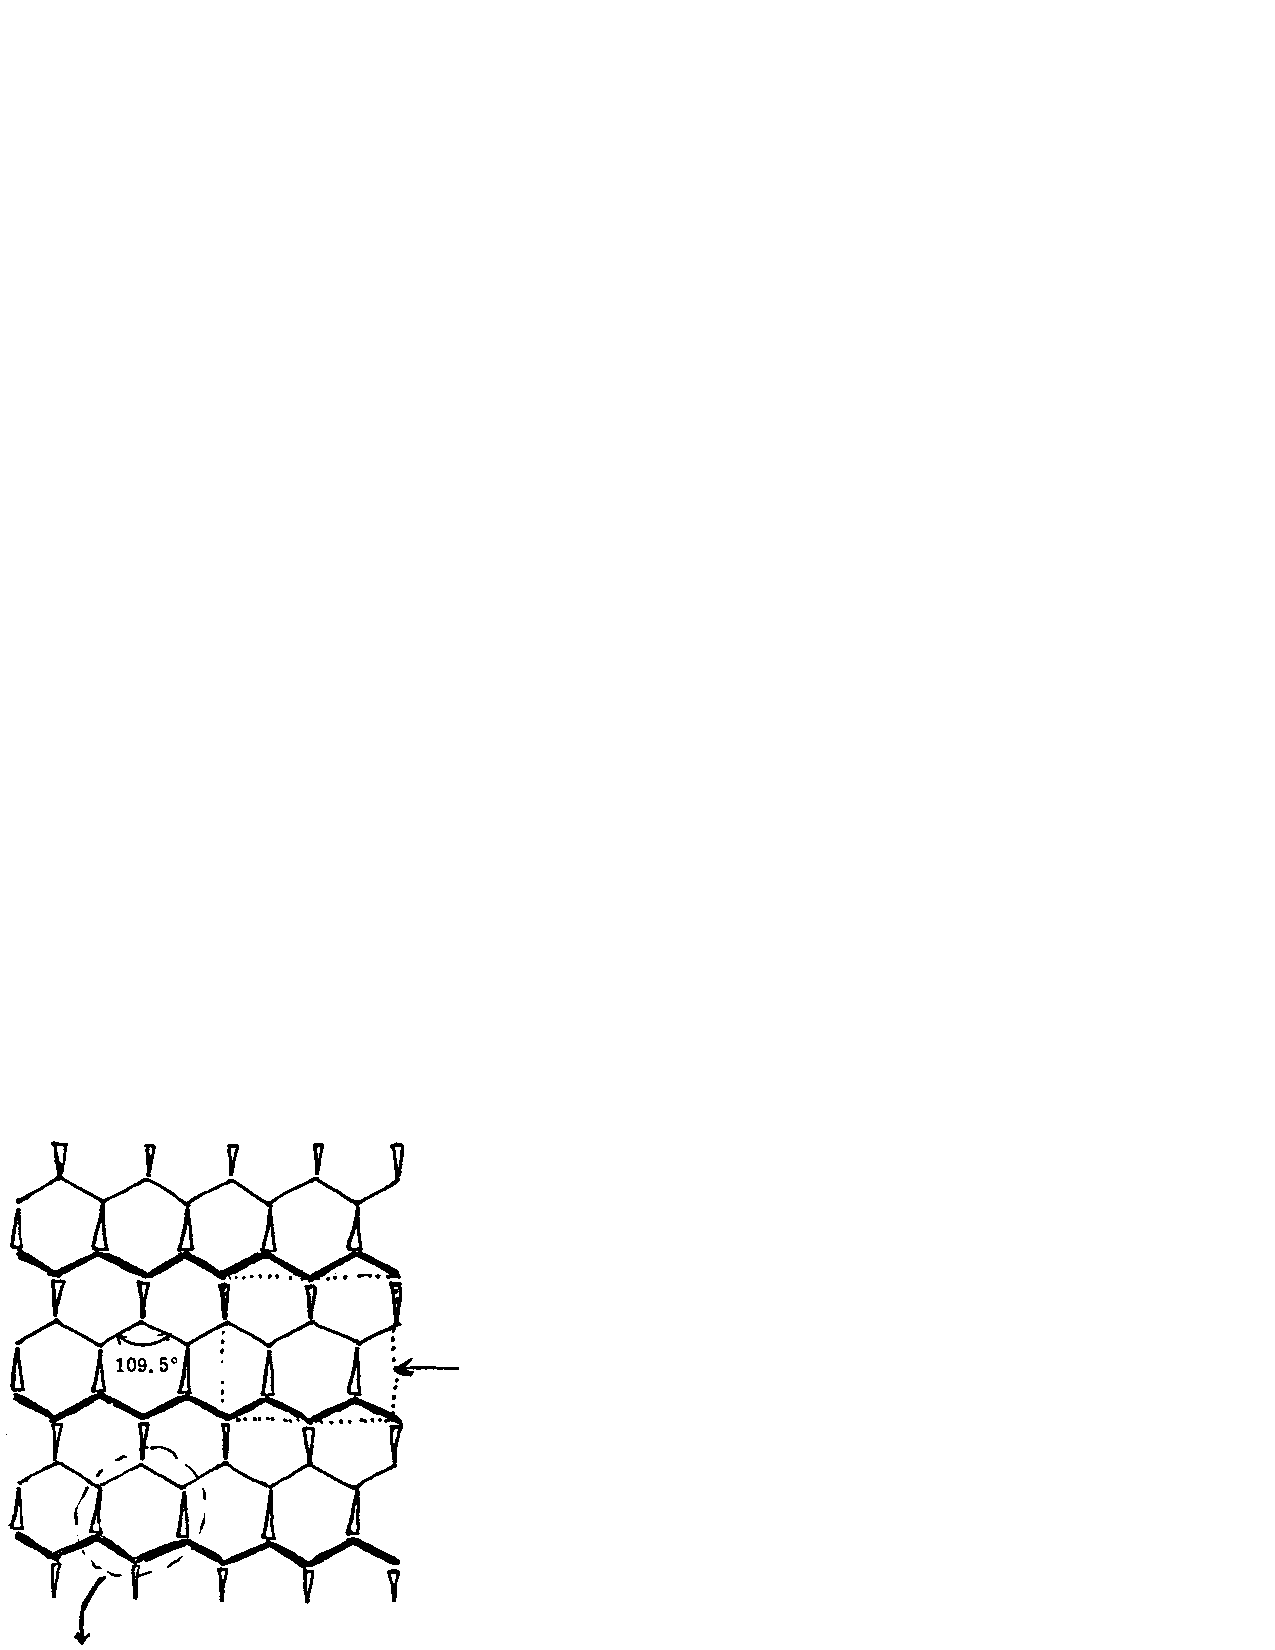
\includegraphics[scale=0.75]{fg8-01}
\end{center}
\caption{The infinite structure constructed using tetrahedral bonding 
plus staggering of bonds on adjacent centers. In this view, we see
chains from left to right with connections between the chains of the
first and second layers.  In addition, each atom of the first layer
has a bond to an atom of the zeroth layer, not shown, and each atom of
the second layer has a bond to the third layer, also not shown. This
structure leads to six-membered rings having the chair configuration,
as shown. The dotted outline here, indicates the region included in
Figure \ref{chap8-fig3}.}
\label{chap8-fig1}
\end{figure}

An alternative view of the infinite structure implicit in Figure
\ref{chap8-fig1}, but not obvious is given in Figure \ref{chap8-fig2}.
In order to aid in comparing Figures \ref{chap8-fig1} and
\ref{chap8-fig2}, we show in Figure \ref{chap8-fig3} the layer numbers
from Figure \ref{chap8-fig1}.


\begin{figure}
\begin{center}
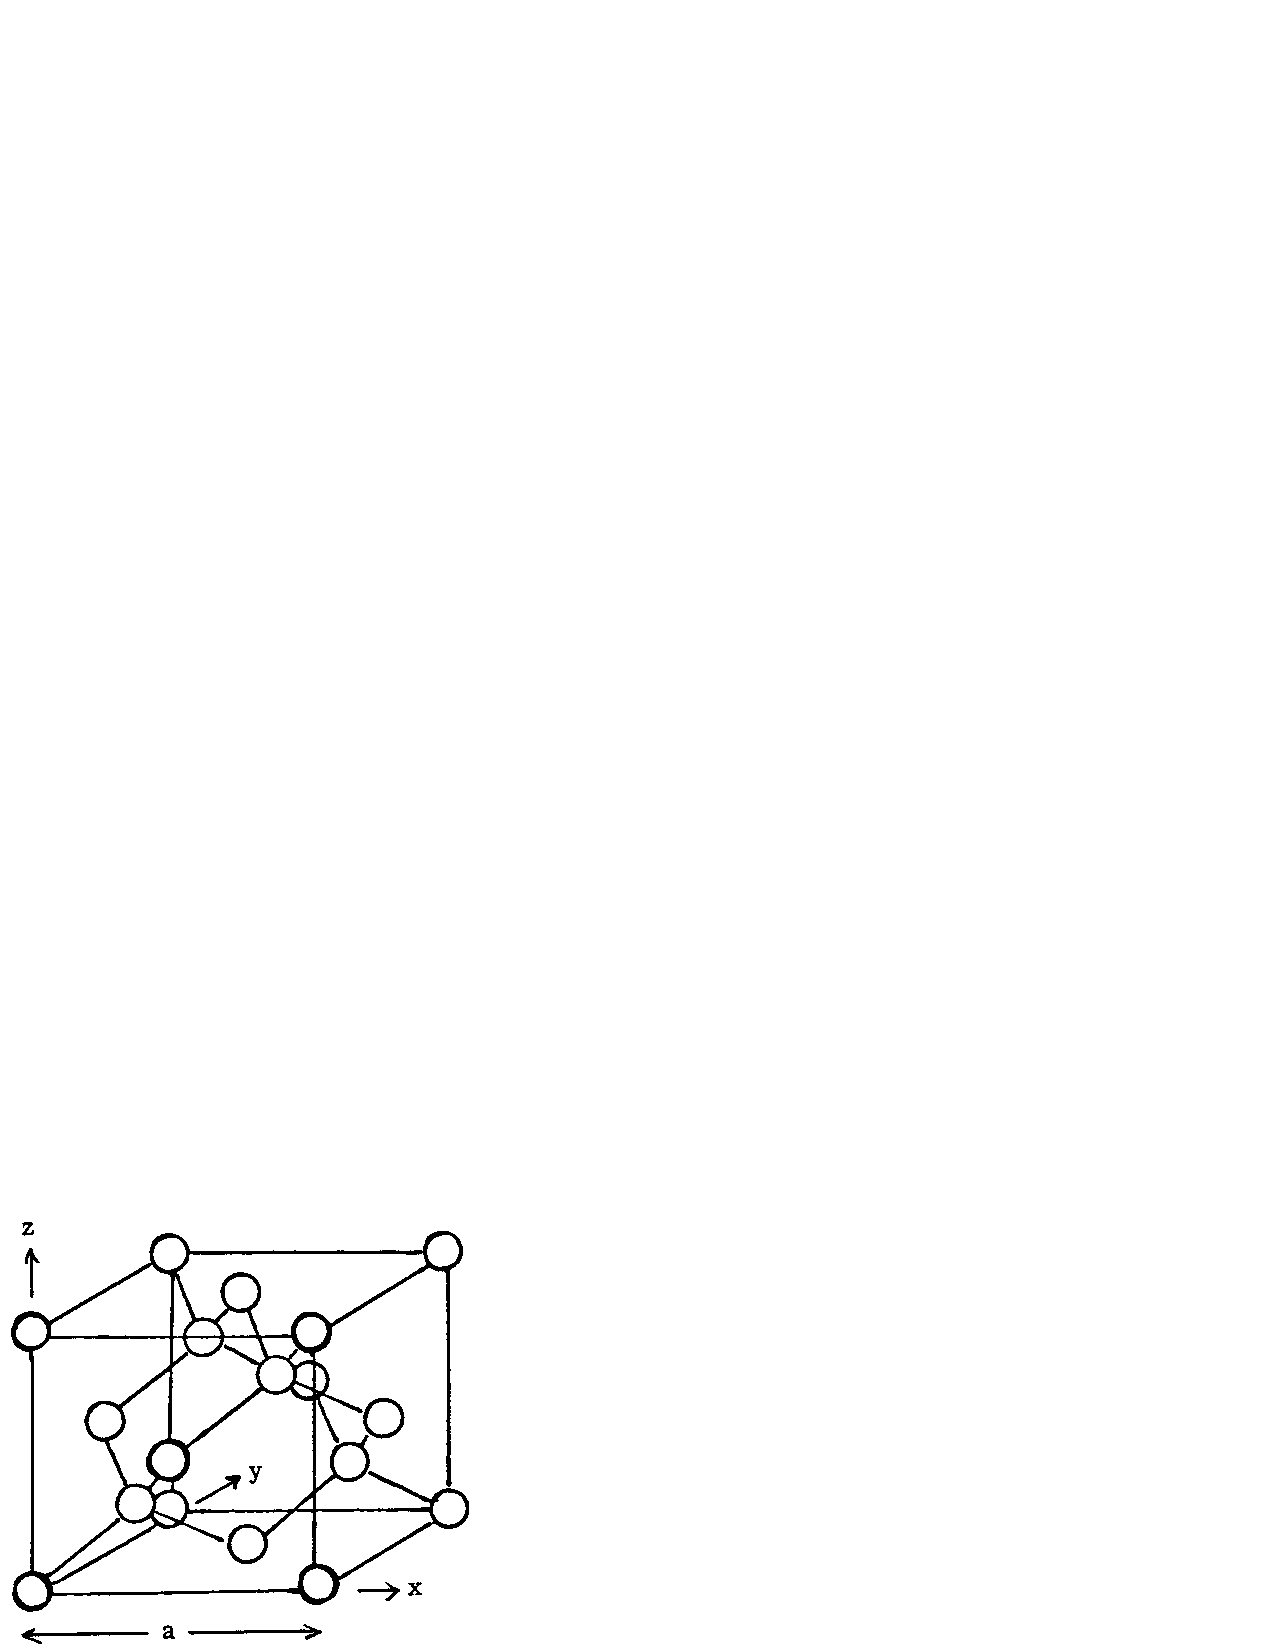
\includegraphics[scale=0.75]{fg8-02}
\end{center}
\caption{The diamond structure (type A4). The structure has atoms at
the corners, (0,0,0), and face centers, (0,${1 \over 2}a$,${1 \over
2}a$), (${1 \over 2}a,0,{1 \over 2}a$), (${1 \over 2}a,{1 \over
2}a,0$), and internally, (${1 \over 4}a,{1 \over 4}a,{1 \over 4}a$),
(${3 \over 4}a,{3 \over 4}a,{1 \over 4}$), (${1 \over 4}a,{3 \over
4}a,{3 \over 4}a$), and (${3 \over 4}a,{1 \over 4}a,{3 \over 4}a$).}
\label{chap8-fig2}
\end{figure}

\begin{figure}
\begin{center}
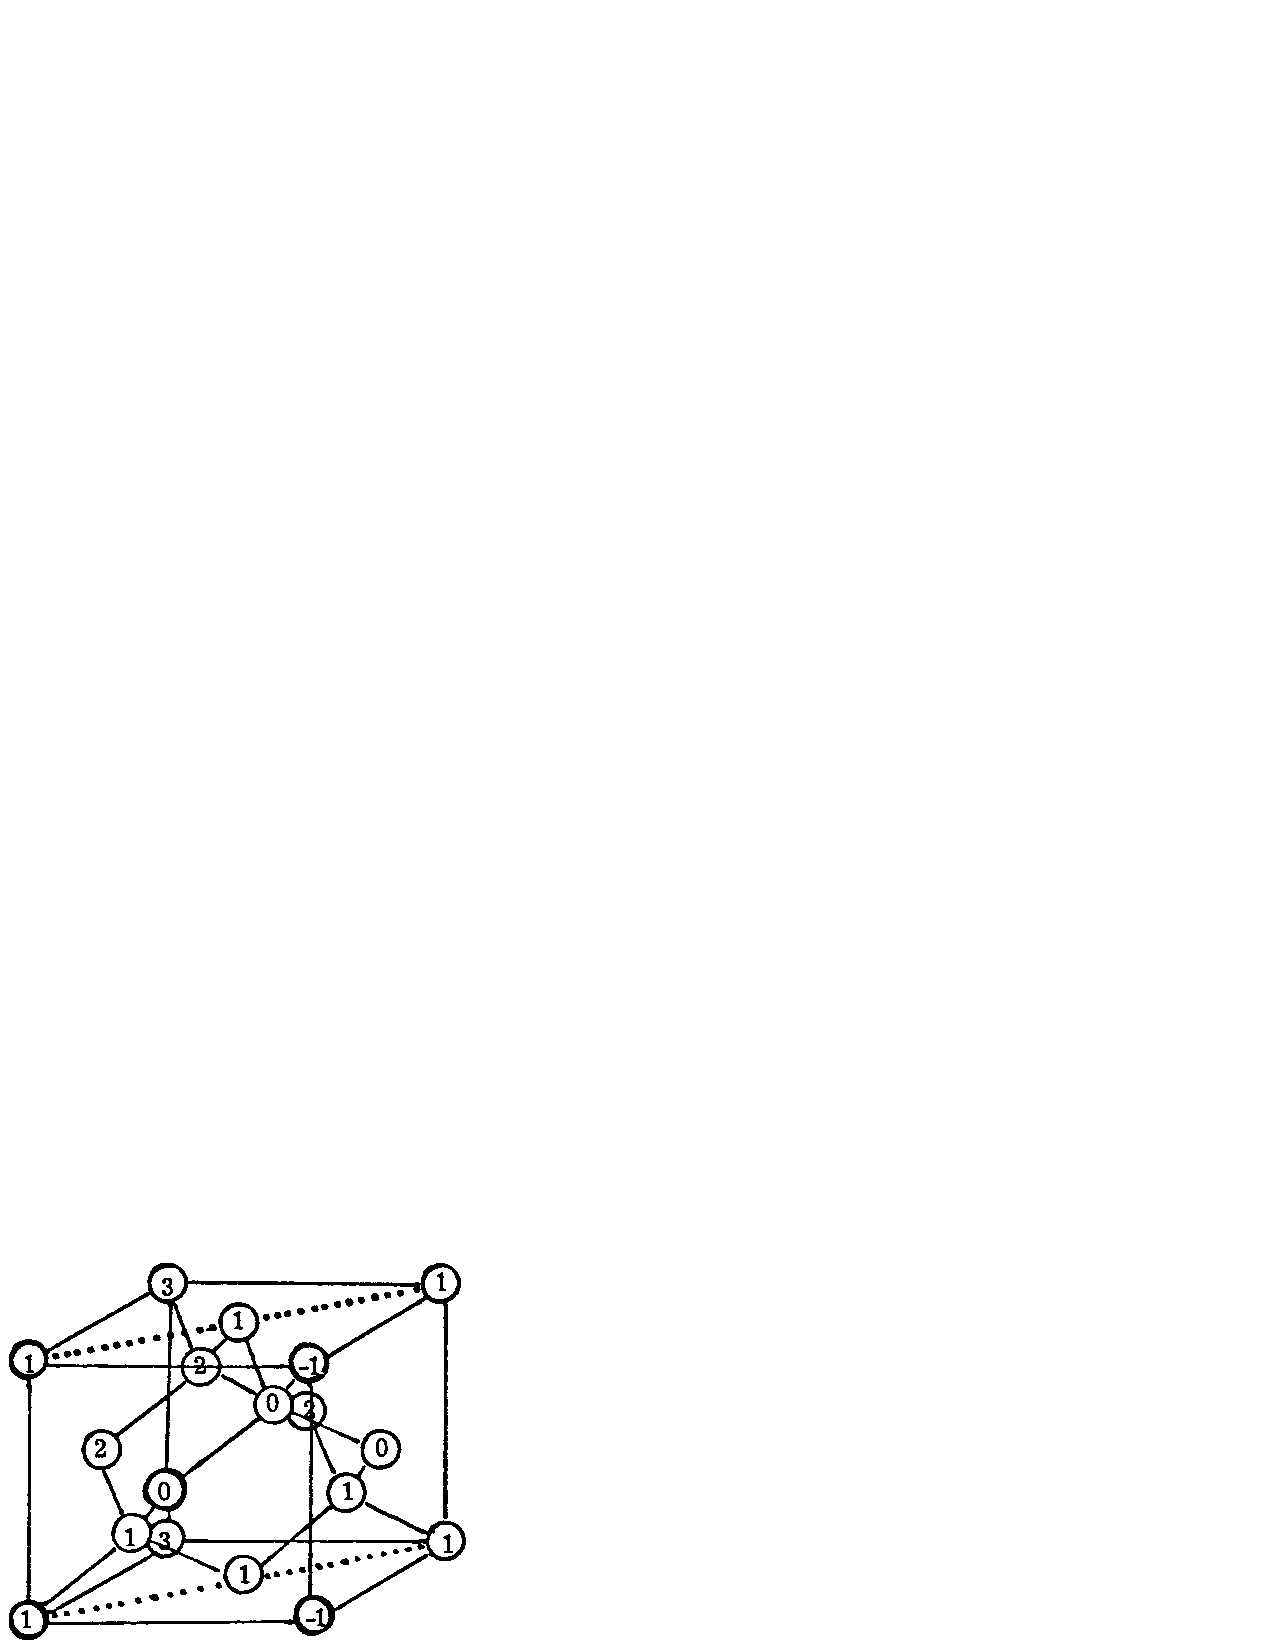
\includegraphics[scale=0.75]{fg8-03}
\end{center}
\caption{The layers from Figure \ref{chap8-fig1} are labelled on the
diamond structure of Figure \ref{chap8-fig2}.  The dotted region of
Figure \ref{chap8-fig3} corresponds to the dotted region in Figure
\ref{chap8-fig1}.}
\label{chap8-fig3}
\end{figure}

The bond distances and bond energies of these crystals are given in Table 
\ref{chap8-tab1}.  Somewhat analogous single bonds should be present in 
H$_3$C$-$CH$_3$, H$_3$Si$-$SiH$_3$, etc.  Indeed, the bond lengths are
comparable, 1.536 \AA\ for H$_3$C$-$CH$_3$ and 1.5445 for diamond, and
2.327 \AA\ for H$_3$Si$-$SiH$_3$ and 2.352 for crystalline Si, as
indicated in Tables \ref{chap8-tab2a}--\ref{chap8-tab2b}.

\begin{table}
\caption{Properties of diamond crystals.}
\label{chap8-tab1}
\begin{tabular}{cccc}\\ \hline

& Bond Distance$^a$ & Cohesive Energy$^b$ & Average Bond\cr
& (\AA) & per atom (kcal) & Energy (0$^{\circ}$K)\cr
& 25$^{\circ}$C & 0$^{\circ}$K\cr

C (diamond) & 1.5445 $\pm$ 0.0001 & 169.4 & 84.70\cr
SiC$^c$ & 1.883$^e$ & 146.31$^d$ & 73.2\cr
Si & 2.3515 $\pm$ 0.0001 & 107.9 & 53.9\cr
Ge & 2.4497 $\pm$ 0.0001 & 88.8 & 44.4\cr
$\alpha$-Sn (gray) & 2.8099 & 72.0 & 36.00\cr
\hline
\end{tabular}\\
$^a$ J. Donohue, The Structure of the Elements, Wiley, New York, 1974.
$^b$ R. Hultgren, P. D. Desai, D. T. Hawkins, M. Gleiser, K. K. 
Kelley, and D. Wagman, Selected Values of the Thermodynamic Properties 
of the Elements, American Society for Metals, Metals Park, Ohio, 1973.
$^c$ Each C as bonded to four Si and each Si to four C. This is 
$\beta$-SiC or cubic SiC. The more stable
form, $\alpha$-SiC, has an hexagonal structure. 
$^d$ NBS Technical Note 270-3. 
$^e$ Wyckoff, {\it loc. cit}.
\end{table}

\begin{table}
\caption{Properties of group IV molecules: Bond lengths (\AA).}
\label{chap8-tab2a}
\begin{tabular}{cccc}\\ \hline
& Single & Bond & Double Bond\cr
& (Crystal) & (H$_3$X$-$XH$_3$) & (X=X)\cr

C & 1.545 & 1.536 & 1.368$^a$\cr
Si & 2.352 & 2.327 & 2.246\cr
Ge & 2.450\cr
Sn & 2.810\cr
\hline
\end{tabular}
\end{table}

\begin{table}
\caption{Properties of group IV molecules: Bond energy (kcal at
0$^{\circ}$K).} 
\label{chap8-tab2b}
\begin{tabular}{cccc}\\ \hline
\multicolumn{2}{c}{Single Bond}& Double Bond & Diatomic\cr
(Cyrstal) & (H$_3$X$-$SH$_3$) & (X=X)\cr

84.70 & 89.9 & 124.8$^a$ & 40.1\cr
53.9 & 74. & 74.0 & 20.1\cr
44.4 & & 65.0 & 20.6\cr
36.0 & & 45.9 & 9.9\cr
\hline
\end{tabular}\\
$^a$ Here we use the properties of the ${^3\Sigma}^-_g$ state of 
C$_2$ in order to compare with other species.
\end{table}

A discussion of bond energies is somewhat trickier. We can calculate
an average bond energy in the crystal by comparing the total energy
per atom in the crystal with the energy of a free atom.  This
difference is called the {\it cohesive energy}, e.g., 169.4 kcal for
diamond. In order to relate this to an average bond energy, we note
first that there are four bonds broken to each atom.  Thus, for $N =
10^{22}$ atoms, we might think that $4N$ bonds were broken.  However,
this leads to counting each broken bond twice so that the net number
of bonds broken is $2N$. Thus, from Table \ref{chap8-tab1}, we obtain
average bond energies of ${\bar{D}} =$ 84.7 kcal for diamond, and
${\bar{D}} =$ 53.9 kcal for Si crystal, which can be compared with the
values of $D_0 = 89.9$ kcal for H$_3$C$-$CH$_3$ and $D+0 = 74$ kcal
for H$_3$Si$-$SiH$_3$.  The comparison is pretty good for C, but
terrible for Si. The major problem here is that even when a molecule
is tetrahedral, e.g., CH$_4$ or SiH$_4$, the energy to break the first
bond may be very different from that required to break successive
bonds. Thus, from Chapter 6 we have the results in Table
\ref{chap8-tab3}.  Here we see that the difference between the first
bond energy and the average, $D_1 - {\bar{D}}$ in Table
\ref{chap8-tab3}, is 5.5 for C and 15.6 for Si, explaining most of the
discrepancy.  Some thermodynamic properties of group IV solids are
summarized in Table \ref{chap8-tab4}.

\begin{table}
\caption{Comparisons of bond energies (kcal, 300$^{\circ}$K).}
\label{chap8-tab3}
\begin{tabular}{ccc}\\ \hline

& C & Si\cr

$D_1 (XH_4 \rightarrow XH_3 + H)$ & 104.8 & 91.6\cr
$D_2 (XH_3 \rightarrow XH_2 + H)$ & 109.4 & 69.7\cr
$D_3 (XH_2 \rightarrow XH + H)$ & 102.0 & 74.2\cr
$D_4 (XH \rightarrow X + H)$ & 81.0 & 68.5\cr
${\bar{D}}$, average bond energy & 99.3 & 76.0\cr
${\bar{D}} - {\bar{D}}$ & 5.5 & 15.6\cr
\hline
\end{tabular}
\end{table}

\begin{table}
\caption{Thermodynamic properties of group IV solids.}
\label{chap8-tab4}
\begin{tabular}{cccccc}\\ \hline

& $T_{mp}$ & $\Delta H_{fusion}$ & $T_{bp}$ &\multicolumn{2}{c}{$\Delta 
H_v$}\cr
& & & & $0^{\circ}$ & 298$^{\circ}$K\cr
& ($^{\circ}$K) & (kcal) & ($^{\circ}$K) &\multicolumn{2}{c}{(kcal)}\cr

C (graphite)$^b$ & (4100)$^c$ & -- & 4100$^c$ & 170.0 & 171.3 $\pm$ 
1.0\cr
Si & 1685 & 12.08 & 3540 & 107.9 & 108. 9 $\pm$ 1.0\cr
Ge & 1210.4 & 8.83 & 3107 & 88.8 & 89. 5 $\pm$ 0.5\cr
Sn$^a$ & 505.06 & 1.68 & 2876 & 72.0 & 72.0 $\pm$ 0.4\cr
Pb & 600.6 & 1.147 & 2023 & 46.8 & 46.6 $\pm$ 0.3\cr
\hline
\end{tabular}\\
$^a$ $T_{\alpha \beta} = 2.862^{\circ}$K, $\Delta H_{\alpha 
\beta} = 0.47$ kcal.
$^b$ $T 298.15^{\circ}$, $\Delta H = 0.453$ kcal for conversion of 
graphite to diamond.  At $T = O^{\circ}$K, $\Delta H = 0.580$ kcal.
$^c$ At atmospheric pressure, graphite sublimes without 
melting.  This value is extrapolated.
\end{table}

\subsection{The Sphalerite or Zincblende Structure}

Replacing each Ge atom of the diamond structure, alternatively with Ga and 
As so that each Ga is bonded to four As, and each As to four Ga, leads to 
the sphalerite structure shown in Figure \ref{chap8-fig4}.

\begin{figure}
\begin{center}
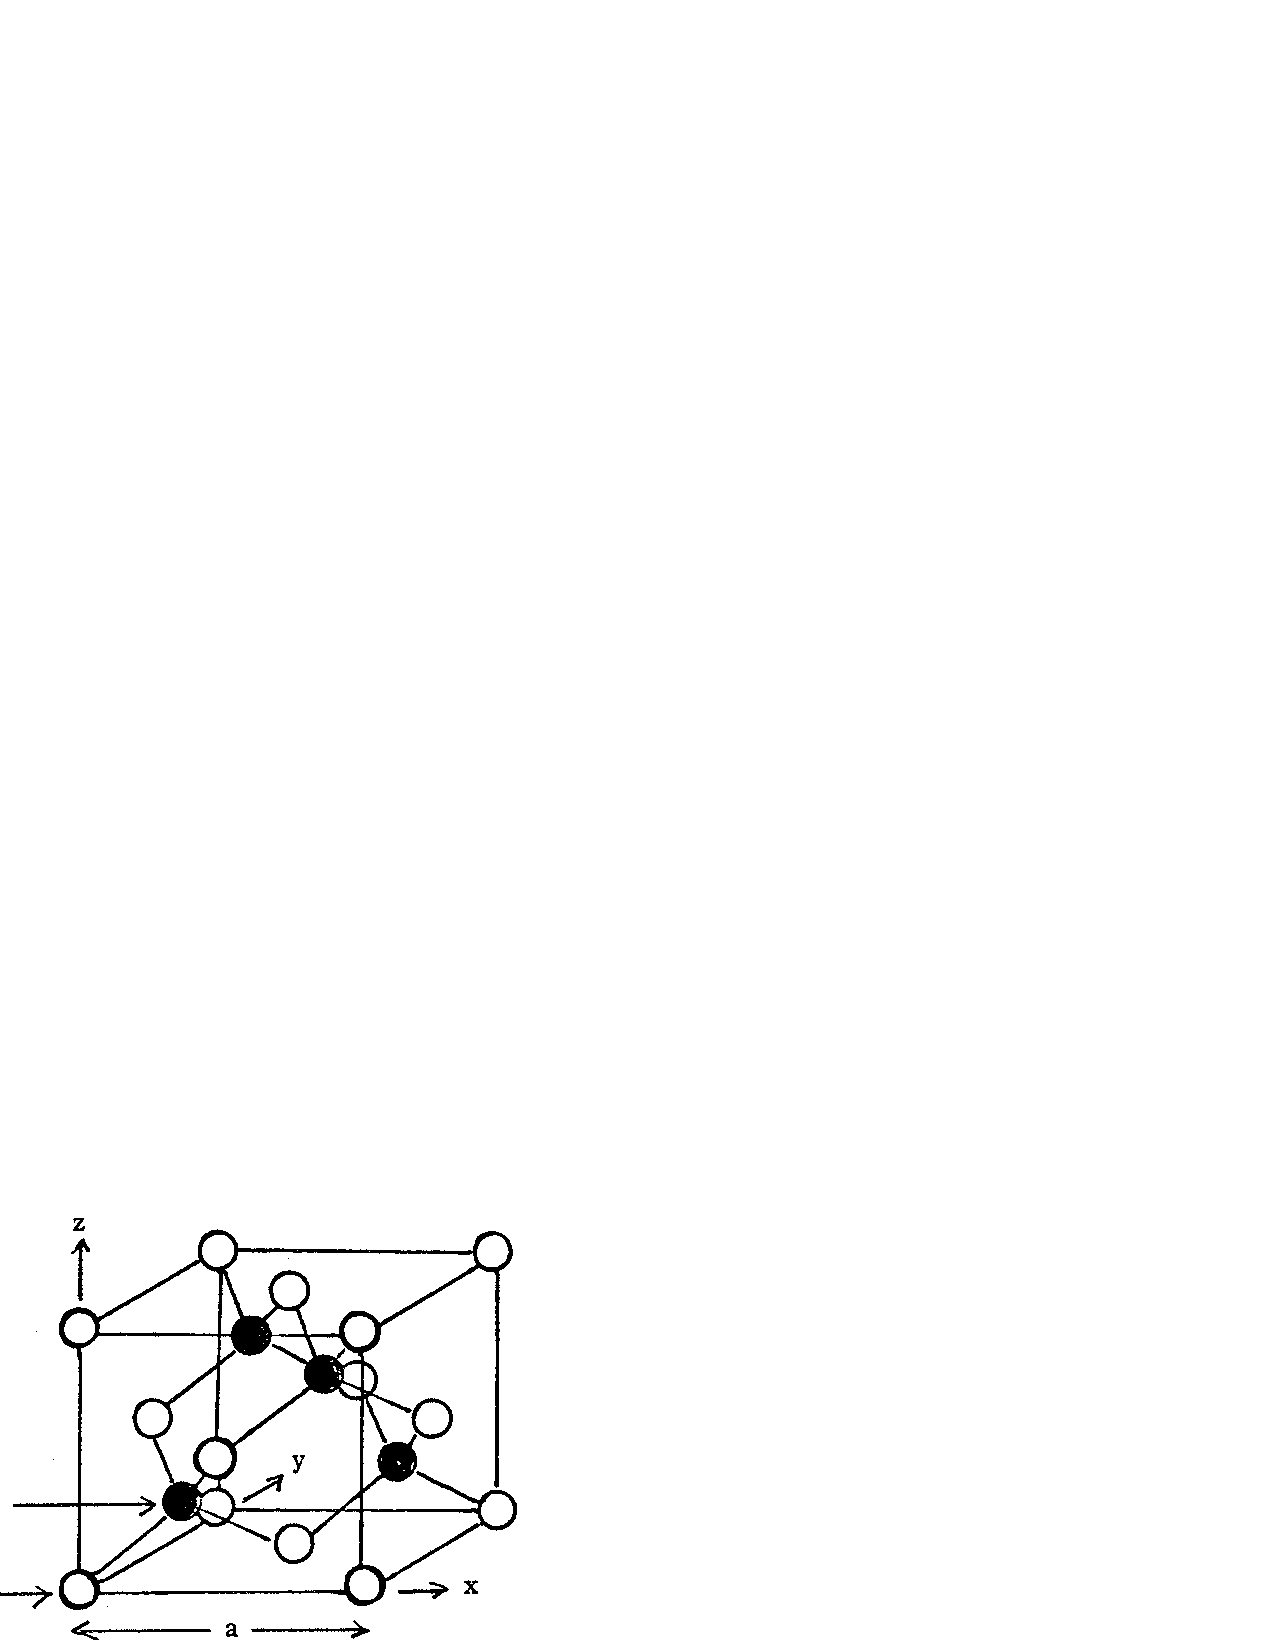
\includegraphics[scale=0.75]{fg8-04}
\end{center}
\caption{The sphalerite or GaAs structure. This
is identical to diamond except that two types of atoms are
present. Each Ga is in a tetrahedron of As, and each As has four Ga
nearest neighbors. If $a$ is the size of the cubic unit cell, there
are Ga at (${1 \over 4}a$,${1 \over 4}a$,${1 \over 4}a$),(${3 \over
4}a$,${3 \over 4}a$,${1 \over 4}a$),(${1 \over 4}a$,${3 \over 4}a$,${3
\over 4}a$), and (${3 \over 4}a$,${1 \over 4}a$,${3 \over 4}a$) and,
As at the corners (0,0,0), and face centers (0,${1 \over 2}a$,${1
\over 2}a$),(${1 \over 2}a$, 0,${1 \over 2}a$), and (${1 \over
2}a$,${1 \over 2}a$,0).} 
\label{chap8-fig4}
\end{figure}


Making covalent bonds to each atom, we might have expected just three
covalent bonds to each Ga, since there are three valence electrons,
and just three covalent bonds to each As plus a lone pair.  Indeed,
one can visualize the bonding in GaAs in this way, as indicated in
Figure \ref{chap8-fig5}, where the three covalent bonds to each Ga and
As are shown normally, and the fourth bond is indicated as an As 4s
lone pair that is coordinated to an empty orbital on the Ga, a
donor-acceptor or Lewis basis-Lewis acid bond.  The four bonds to each
atom would adjust so as to be equivalent, but one can think of each
bond as having 3/4 covalent character plus 1/4 donoracceptor
character.

\begin{figure}
\begin{center}
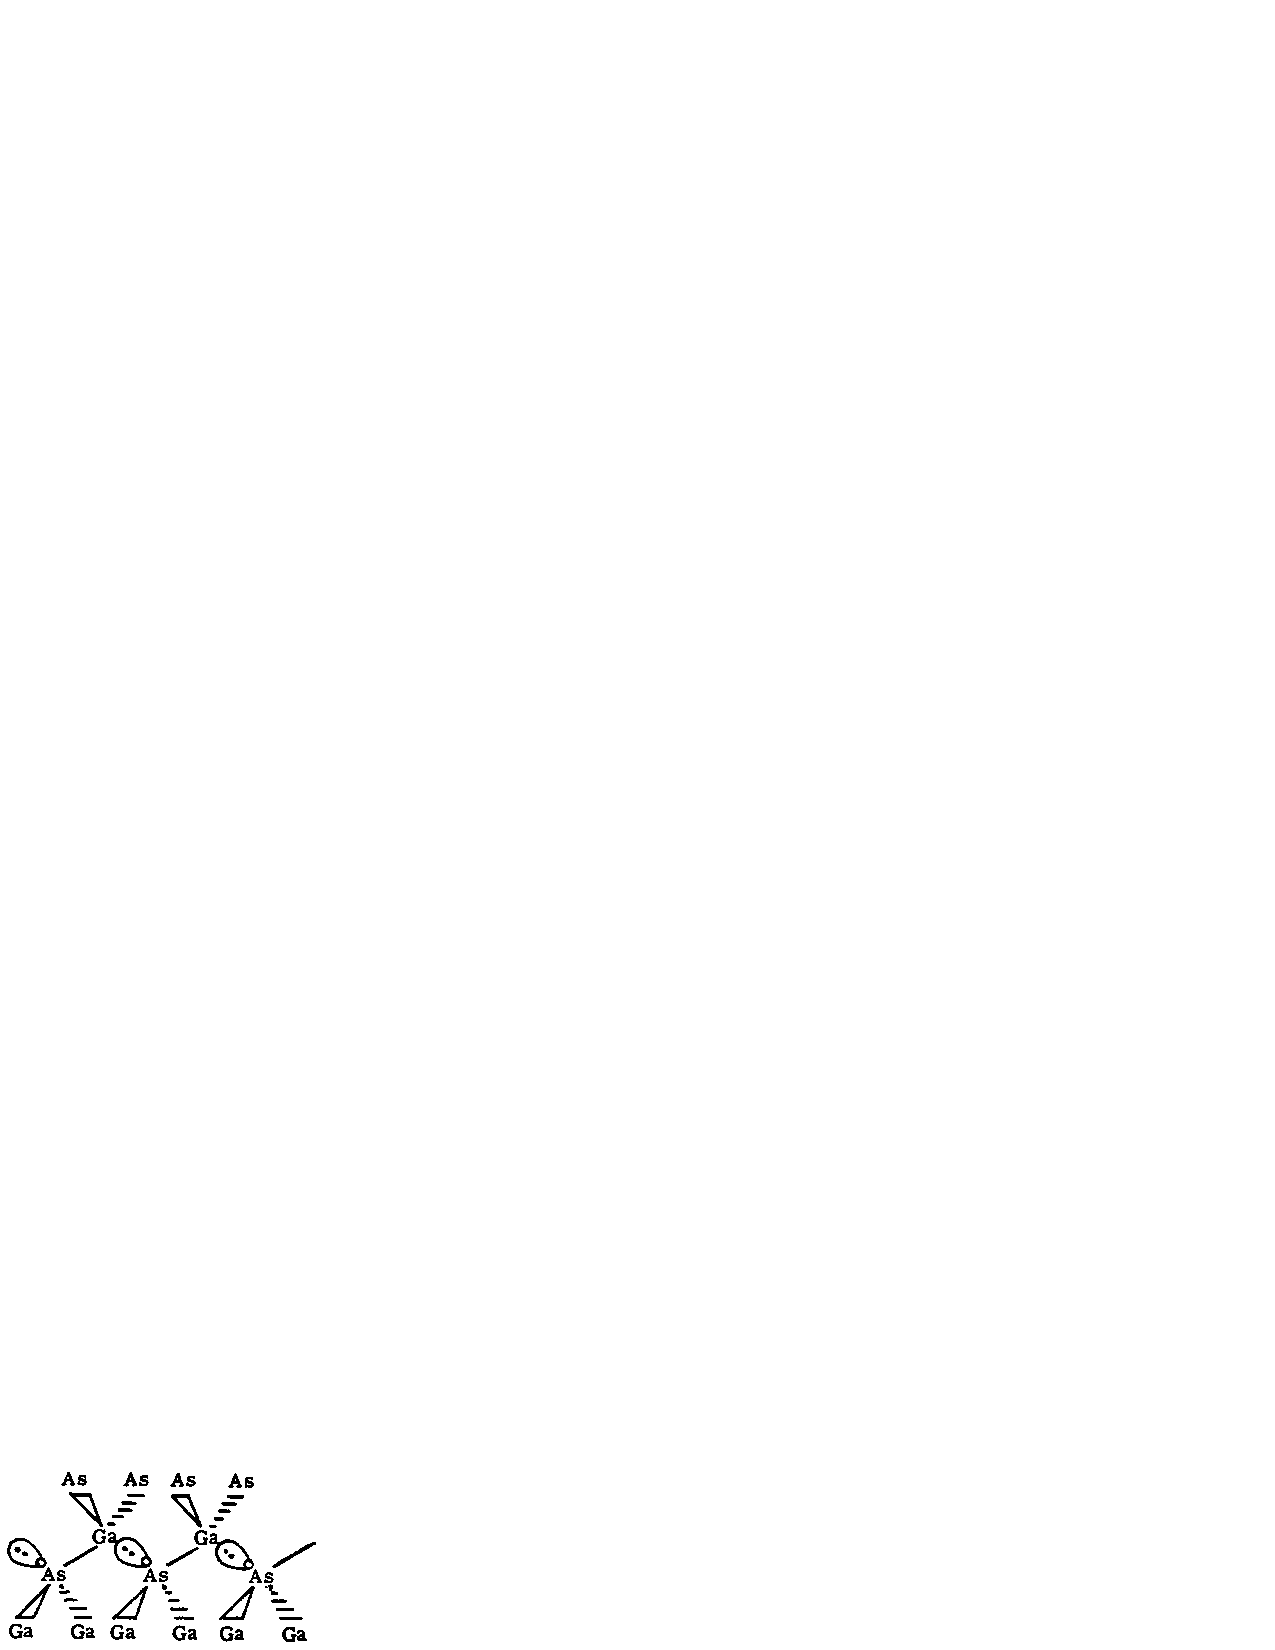
\includegraphics[scale=0.75]{fg8-05}
\end{center}
\caption{}
\label{chap8-fig5}
\end{figure}


Analogous compounds XY can be formed from most combinations of X = B,
Al, Ga, and In, and Y = N, P, As, and Sb; called III-V compounds, from
the columns of the periodic table. Except for the cases with Y = N,
all lead to the cubic crystal shown in Figure \ref{chap8-fig4}.  As
shown in Tables
\ref{chap8-tab5} and \ref{chap8-tab6}, the bond distances are III-V
and group IV compounds of the same row lead to nearly identical bond
distances, within 0.005 to 0.02 \AA); however, the bond energy of the
III-V is always about 10 \% weaker. The latter trend is probably
due to the partial donor-acceptor character of the bond.

\begin{table}
\caption{Average bond distance$^a$ and average bond 
energy$^b$ for the III-V compounds, cubic form.}
\label{chap8-tab5}
\begin{tabular}{ccccc}\\ \hline

& N & P & As & Sb\cr

B & 1.565\AA & 1.965\AA & 2.069\AA\cr
& 77.1 kcal$^c$ & 57.2 kcal\cr
Al & & 2.360\AA & 2.43$^{{\underline{4}}}$\AA & 2.656\AA\cr
& 66.8 kcal$^c$ & 48.3 kcal & 44.5 kcal\cr
Ga & & 2.360\AA & 2.448\AA & 2.640\AA\cr
& 51.4 kcal$^c$ & 40.6 kcal & 38.9 kcal & 34.7 kcal\cr
In & & 2.541 \AA & 2.614 \AA & 2.805\AA\cr
& 64.0 kcal$^c$ & 38.6 kcal & 36.1 kcal & 32. 0 kcal\cr
\hline
\end{tabular}\\
$^a$ Wyckoff, {\it loc. cit}. 
$^b$ NBS Technical Note 270-3. 
$^c$ Based on the cohesive energy for a different structure.
\end{table}

\begin{table}
\caption{Comparison of properties of the M-V and group IV compounds
from the same row of the periodic table.}
\label{chap8-tab6}
\begin{tabular}{ccccc}\\ \hline
&\multicolumn{2}{c}{R}&\multicolumn{2}{c}{\={D}}\cr
&\multicolumn{2}{c}{(\AA)} &\multicolumn{2}{c}{(kcal)}\cr

C$_{\rm diamond}$/BN & 1.545 & 1.565 & 84.7 & 77.1\cr
Si/AlP & 2.352 & 2.360 & 53.9 & 48.3\cr
Ge/GaAs & 2.450 & 2.448 & 44.4 & 38.9\cr
$\alpha$-Sn/InSb & 2.810 & 2.805 & 36.0 & 32.0\cr
\hline
\end{tabular}
\end{table}

\section{Semiconducting Properties}

\subsection{Intrinsic Semiconductors}

In the diamond structure, each of the four electrons of each atom is
involved in a covalent bond to each of its four neighbors. In order to
conduct electricity, we must excite an electron out of one of these
bonds into the bond of a distant atom, as in Figure \ref{chap8-fig6}.


\begin{figure}
\begin{center}
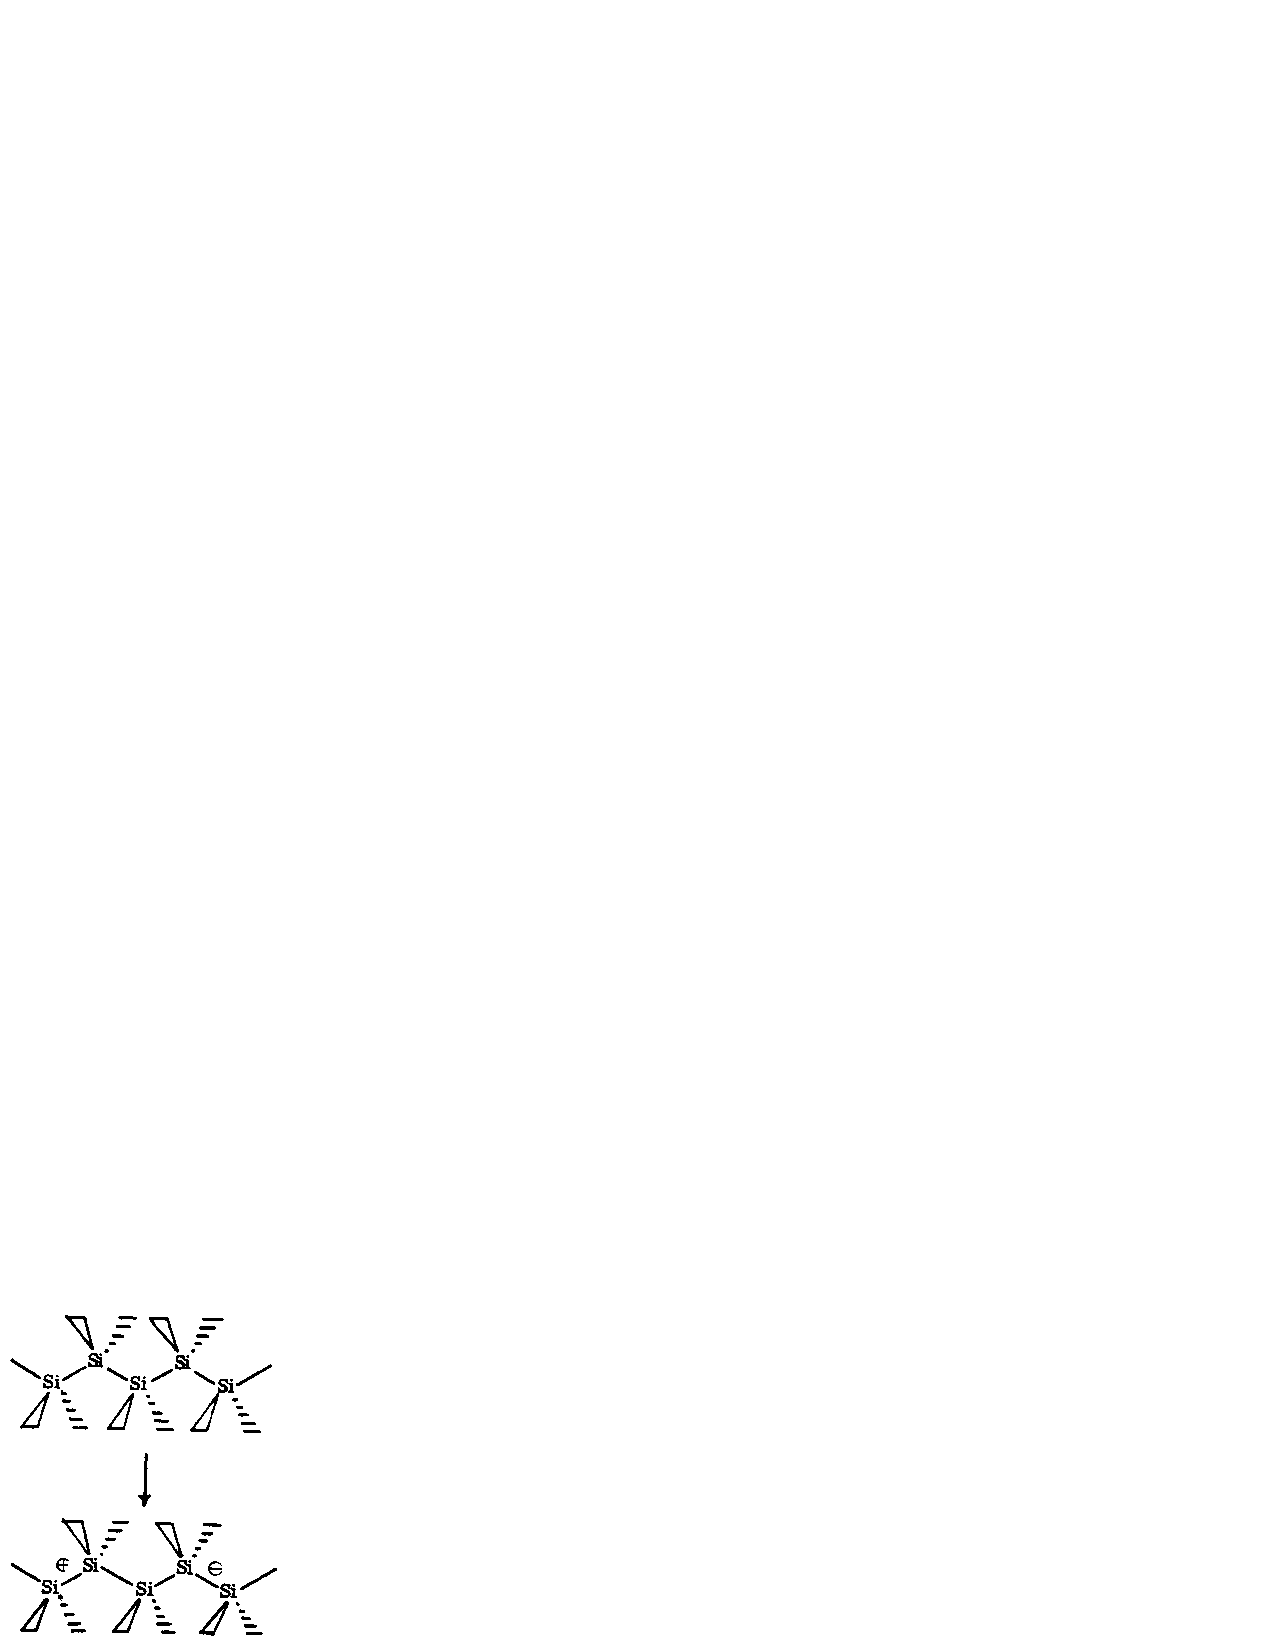
\includegraphics[scale=0.75]{fg8-06}
\end{center}
\caption{}
\label{chap8-fig6}
\end{figure}

To do this costs a finite amount of energy, 1.1 eV for Si, so that a
perfect crystal of Si would be an insulator at room temperature.  Such
conduction properties are usually discussed in terms of the occupied
and empty molecular orbitals of the system. Because there is a nearly
infinite number, 10$^{22}$/cc, of atoms, the energies of the occupied
molecular orbitals form a continuum of levels, called the {\it valence
band}, as do the energies of the empty orbitals, called the {\it
conduction band}.  However, there is a finite energy gap separating
the highest molecular orbital, HOMO, or valence band maximum, VBM,
from the lowest unoccupied molecular orbital, LUMO, or conduction band
minimum, CBM.  This energy diagram is sketched in Figure
\ref{chap8-fig7} and some of the energy quantities for Si are defined
in Figure \ref{chap8-fig8}.

\begin{figure}
\begin{center}
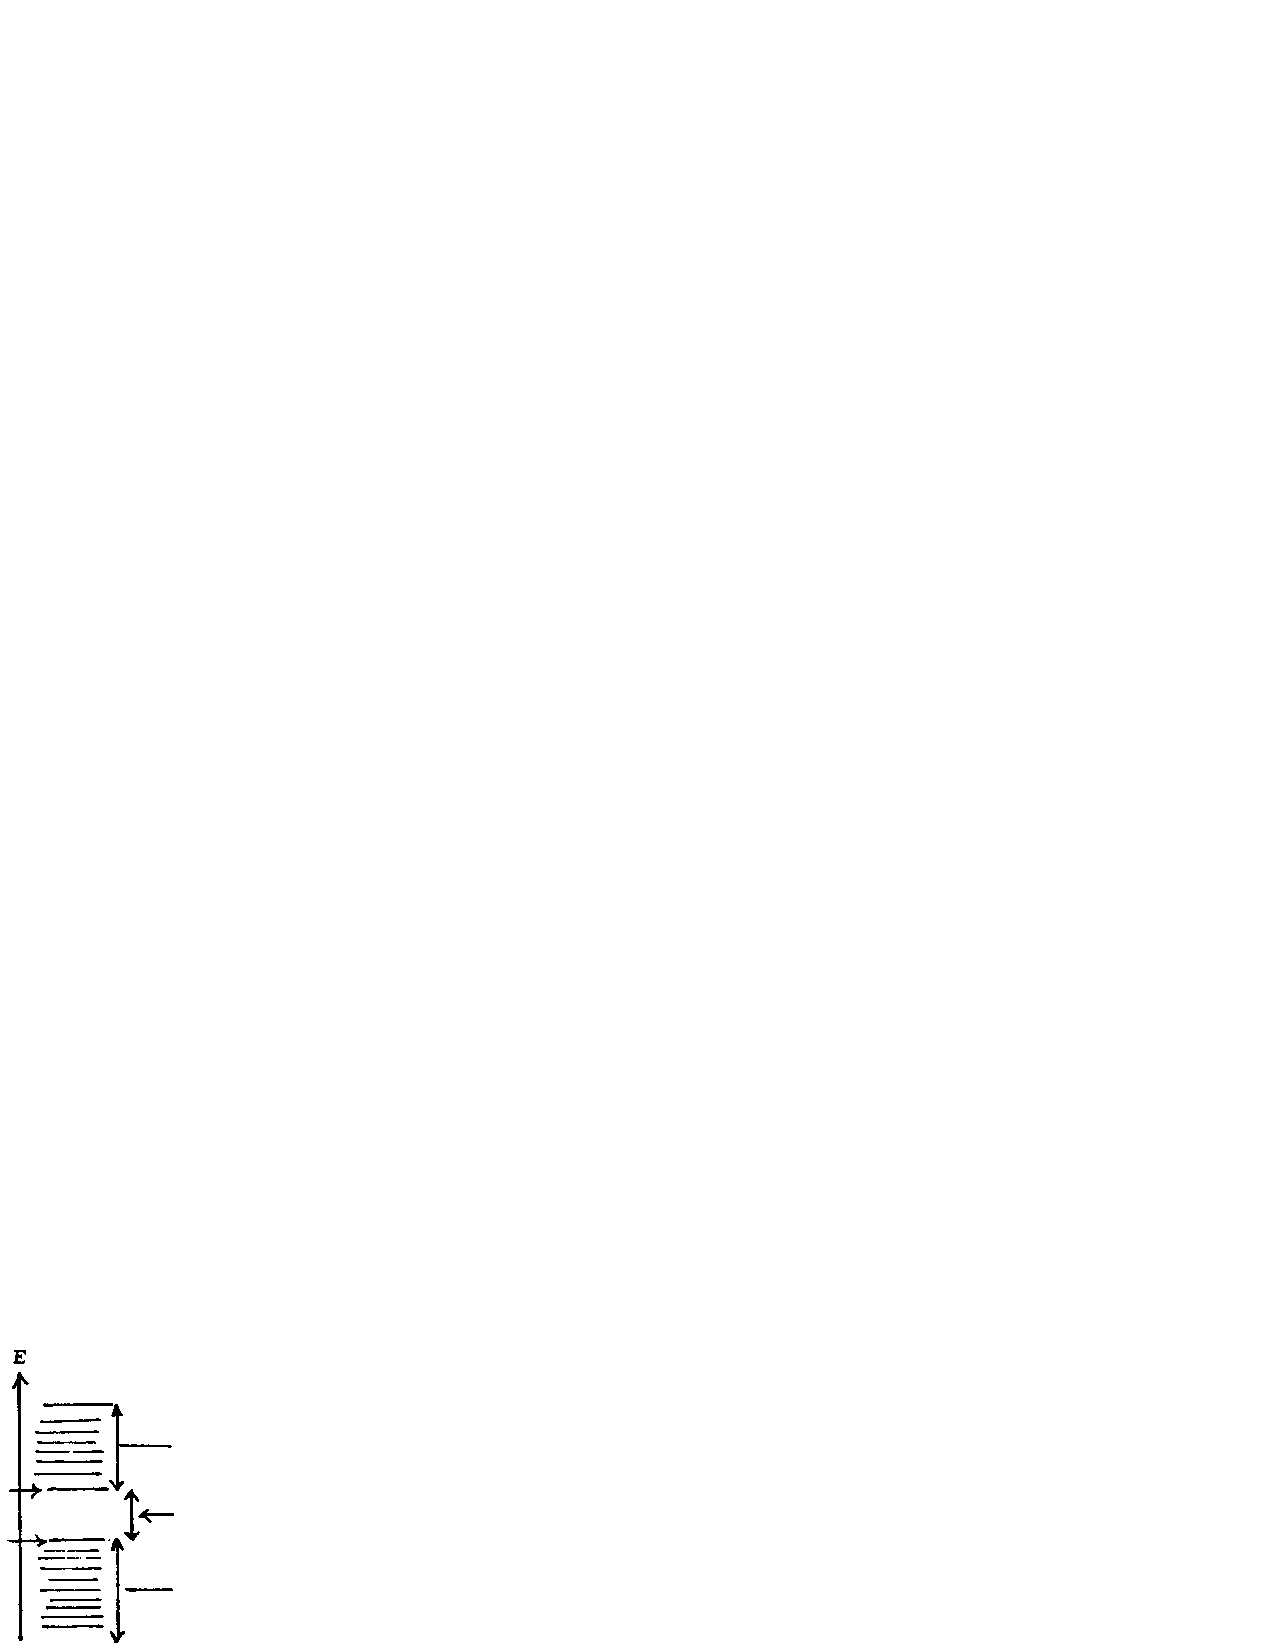
\includegraphics[scale=0.75]{fg8-07}
\end{center}
\caption{Conducting (top) and valence (bottom) bands for an intrinsic semiconductor.}
\label{chap8-fig7}
\end{figure}

\begin{figure}
\begin{center}
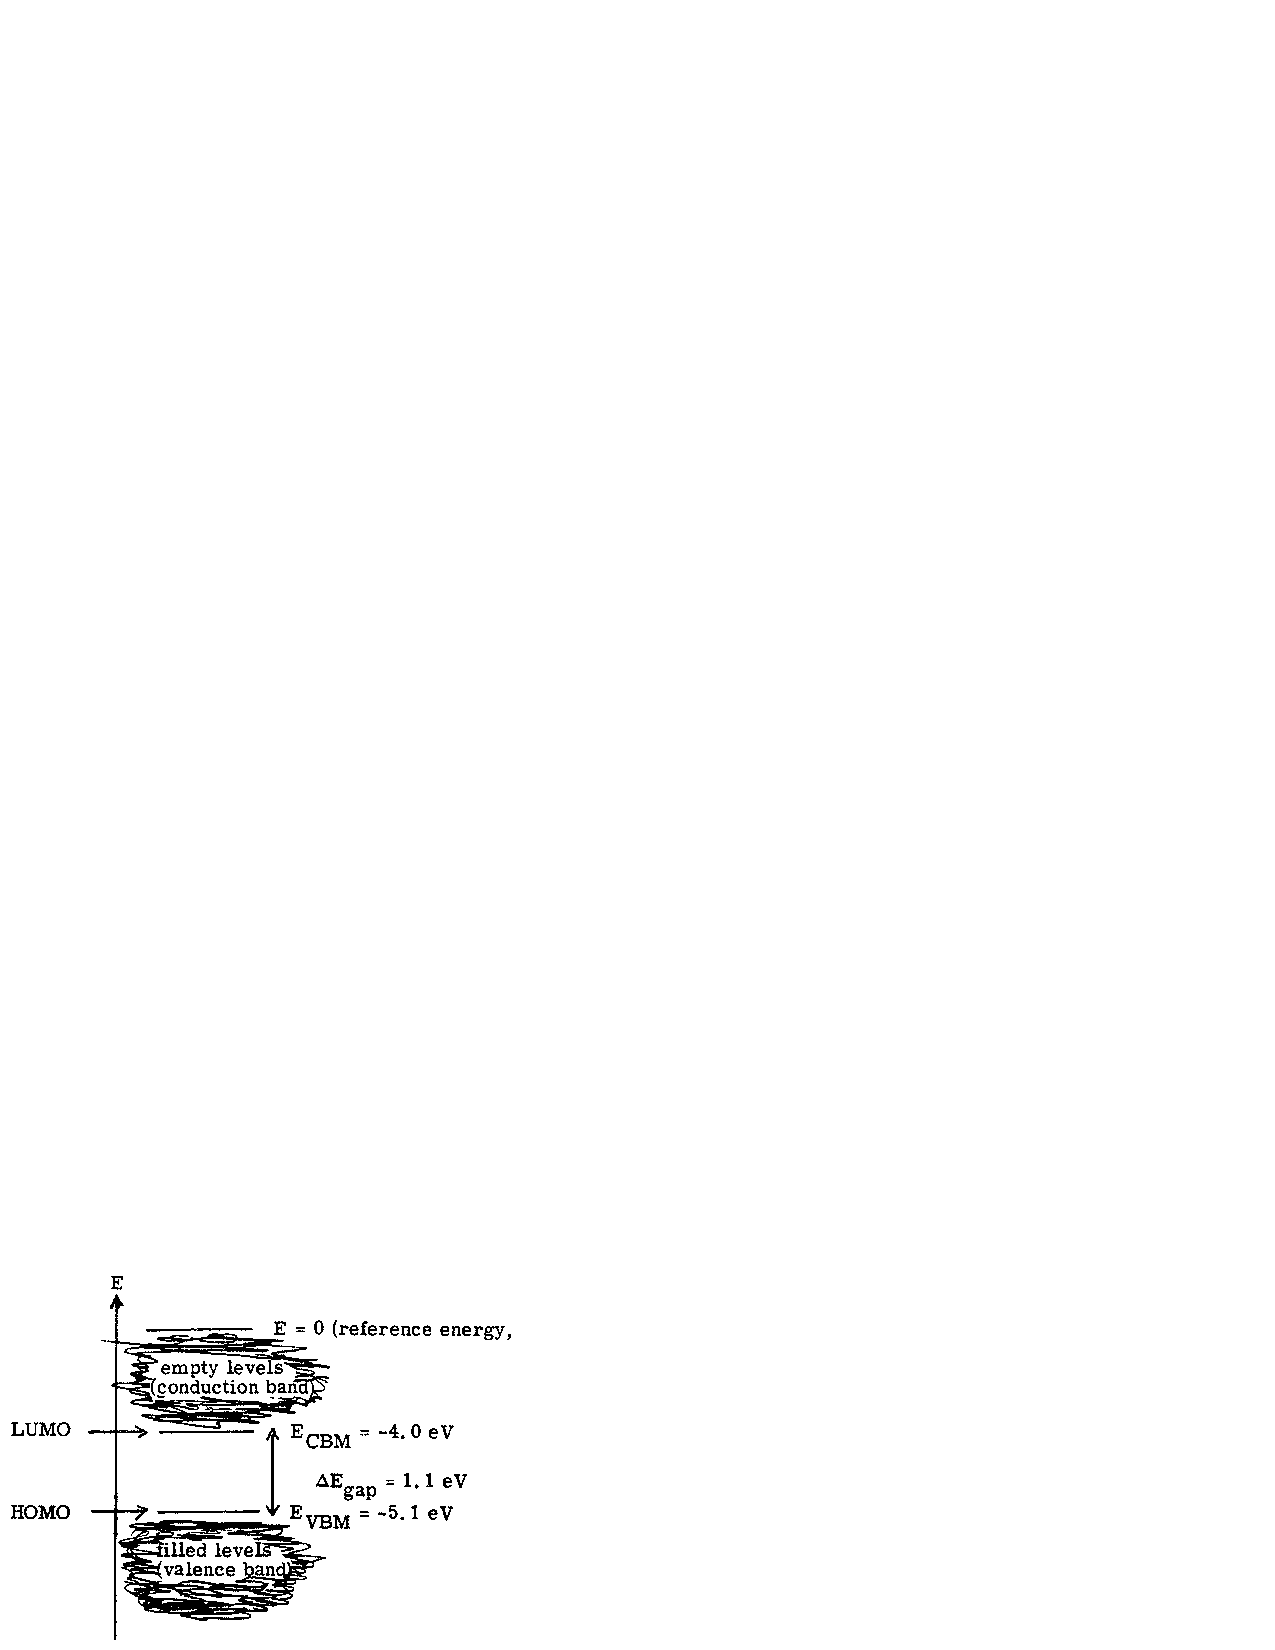
\includegraphics[scale=0.75]{fg8-08}
\end{center}
\caption{The energy levels for Si.}
\label{chap8-fig8}
\end{figure}


At 0$^{\circ}$K, all the electrons are in the valence band, no
electrons are in the conduction band, and the material will not
conduct electricity.  At finite temperature, some of the electrons are
excited from the valence band to the conduction band; however, at room
temperature, this fraction is proportional to
\begin{equation}
e^{-{E_{gap} \over 2kT}} = e^{-{1.1 \over 0.05}} = 2.8 \times 10^{-10},
\end{equation}
still a quite small value.

There are two ways that Si can be made conducting.  One is to put extra 
electrons in the conduction band.  Since there is a continuum of nearby 
orbitals, application of an electron field, say a battery, will cause 
the electron to more toward the positive pole of the battery, as
indicated in Figure \ref{chap8-fig9}(b).

\begin{figure}
\begin{center}
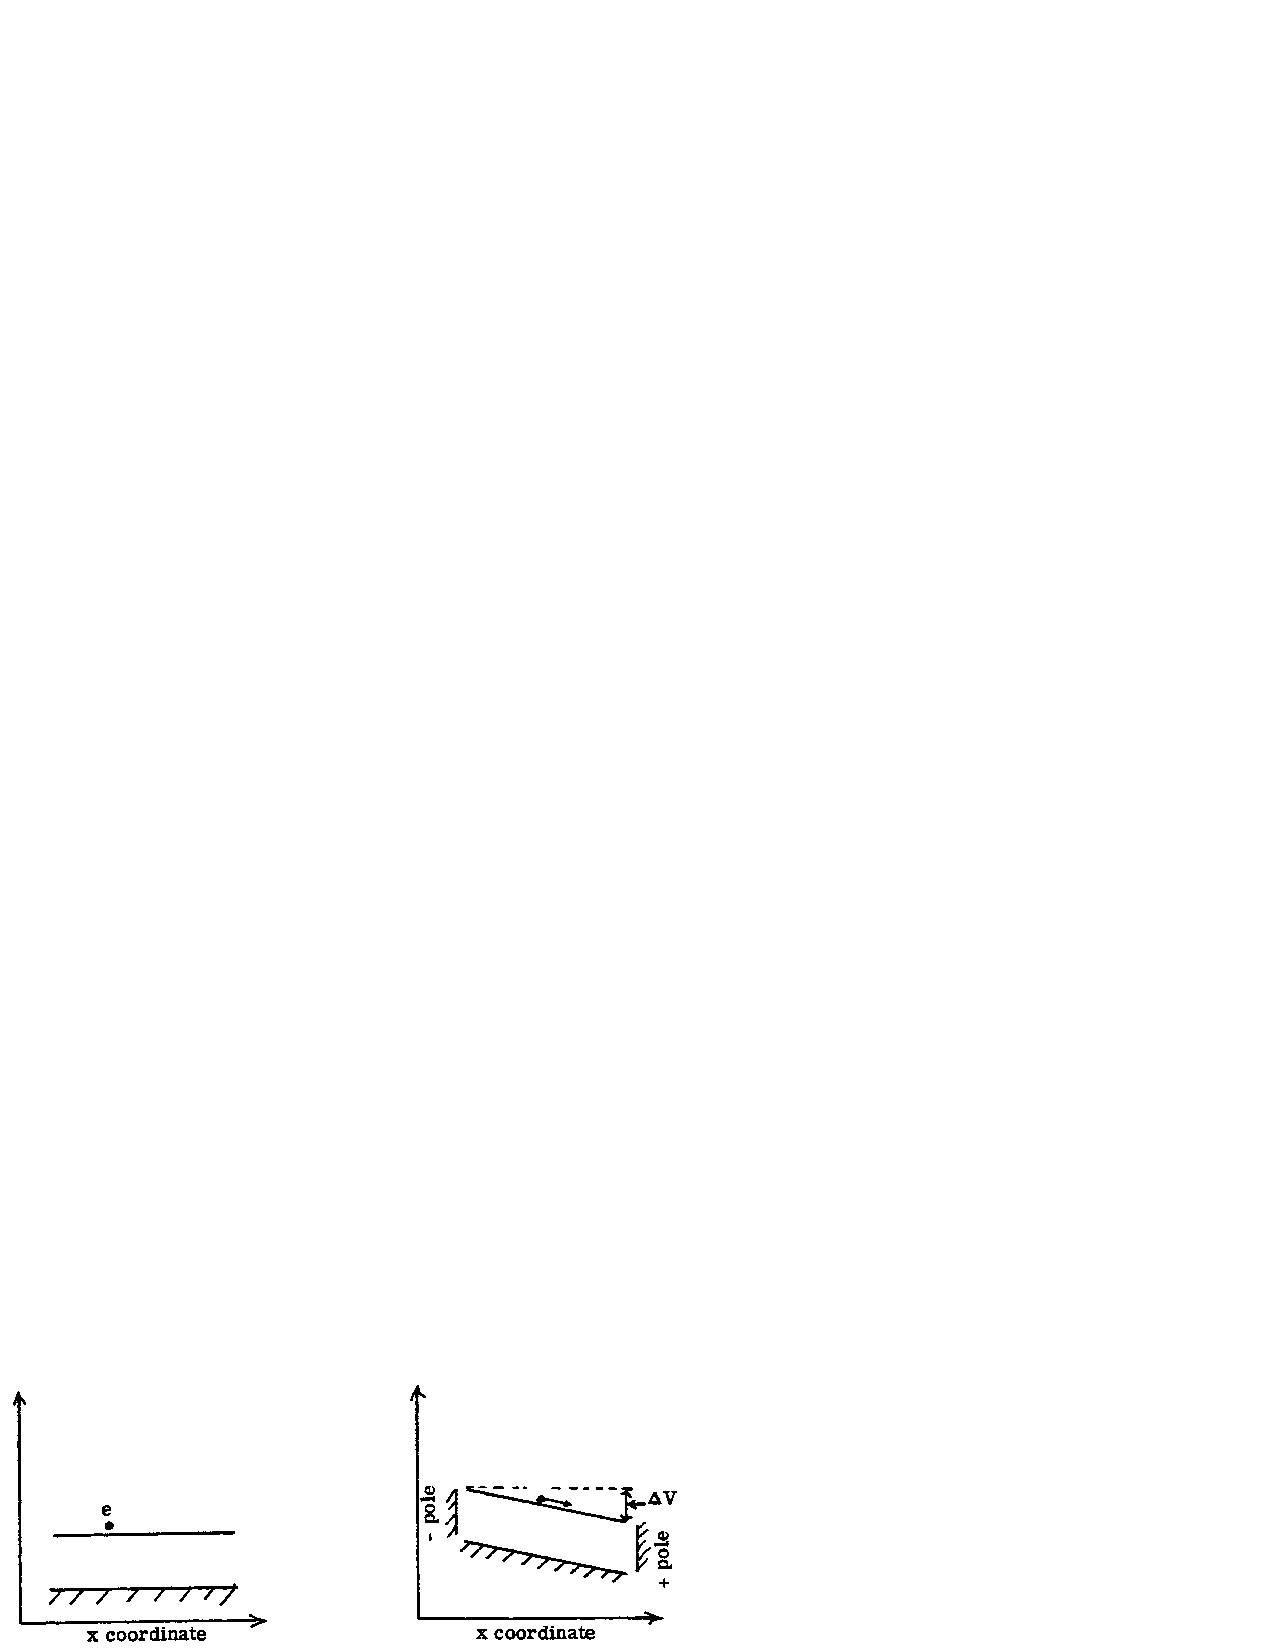
\includegraphics[scale=0.75]{fg8-09}
\end{center}
\caption{Semiconductor with (a) no electric field and (b) an applied
electric field equal to $\Delta V$.}
\label{chap8-fig9}
\end{figure}

Similarly, if one electron is missing from the valence 
band, application of the electron field will cause the remaining electrons 
to move toward the positive pole by populating the unfilled
orbital. You can think of the missing electron as having been removed from 
an Si-Si bond, leaving just one electron in the bond pair and a net positive 
charge as in Figure \ref{chap8-fig10}.

\begin{figure}
\begin{center}
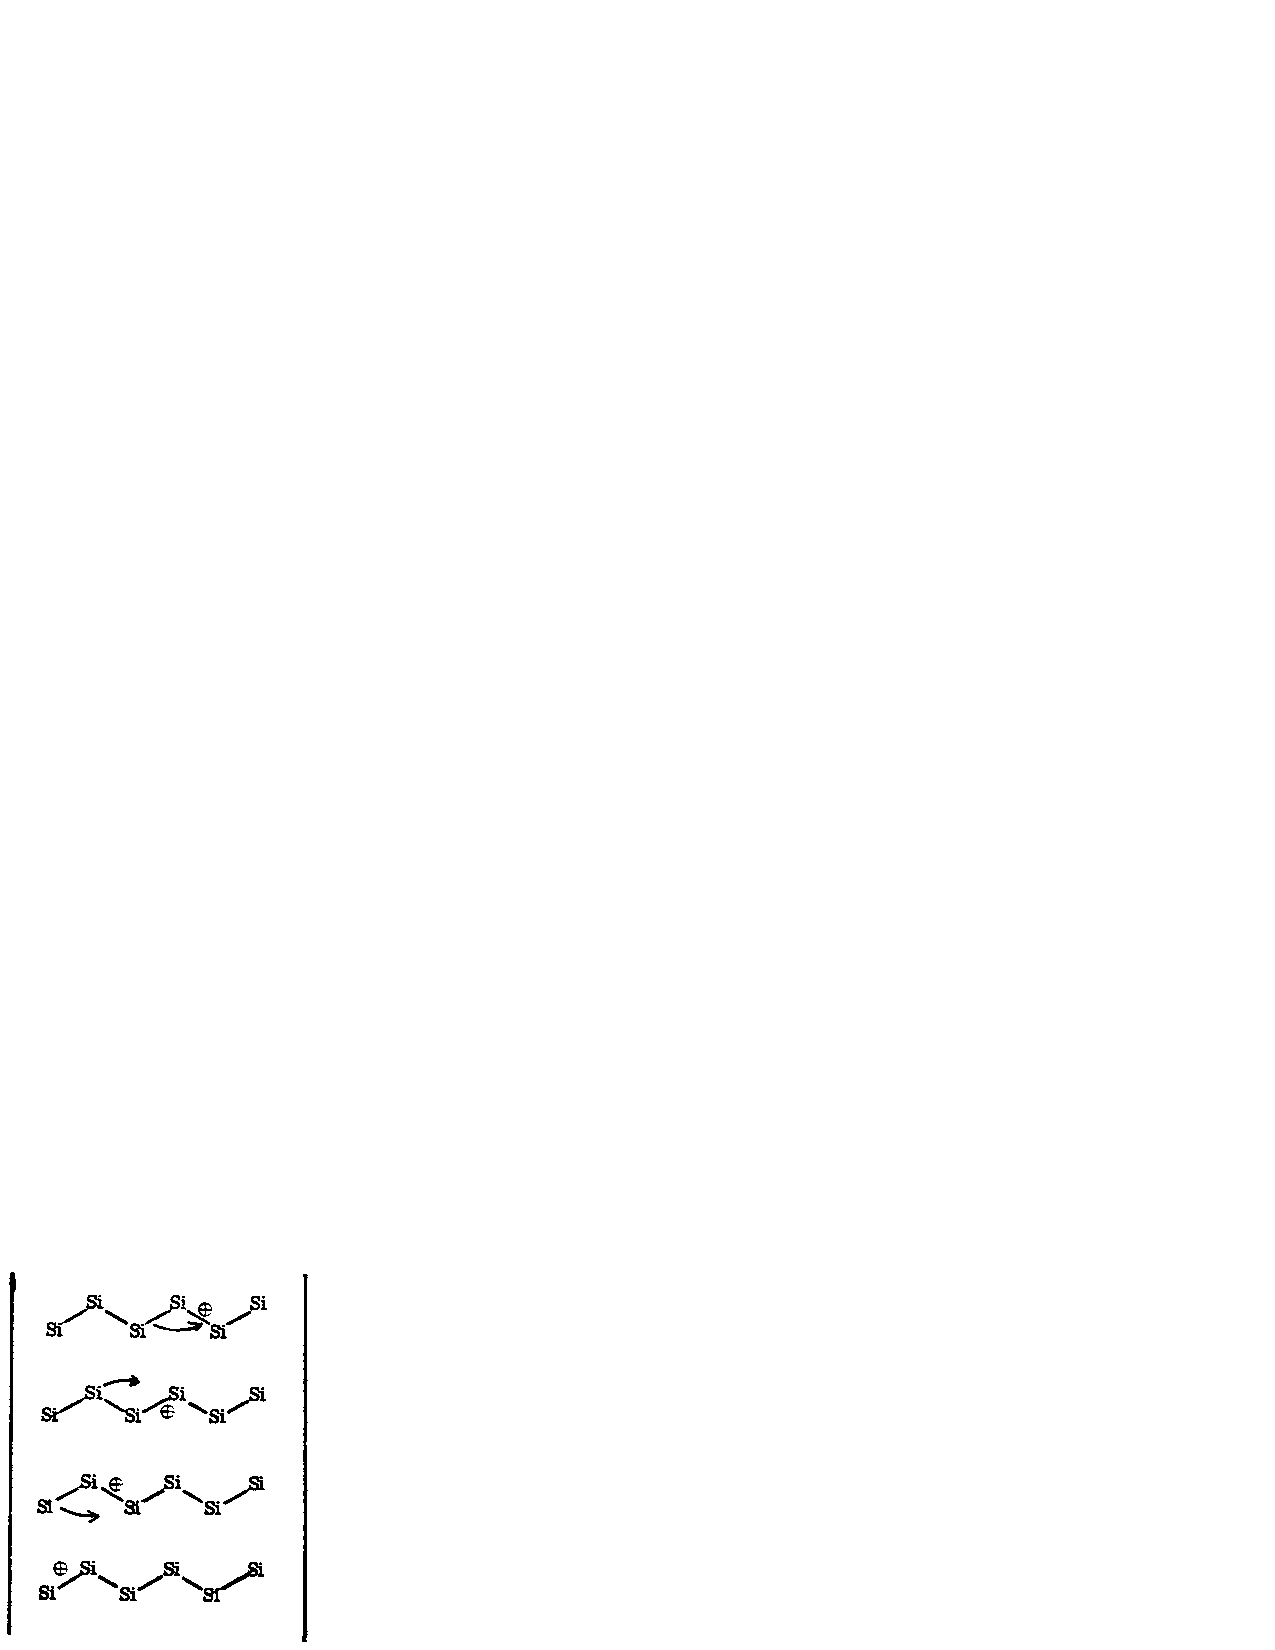
\includegraphics[scale=0.75]{fg8-10}
\end{center}
\caption{Illustration showing how movement of valence band electrons 
to the right appears to cause a plus charge to move towards the left.}
\label{chap8-fig10}
\end{figure}

When the field is applied, as in Figure \ref{chap8-fig9}(b) with the
plus pole to the right, the motion of the electrons to the right leads
to a movement of the net plus charge to the left.  In this case, it is
simpler to follow the motion of the hole, the partially occupied
orbital, rather than the electrons.  This hole moves toward the minus
pole, as good plus charges should, and in the energy diagram the hole
seems to be moving uphill, because the electrons move down hill, as
shown in Figure \ref{chap8-fig11}.

\begin{figure}
\begin{center}
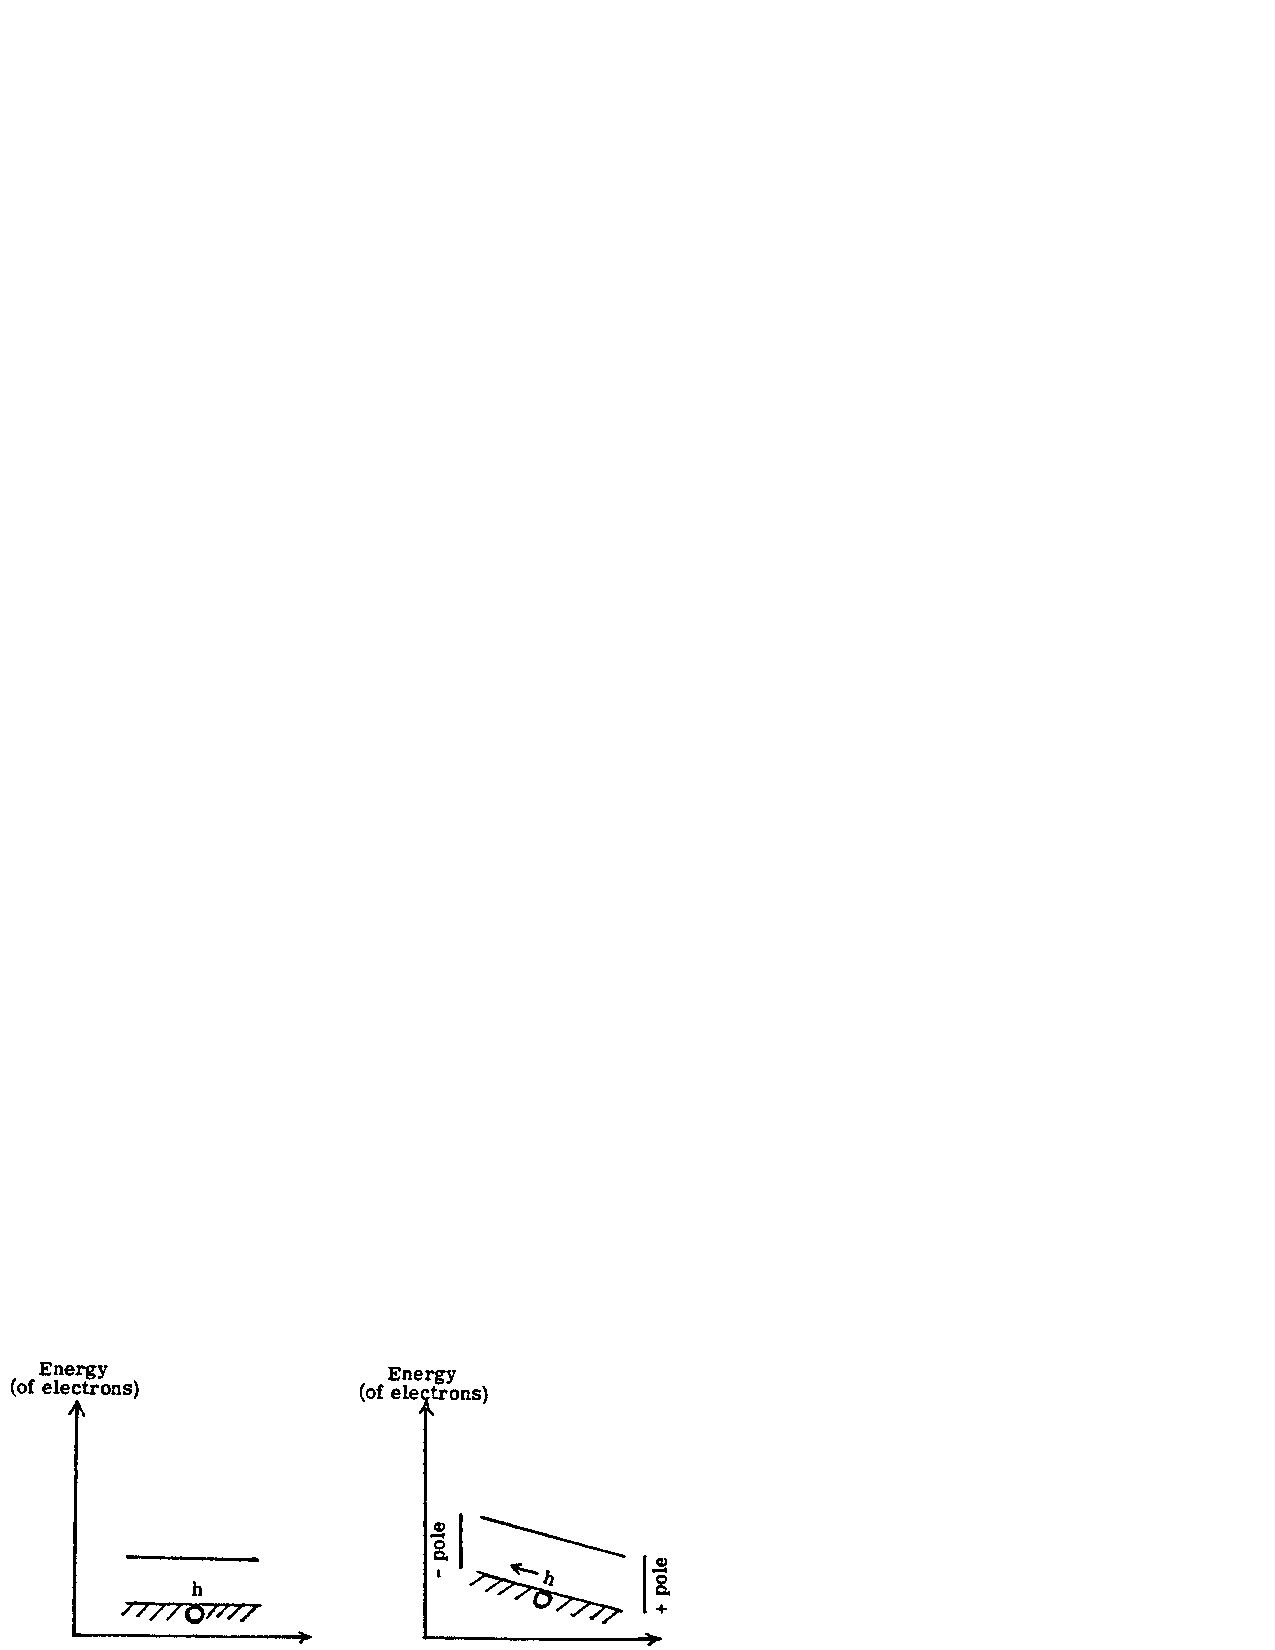
\includegraphics[scale=0.75]{fg8-11}
\end{center}
\caption{A semiconductor system with a hole impurity with (a) no
electric field and (b) an applied electric field.}
\label{chap8-fig11}
\end{figure}


Conduction of electricity by electrons in the conduction band (as in
Figure \ref{chap8-fig9}) is called \emph{n-type} (conduction by flow
of negative charges).  Whereas flow of electricity via electrons
(i.e., holes) in the valence band is called \emph{p-type} (conduction
by flow of positive charges. To excite an electron from the valence
band to the conduction band costs $E_{gap}$ of energy, 1.1 eV for Si,
and leads to two charge carriers, the new electron in the conduction
band and the new hole in the valence band.

From thermodynamics the probability of the system being excited by an 
energy $E$ is proportional to
\begin{equation}
e^{-{E \over kT}} ,
\end{equation}
where $T$ is the temperature in $^{\circ}$K, and $k = 8.6173 10^{-5}$ 
eV/K.  Letting $n$ and $p$ be the concentration, number per cc, of electrons 
and holes, thermodynamic considerations lead to an equilibrium constant,
\begin{equation}
np = Ae^{{E_{gap} \over kT}} ,
\end{equation}
where $A$ depends only weakly upon temperature.  For the perfect crystal,
\begin{equation}
n = p - \sqrt{A} e^{{E_{gap} \over 2kT}} ,
\end{equation}
the conductivity is proportional to $n + p$, leading to
\begin{equation}
\sigma = \sigma_0 e^{-{E_{gap} \over 2kT}} ,
\end{equation}
or a resistivity of
\begin{equation}
\rho = {1 \over \sigma} = \rho_0 e^{{E_{gap} \over 2kT}} ,
\end{equation}
as indicated in Figure \ref{chap8-fig12}.


\begin{figure}
\begin{center}
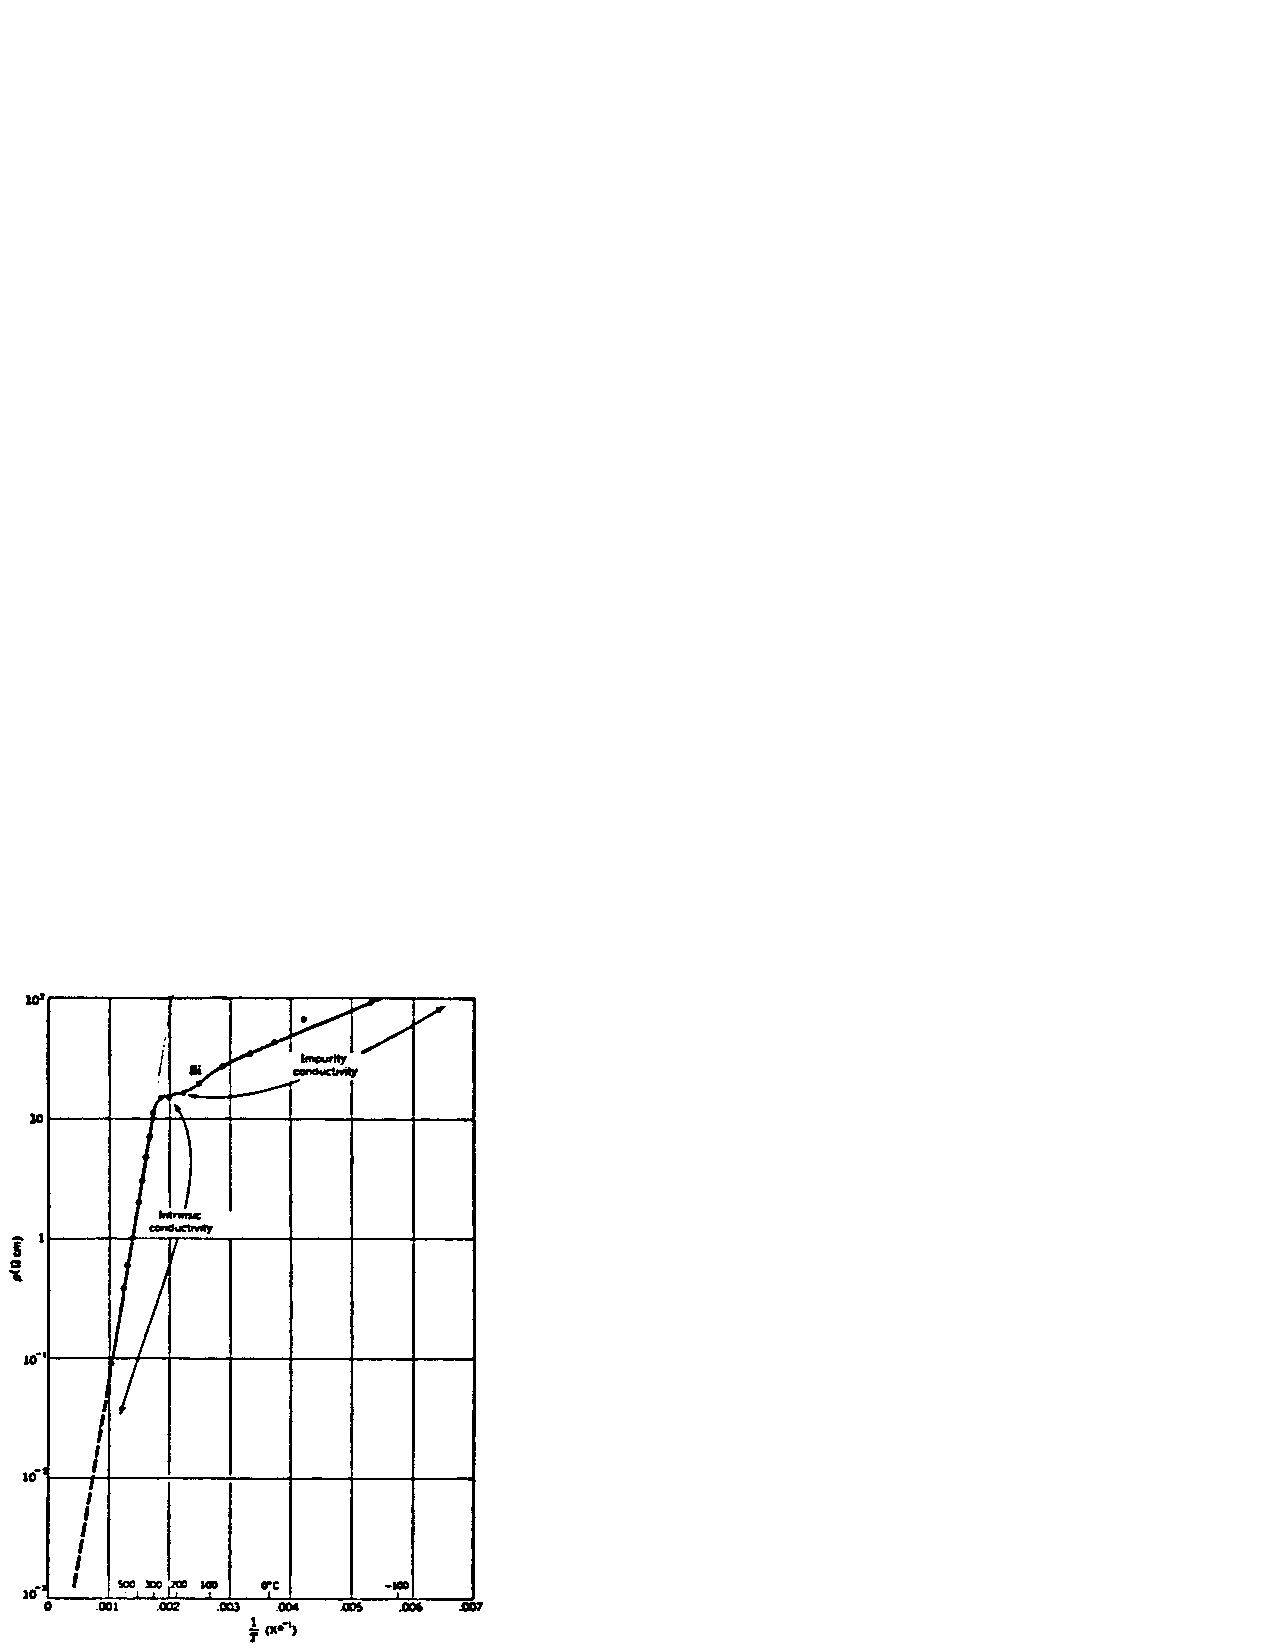
\includegraphics[scale=0.75]{fg8-12}
\end{center}
\caption{The electrical conductivity of pure silicon as a function of
temperature, illustrating the exponential variation of conductivity
with $1/T$.} 
\label{chap8-fig12}
\end{figure}

As $T$ is increased, there are more and more electrons excited from the 
valence band to the conduction band, and the conductivity increases 
exponentially.  This provides a simple way to experimentally determine 
the energy gap.  However, for sufficiently small temperatures, this
conductivity becomes so small that other sources of charge carriers, due to 
impurities or imperfections, become dominant, as indicated in Figure 
\ref{chap8-fig12}. Systems where conduction is dominated by thermal excitation of 
electrons from the valence band to the conduction band, as discussed,
are called {\it intrinsic} semiconductors. The case of impurity
conduction will be discussed next.

\subsection{Impurity Conduction in Si}

Consider the case in which one Si atom of crystalline Si is replaced
by a P atom (this is called a \emph{substitutional} impurity). The
main effect here is that the P has one more electron than the Si it
replaces, leading to the situation sketched in Figure
\ref{chap8-fig13}(a).

\begin{figure}
\begin{center}
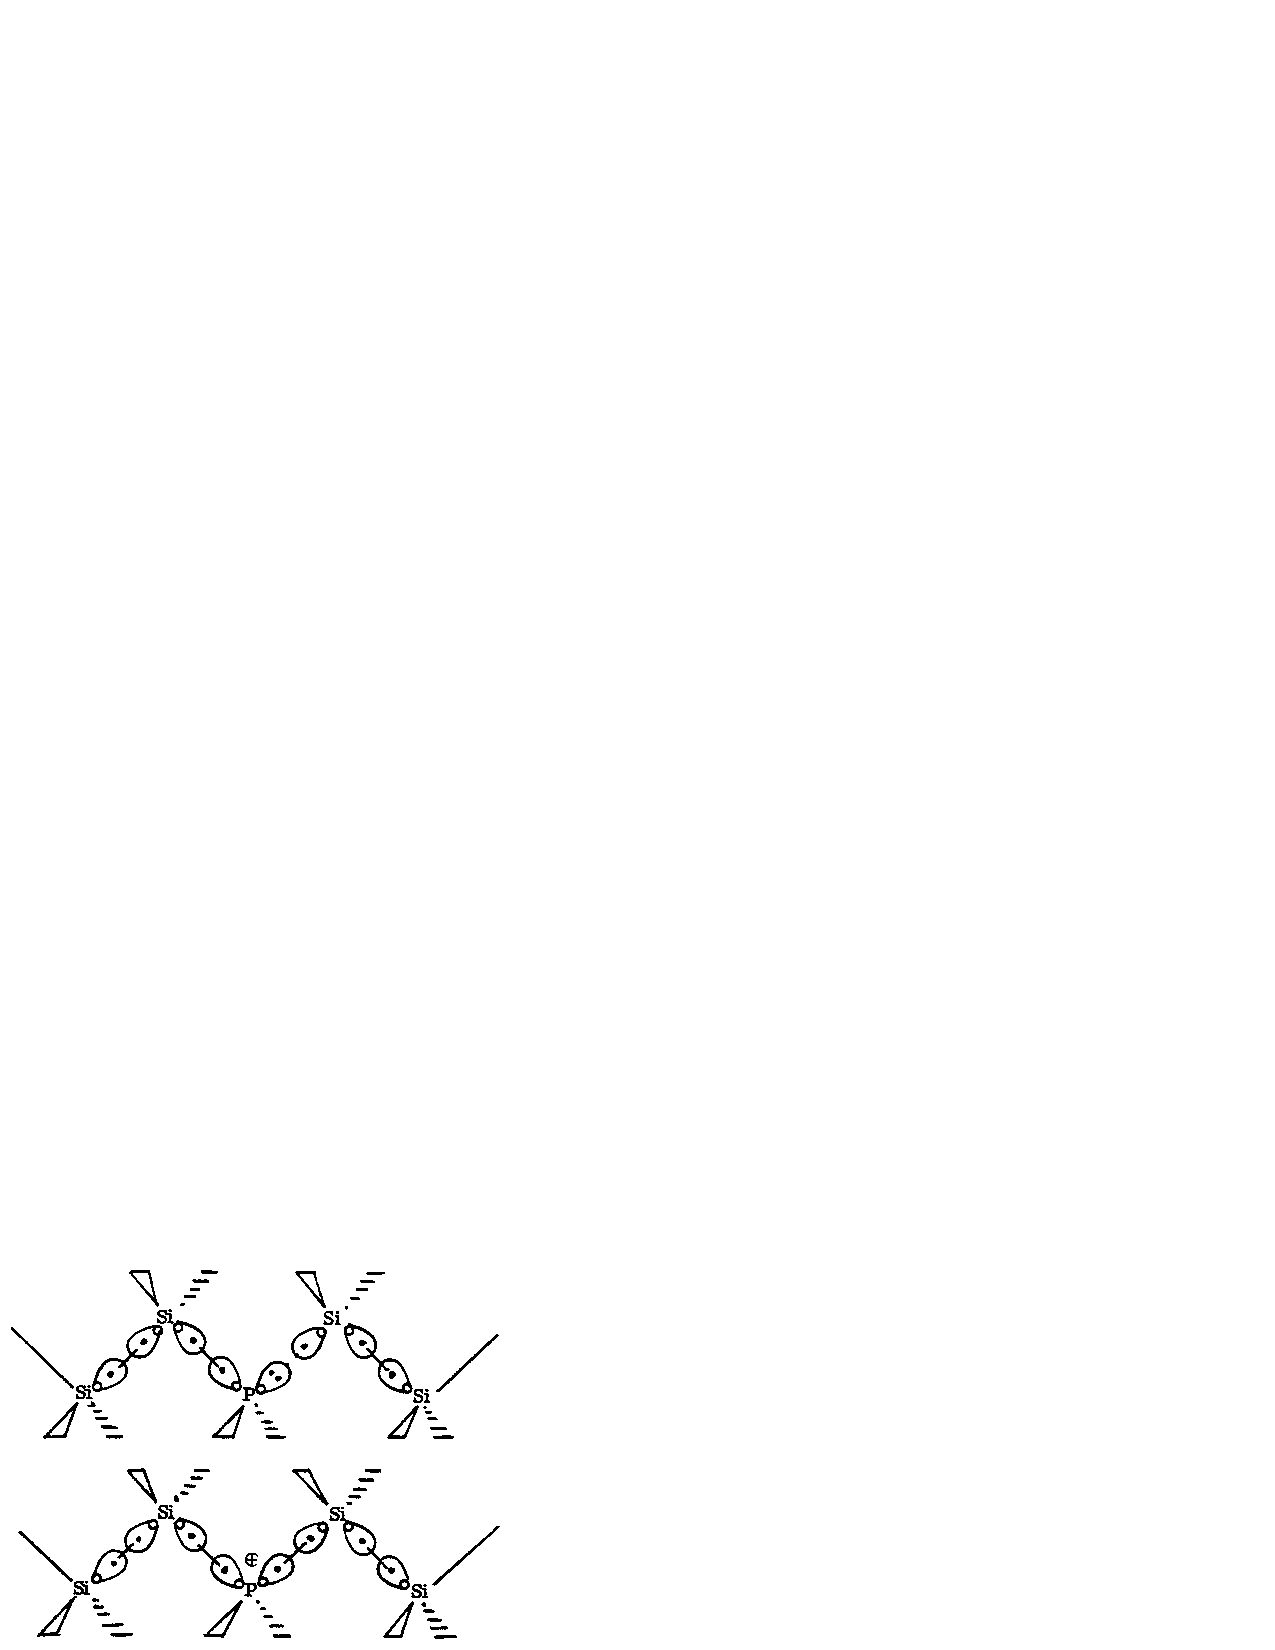
\includegraphics[scale=0.75]{fg8-13}
\end{center}
\caption{}
\label{chap8-fig13}
\end{figure}

The P can make covalent bonds to three of its four Si neighbors;
however, there is an extra electron in the way of making the fourth
bond.  As a result, it is very easy to remove this extra electron,
donating it into the conduction band. This leaves behind a P making
covalent bonds to all four of its neighbors but a residual positive
charge. This energy to ionize the P impurity is only 0.044 eV, putting
the electron into the conduction band, and hence, at room temperature
a large fraction of such P impurities are ionized. This leads to a
number of charge carriers in the conduction band directly proportional
to the number of P impurities.  Thus, one can deliberately add some
specific concentration of P to the Si in order to achieve a specific
concentration of electrons in the conduction band, and we refer to P
as an \emph{n-type dopant} or as a \emph{donor impurity}.

Similarly, replacement of Si by Al or Ga, leads to the situation in
Figure \ref{chap8-fig14}(a), where there is one too few electrons for
the fourth bond to the Al. As a result, the Al site is quite willing
to accept an additional electron to provide a fourth bond, as in
Figure \ref{chap8-fig14}(b). This leads to a net negative charge in
the region of the Al. Indeed, it costs only 0.067 eV to remove an
electron from the valence band, at some remote site in the crystal,
and to add it to the Al site as in Figure \ref{chap8-fig14}(b).  This
leads to a hole in the valence band, and we refer to Al as a
\emph{p-type dopant} or as an \emph{acceptor impurity}.
\begin{figure}
\begin{center}
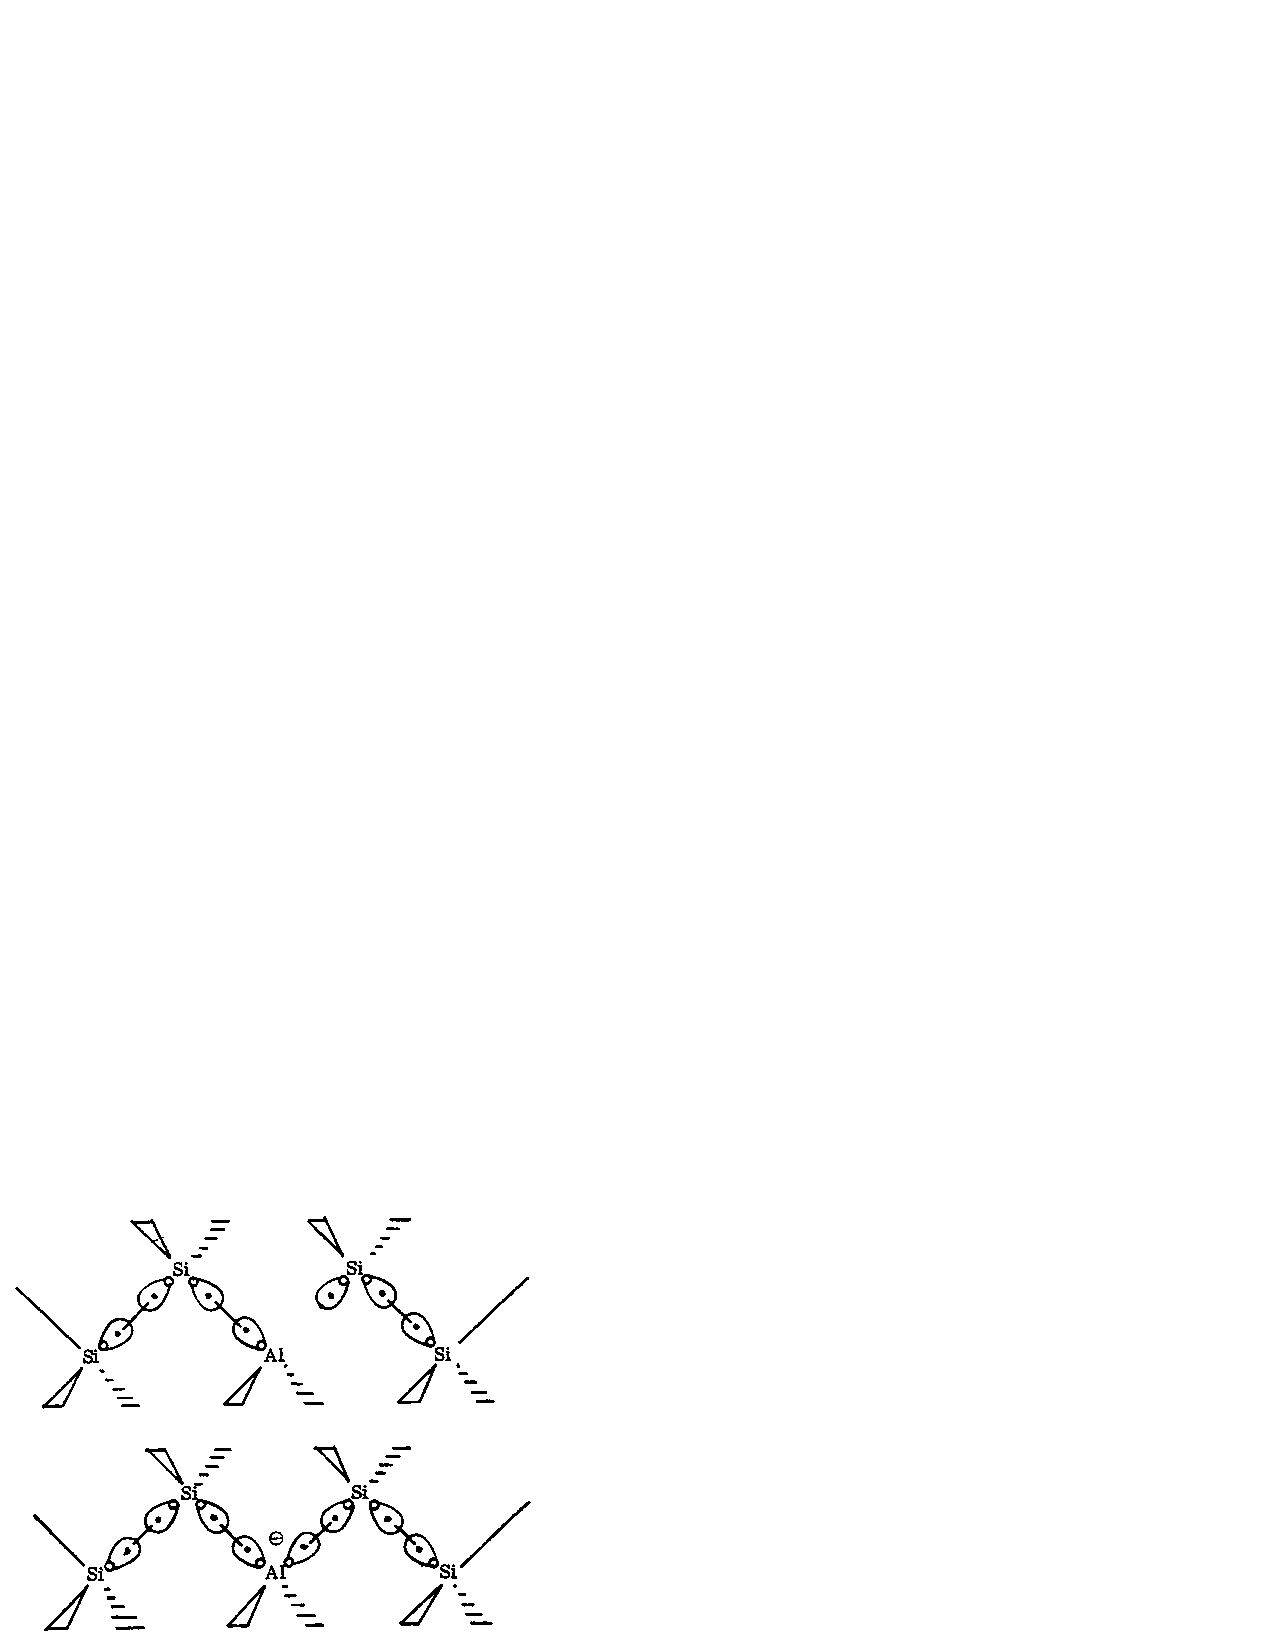
\includegraphics[scale=0.75]{fg8-14}
\end{center}
\caption{}
\label{chap8-fig14}
\end{figure}

Even small concentrations, one part in 10$^6$ to one part in 10$^3$, 
of donor or acceptor impurities can lead to dramatic changes in the 
conduction properties.   Indeed, variations on such themes are the basis 
of the remarkable revolution in electronic devices over the last two
decades.

Comparing diamond, Si, Ge, and $\alpha$-Sn, the nonmetallic form of Sn
stable at low temperatures, as in Table \ref{chap8-tab7}, we find a
dramatic decrease in energy gap upon going to the heavy elements,
basically there is less difference in energy between bonding and
antibonding levels.  In all cases, donor levels can be found in group
V, N, P, As, and Sb, and acceptor levels can be found in group III, B,
Al, Ga, and In. Some of the energies to ionize such impurities are
listed in Table \ref{chap8-tab8}.  To obtain good substitutional
impurities one wants similar sizes.  Thus, B and N are more
appropriate for diamond, whereas In and Sb would be more appropriate
for $\alpha$-Sn.  For $\alpha$-Sn the smaller impurities, N and B,
would probably go into other sites, e.g., interstitial sites
corresponding to positions in between the normal tetrahedral
locations.

\begin{table}
\caption{Energy gaps for semiconductors based on diamond structure.$^a$}
\label{chap8-tab7}
\begin{tabular}{cccc}\\ \hline
& Energy$^b$ Gap (eV) & Lattice Parameter\cr
& Reference d & Reference a\cr

Diamond & 5.48 & 5.4 & 3.560\cr
SiC & 2.2$^c$ & & 4. 348$^e$\cr
Si & 1.110 & 1.107 & 5.431\cr
Ge & 0.664 & 0.67 & 5.658\cr
$\alpha$-Sn & 0 & 0.08 & 6.491\cr
BN & 6$-$8 & $\sim$4 & 3.615\cr
AlP & 2.45 & 2.5 & 5.451\cr
GaAs & 1.426 & 1.35 & 5.653\cr
InSb & 0.180 & 0.165 & 6.479\cr
\hline
\end{tabular}\\
$^a$ From the CRC Handbook of Chemistry and Physics, 60th 
Edition, page E-102. 
$^b$ Minimum gap at room temperature. 
$^c$ The most stable SiC, 6H or $\alpha$-SiC type II, has $E_g = 
2.86$ eV. 
$^d$ LB Tables, volume M/17a, 1982. 
$^e$ Wyckoff, {\it loc. cit}.
\end{table}

\begin{table}
\caption{Ionization energies, in eV, for substitutional 
impurity levels in diamond structure semiconductors.}
\label{chap8-tab8}
\begin{tabular}{ccccc}\\ \hline

Impurity & Type & C$^a$ & Si$^b$ & Ge$^c$\cr

N & D & $\sim$2. & 0.14\cr
P & D & & O.0453 & 0.01289\cr
As & D & & 0.0538 & 0.01417\cr
Sb & D & & 0.0428 & 0.01032\cr
Bi & D & & 0.069 & 0.01281\cr
B & A & 0.37 & 0.045 & 0.01087\cr
Al & A & & 0.067 & 0.01115\cr
Ga & A & & 0.074 & 0.01132\cr
In & A & & 0.153 & 0.01199\cr
T1 & A & & 0.25 & 0.01345\cr
\hline
\end{tabular}\\
$^a$ Landolt-Bornstein Tables IM/17a (1982). 
$^b$ {\it Ibid}. page 48.
$^c$ {\it Ibid}. page 87.
\end{table}

\subsection{III-V Compounds}

As indicated in Table \ref{chap8-tab4}, the energy gaps of the III-V
systems are larger than for the group IV system in the same row.

From Figure \ref{chap8-fig15} we see that substituting Se for As leads
to a donor impurity, while substituting Ge for As leads to an acceptor
bond.  Similarly, substituting Zn for Ga leads to an acceptor bond,
while substituting Ge for Ga leads to a donor bond. These cases are
illustrated in Figure \ref{chap8-fig15}, and the energy levels for
various cases are in Table \ref{chap8-tab9}.

\begin{table}
\caption{Ionization energies, in eV, for substitutional 
impurity levels of GaAs.$^a$}
\label{chap8-tab9}
\begin{tabular}{ccc}\\ \hline

& Ga Site & As Site\cr

Be & 0.0280 A\cr
Mg & 0.0288 A\cr
Zn & 0.0307 A\cr
Cd & 0.0347 A\cr
C & 0.005913 D & 0.0270 A\cr
Si & 0.005839 D & 0.0348 A\cr
Ge & 0.005882 D & 0.0404 A\cr
Sn & & 0.167 A\cr
S & & 0.005870 D\cr
Se & & 0.005789 D\cr
Mn & 0.113 A\cr
\hline
\end{tabular}\\
$^a$ LB Tables III/17a, page 224.
\end{table}

\begin{figure}
\begin{center}
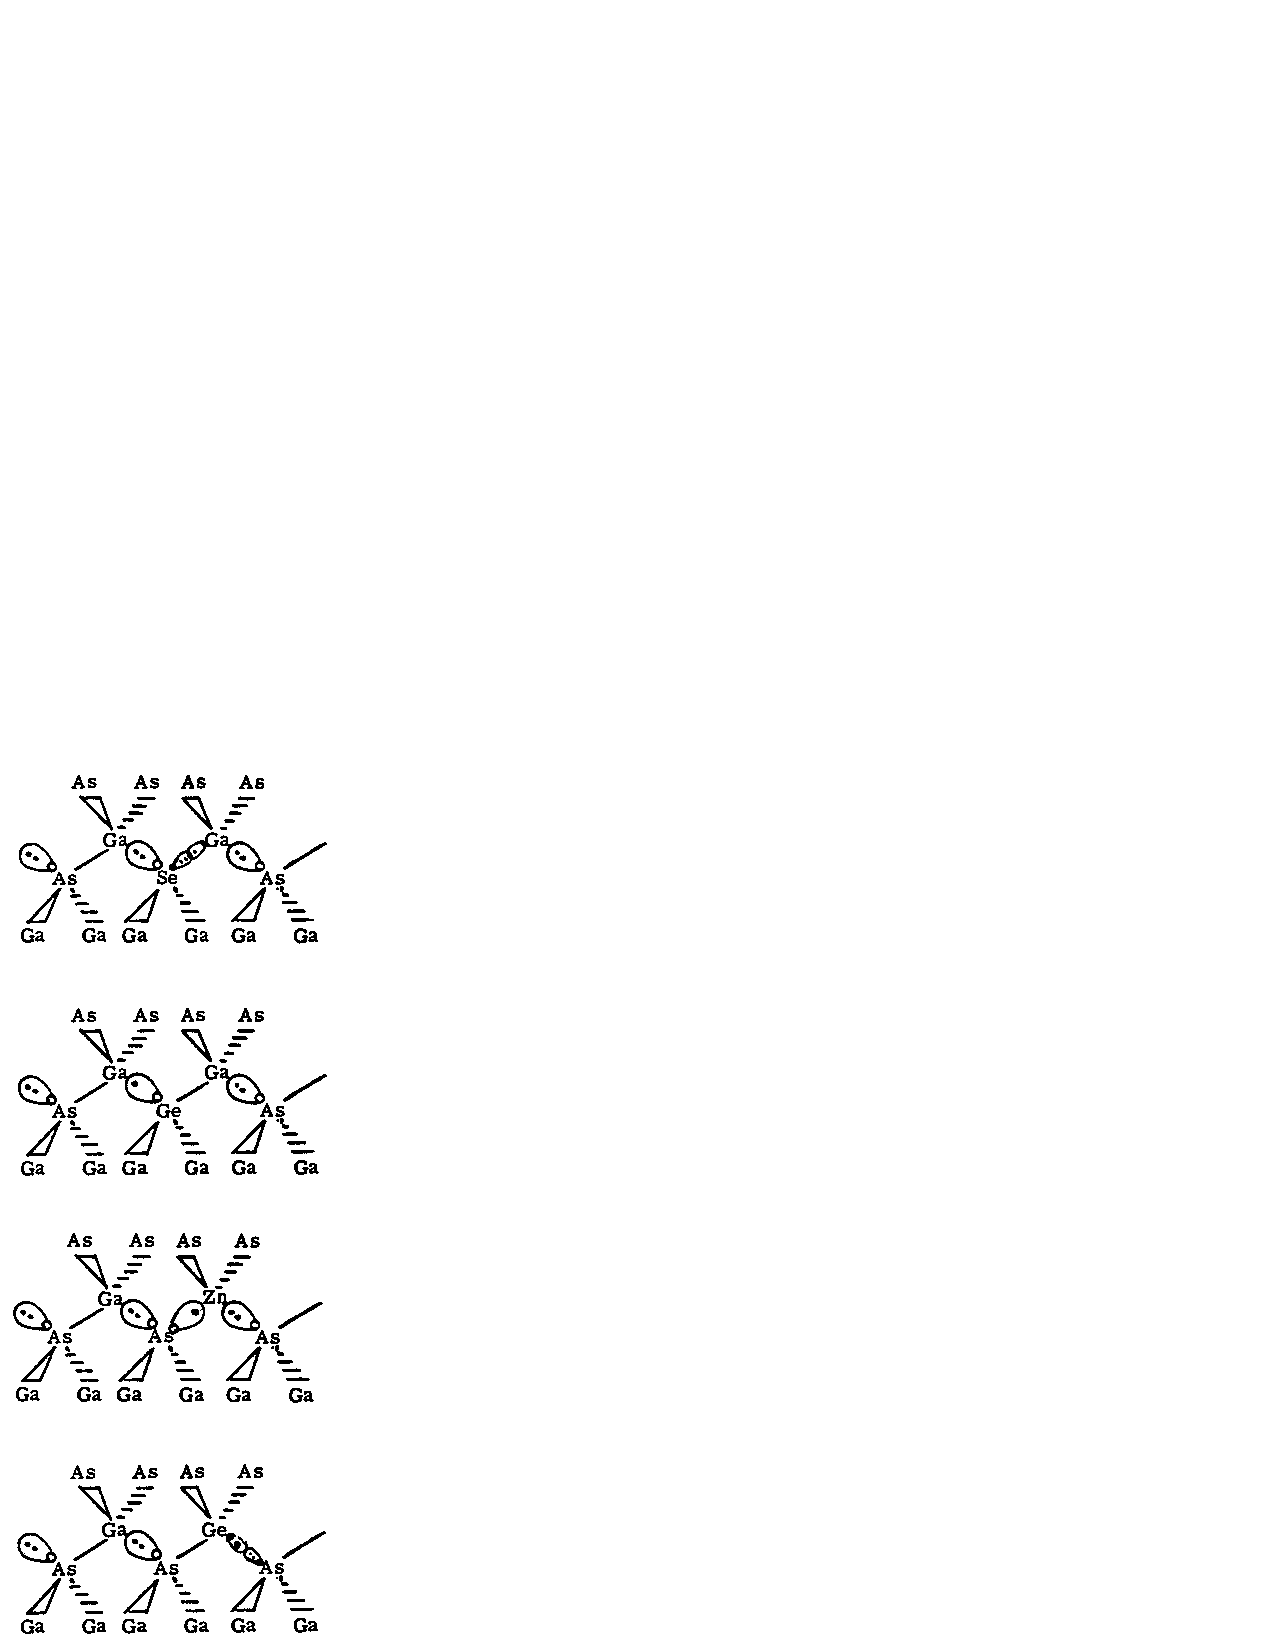
\includegraphics[scale=0.75]{fg8-15}
\end{center}
\caption{Substitutional impurities in GaAs: (i) Se/As (donor), (ii)
Ge/As (acceptor), (iii) Zn/Ga (acceptor), (iv) Ge/Ga (donor).}
\label{chap8-fig15}
\end{figure}

\section{Semiconductor Surfaces}

As all good things come eventually to an end, so also must crystals. The 
properties of such crystal surfaces can have a dramatic effect upon the 
properties, and we will consider here some aspects of such surfaces.

Before we get started, there is some notation to discuss. Consider a
crystalline lattice with unit cell dimensions $a$, $b$, and $c$, in
the $x$, $y$, and $z$ directions (not necessarily orthogonal) as in
Figure \ref{chap8-fig16}(a).  Now we pass a plane through a set of
equivalent atoms, i.e., same atom and in identical environment.  A
property of periodic structures, lattices, is that a set of parallel
planes can be passed through all other equivalent atoms and that all
planes of this set are equally spaced.  Another property is that if
one plane passes through the origin, the next plane will intersect the
axes at $a/h$, $b/k$, $c/\ell$, where $hk\ell$ are integers, as
indicated in Figure \ref{chap8-fig16}(b).  

\begin{figure}
\begin{center}
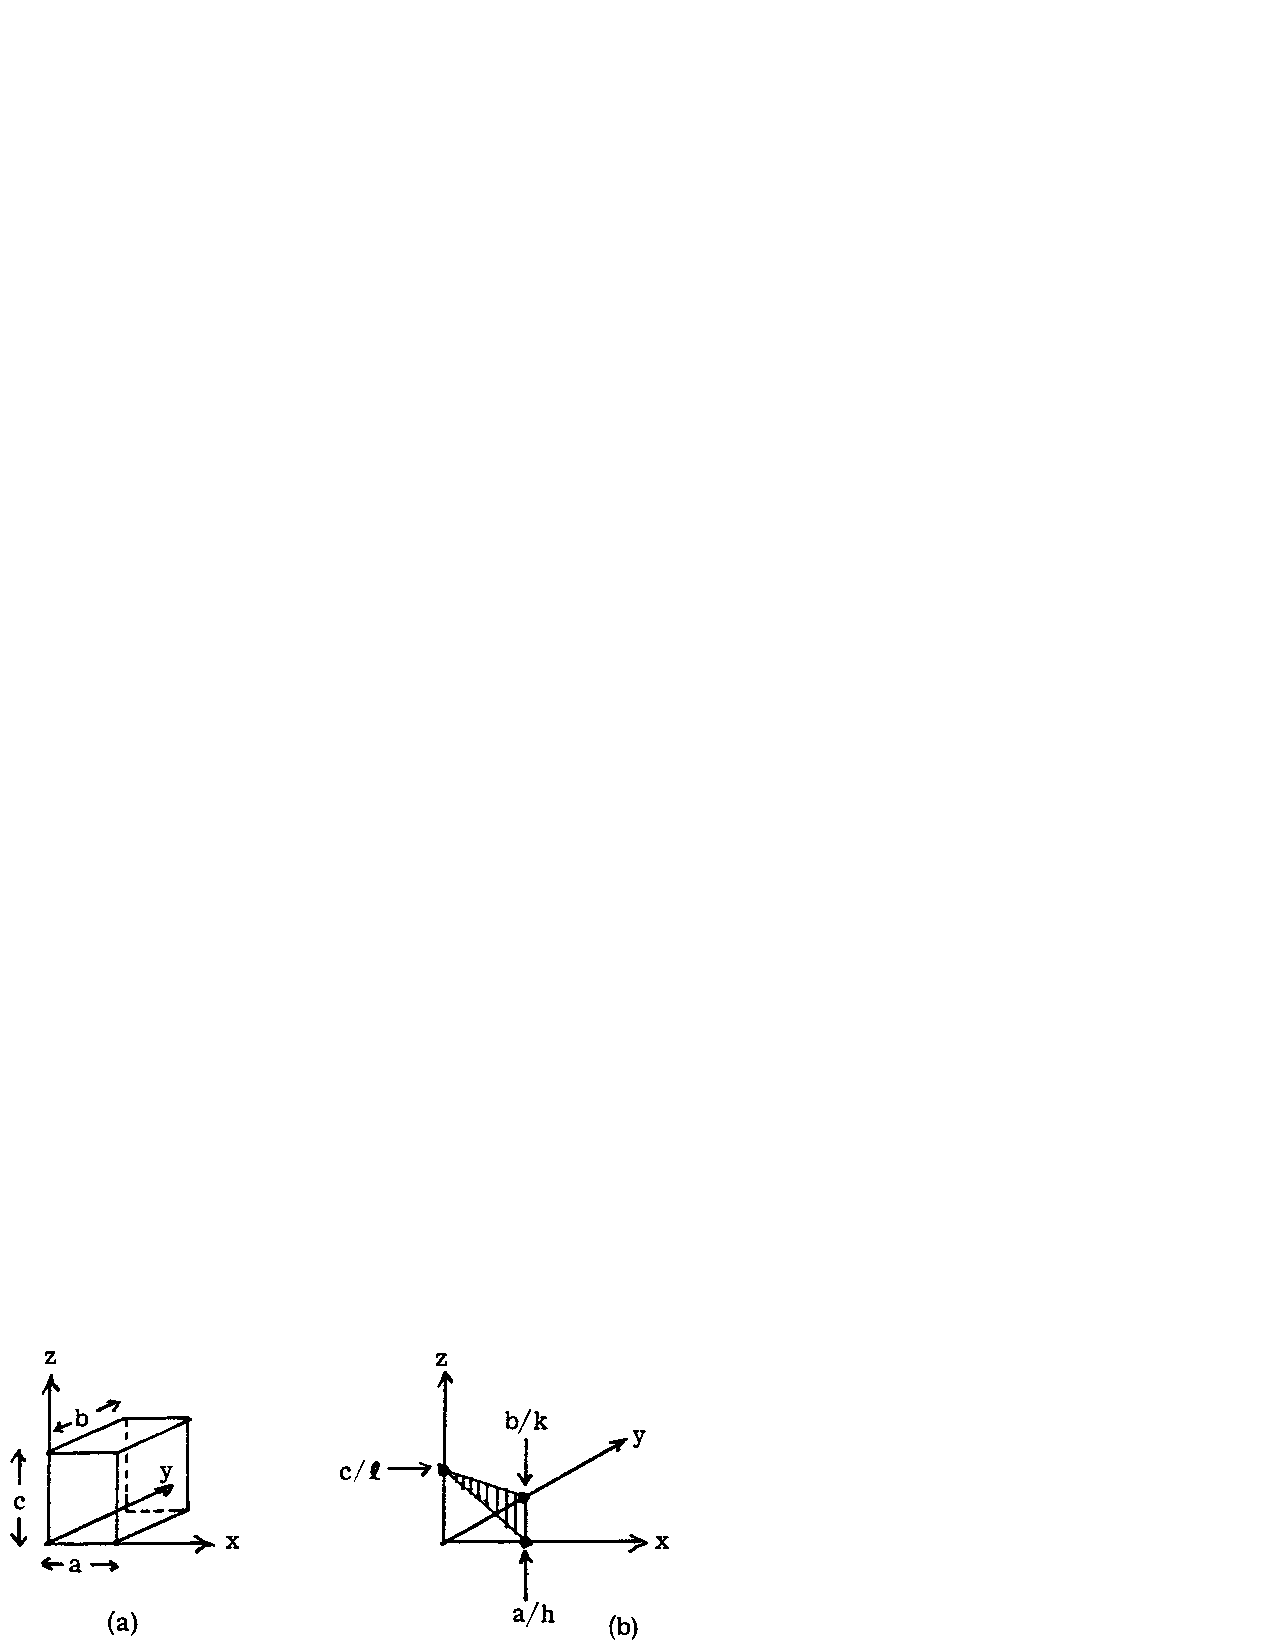
\includegraphics[scale=0.75]{fg8-16}
\end{center}
\caption{}
\label{chap8-fig16}
\end{figure}


Consequently, each set of parallel planes can be denoted simply by the
integers, $hk \ell$, which are called the \emph{Miller indices}. Some
simple examples are given in Figure \ref{chap8-fig17}.

\begin{figure}
\begin{center}
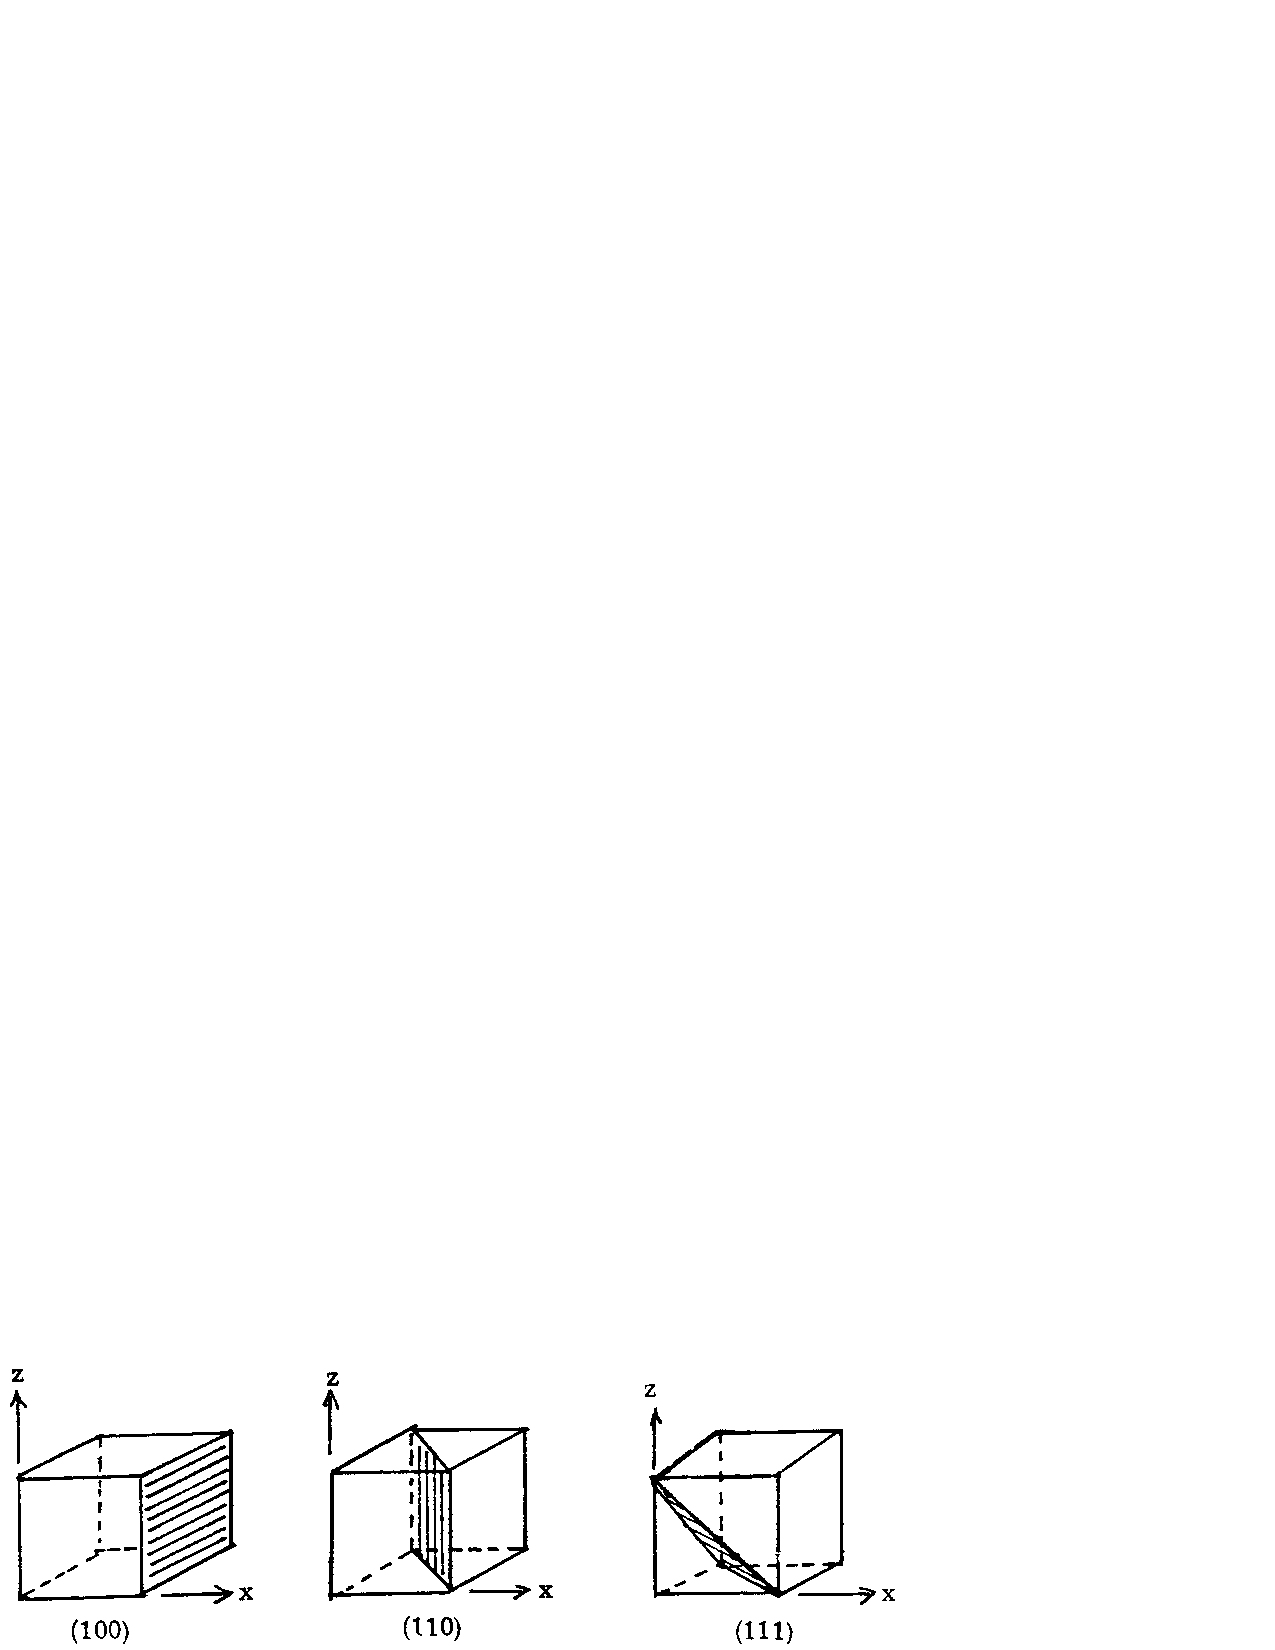
\includegraphics[scale=0.75]{fg8-17}
\end{center}
\caption{}
\label{chap8-fig17}
\end{figure}

The reason that this is useful for surfaces is that most interesting 
surfaces correspond closely to one of these lattice planes, and hence, 
the surface is indicated by $hk \ell$, e.g., we speak of the (111) 
surface or the (110) surface, etc.

\subsection{Si}

Starting with the diamond structure of Figure \ref{chap8-fig3}, there
are three particularly simple surfaces to consider, they are (100),
(110), and (111) surfaces.

\subsubsection{Si (100) Surface}

Using one face of the cubic unit cell leads to the (100) surface of Figure 
\ref{chap8-fig18}, where the outline of the original cube is shown
with dotted lines. 

\begin{figure}
\begin{center}
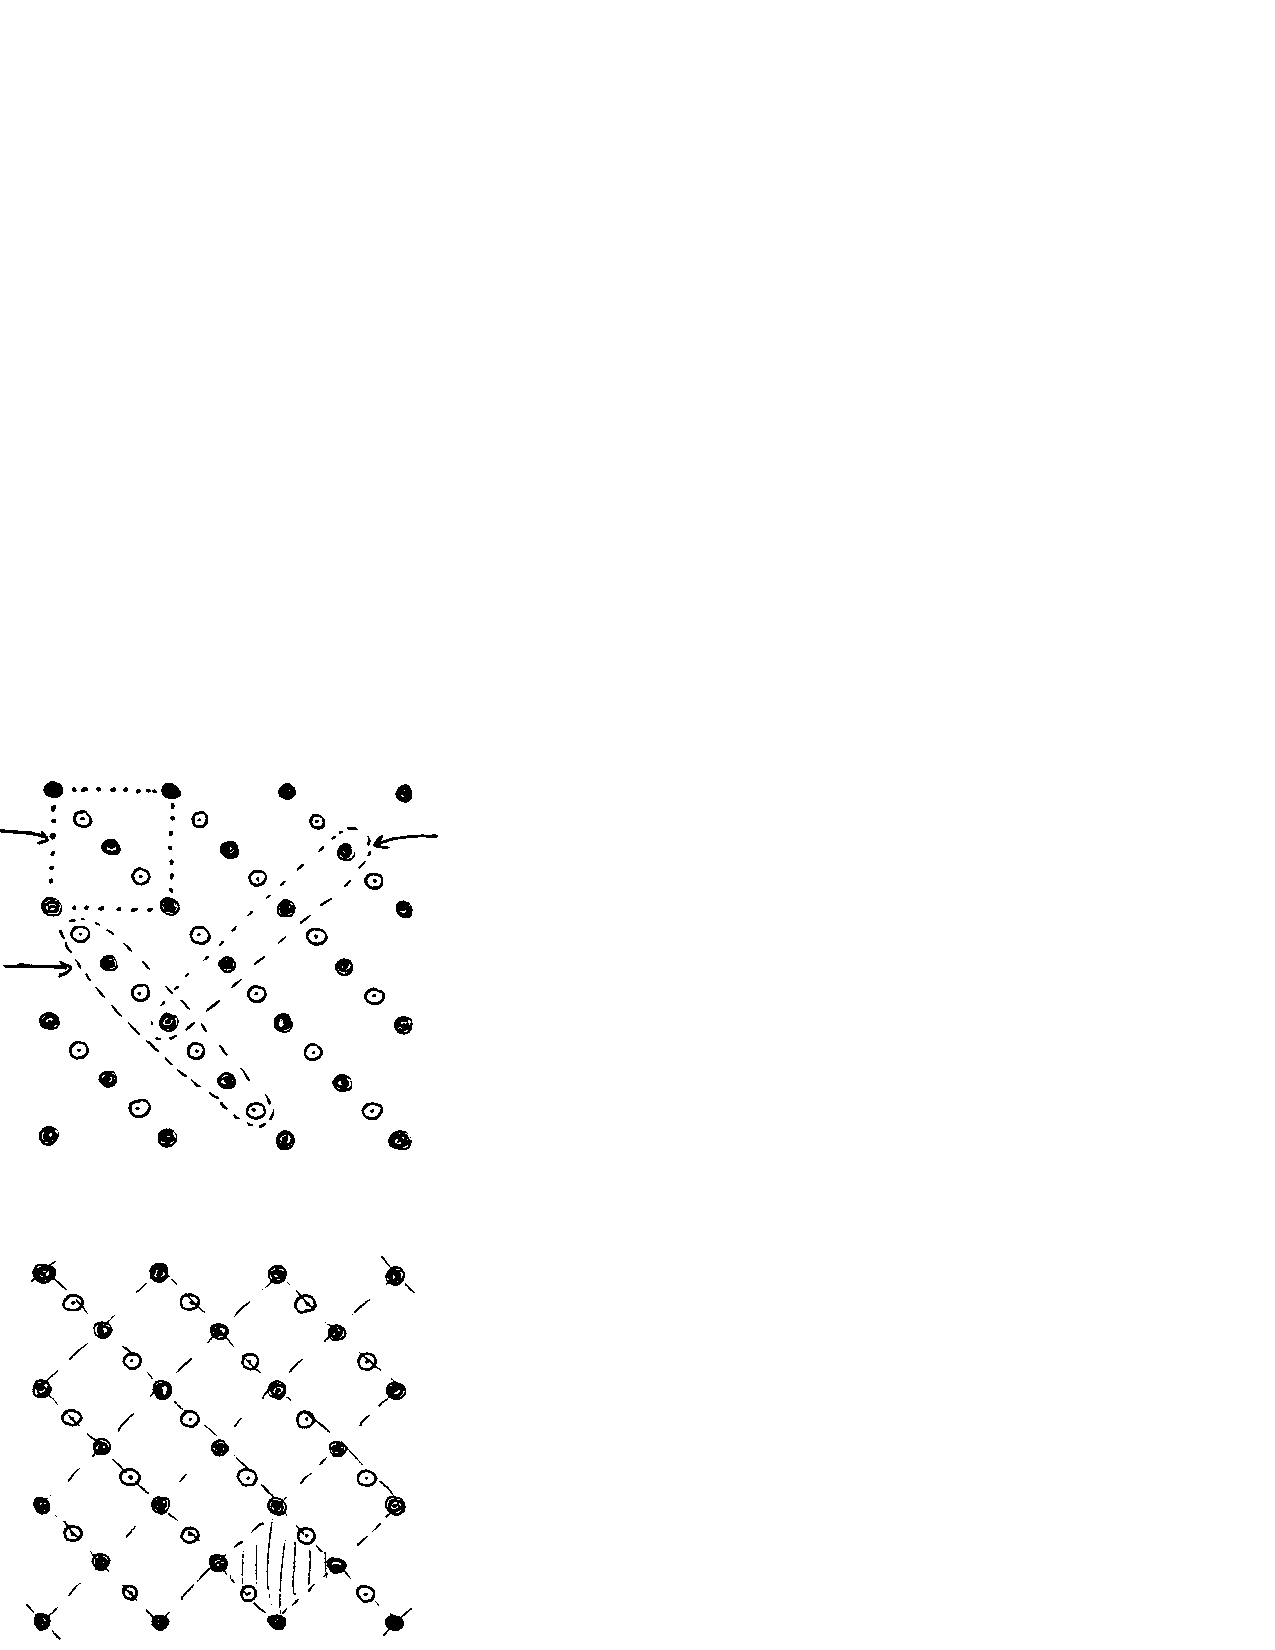
\includegraphics[scale=0.75]{fg8-18}
\end{center}
\caption{$P(1 \times 1)$ unreconstructed surface for Si (100).  Filled
circles are surface atoms, and open circles are subsurface atoms.  The
dotted lines in the top figure indicate the face of the original cubic
unit cell. The surface unit cell is shaded in the bottom figure.}
\label{chap8-fig18}
\end{figure}

In Figure \ref{chap8-fig18}(b), we have shaded a square region that is
referred to as the surface unit cell.  The surface can be divided into
cells identical to this one, making them unit cells, and there is no
smaller cell into which the surface may be divided, making them
primitive unit cells.  Note that the dotted cell at the upper left in
Figure \ref{chap8-fig13}, is a unit cell, but it is not primitive.
Later this cell will be referred to as $P(1 \times 1)$, indicating
that the periodicity is just that expected for the perfect surface, no
reconstruction.

In Figure \ref{chap8-fig18}, we kept each surface atom at the same
position it had in the infinite solid.  However, these surface atoms
will generally change position, the surface reconstructs, since the
bonding is drastically modified from that of the bulk. In order to
understand what sort of reconstruction should be expected, consider
the orbitals on the surface atoms of Figure \ref{chap8-fig18}.  Each
surface atom (solid circles in Figure \ref{chap8-fig18}), is bonded to
two atoms (open circles in Figure \ref{chap8-fig18}) as indicated in
Figure \ref{chap8-fig19}.

\begin{figure}
\begin{center}
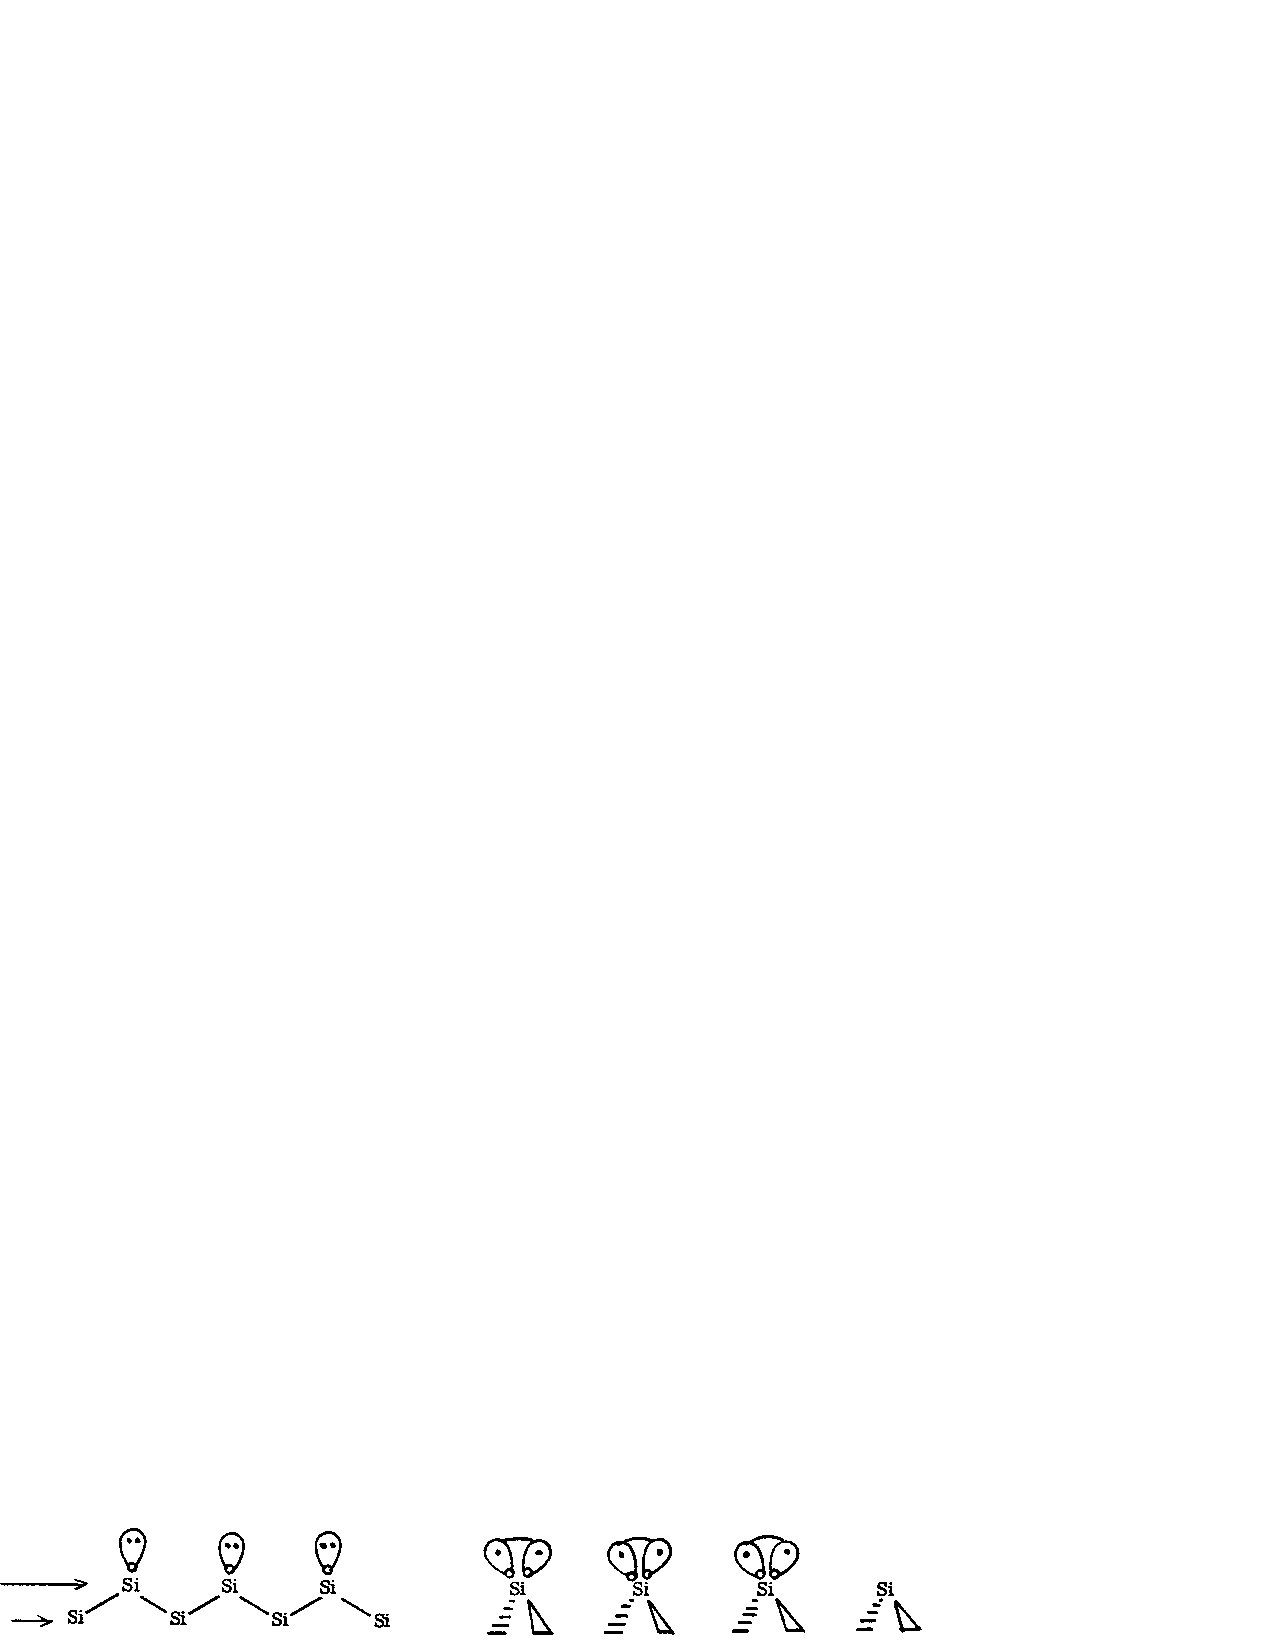
\includegraphics[scale=0.75]{fg8-19}
\end{center}
\caption{Surface Si atoms of (100) surface before reconstruction.}
\label{chap8-fig19}
\end{figure}

Since each surface atom is bonded to only two subsurface atoms, it has
two electrons in nonbonding orbitals.  As a result, the surface atoms
distort, reconstruct, as indicated in Figure \ref{chap8-fig20}, where
the arrows indicate the motion of the surface atoms.


\begin{figure}
\begin{center}
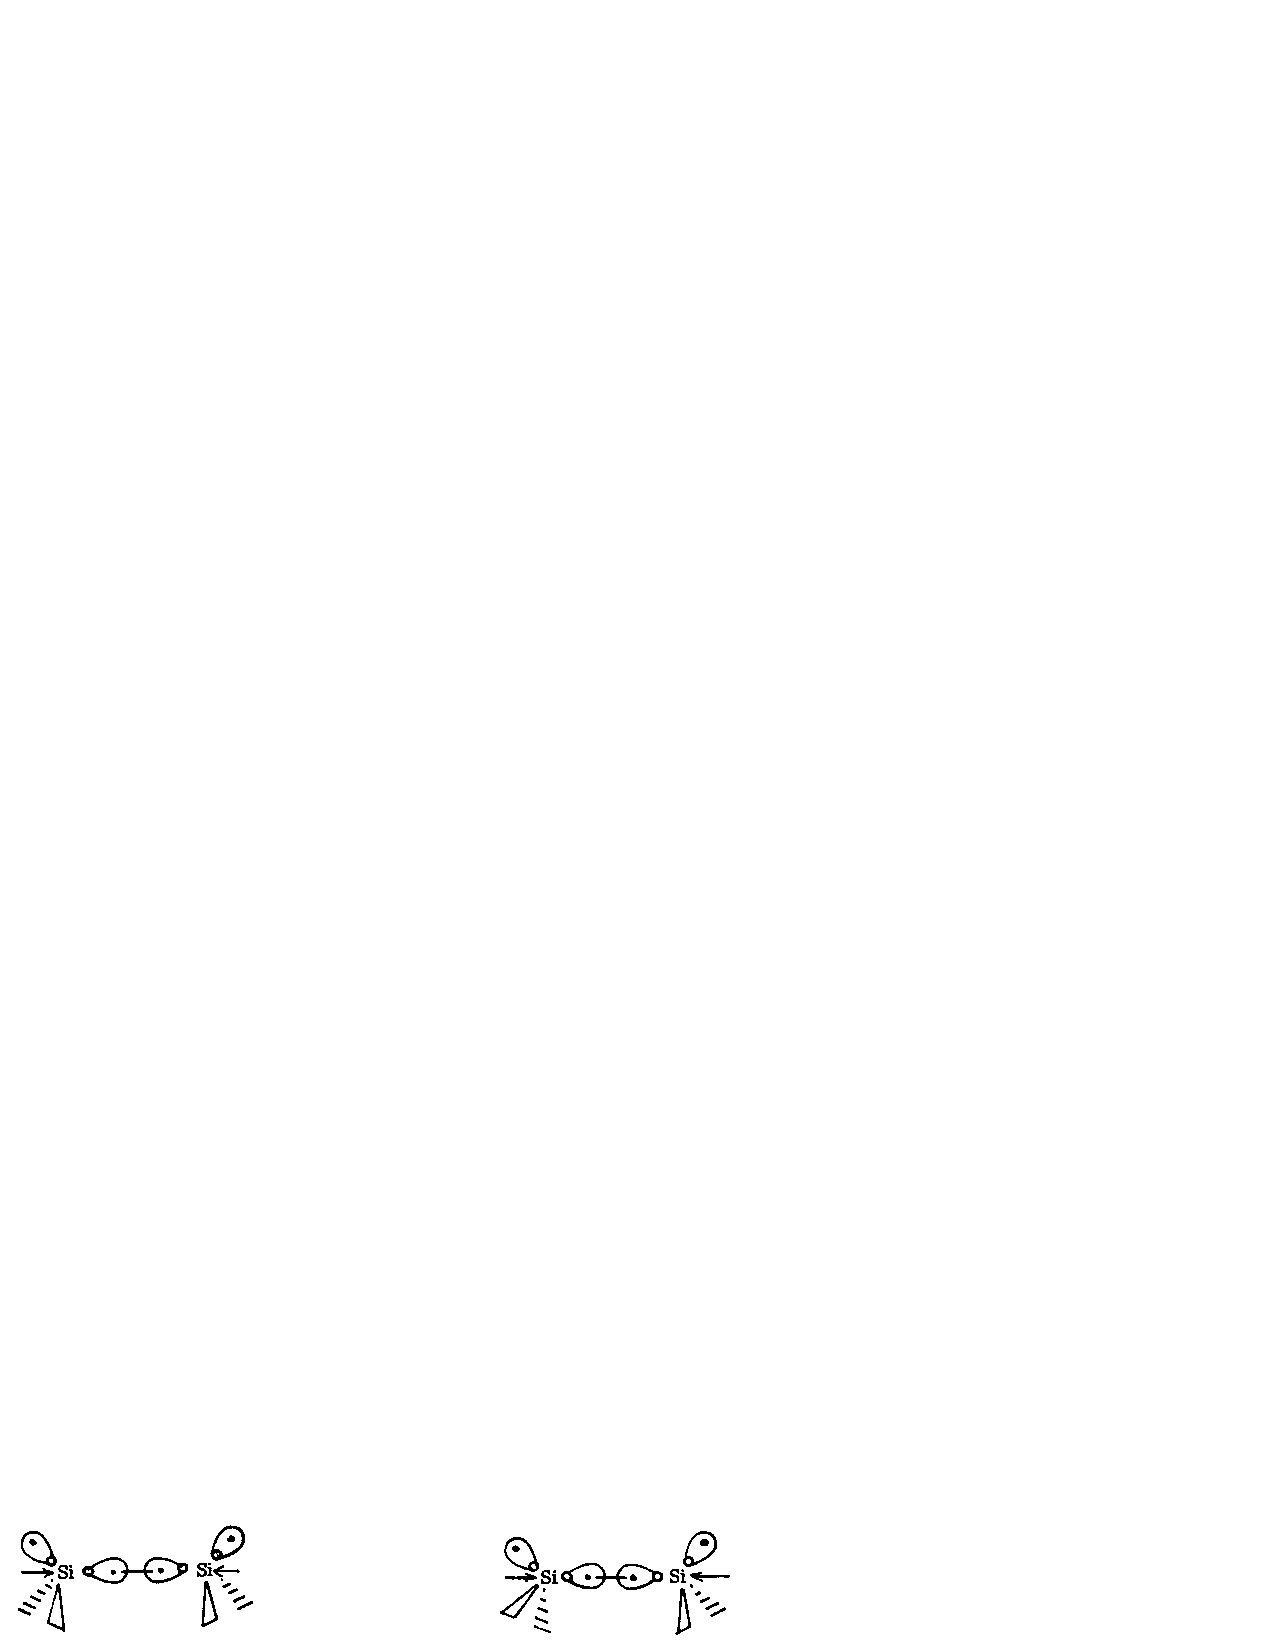
\includegraphics[scale=0.75]{fg8-20}
\end{center}
\caption{Surface Si atoms of (100) surface after reconstruction. The
actual orbitals are shown in Figure \ref{chap8-fig21}.}
\label{chap8-fig20}
\end{figure}

\begin{figure}
\begin{center}
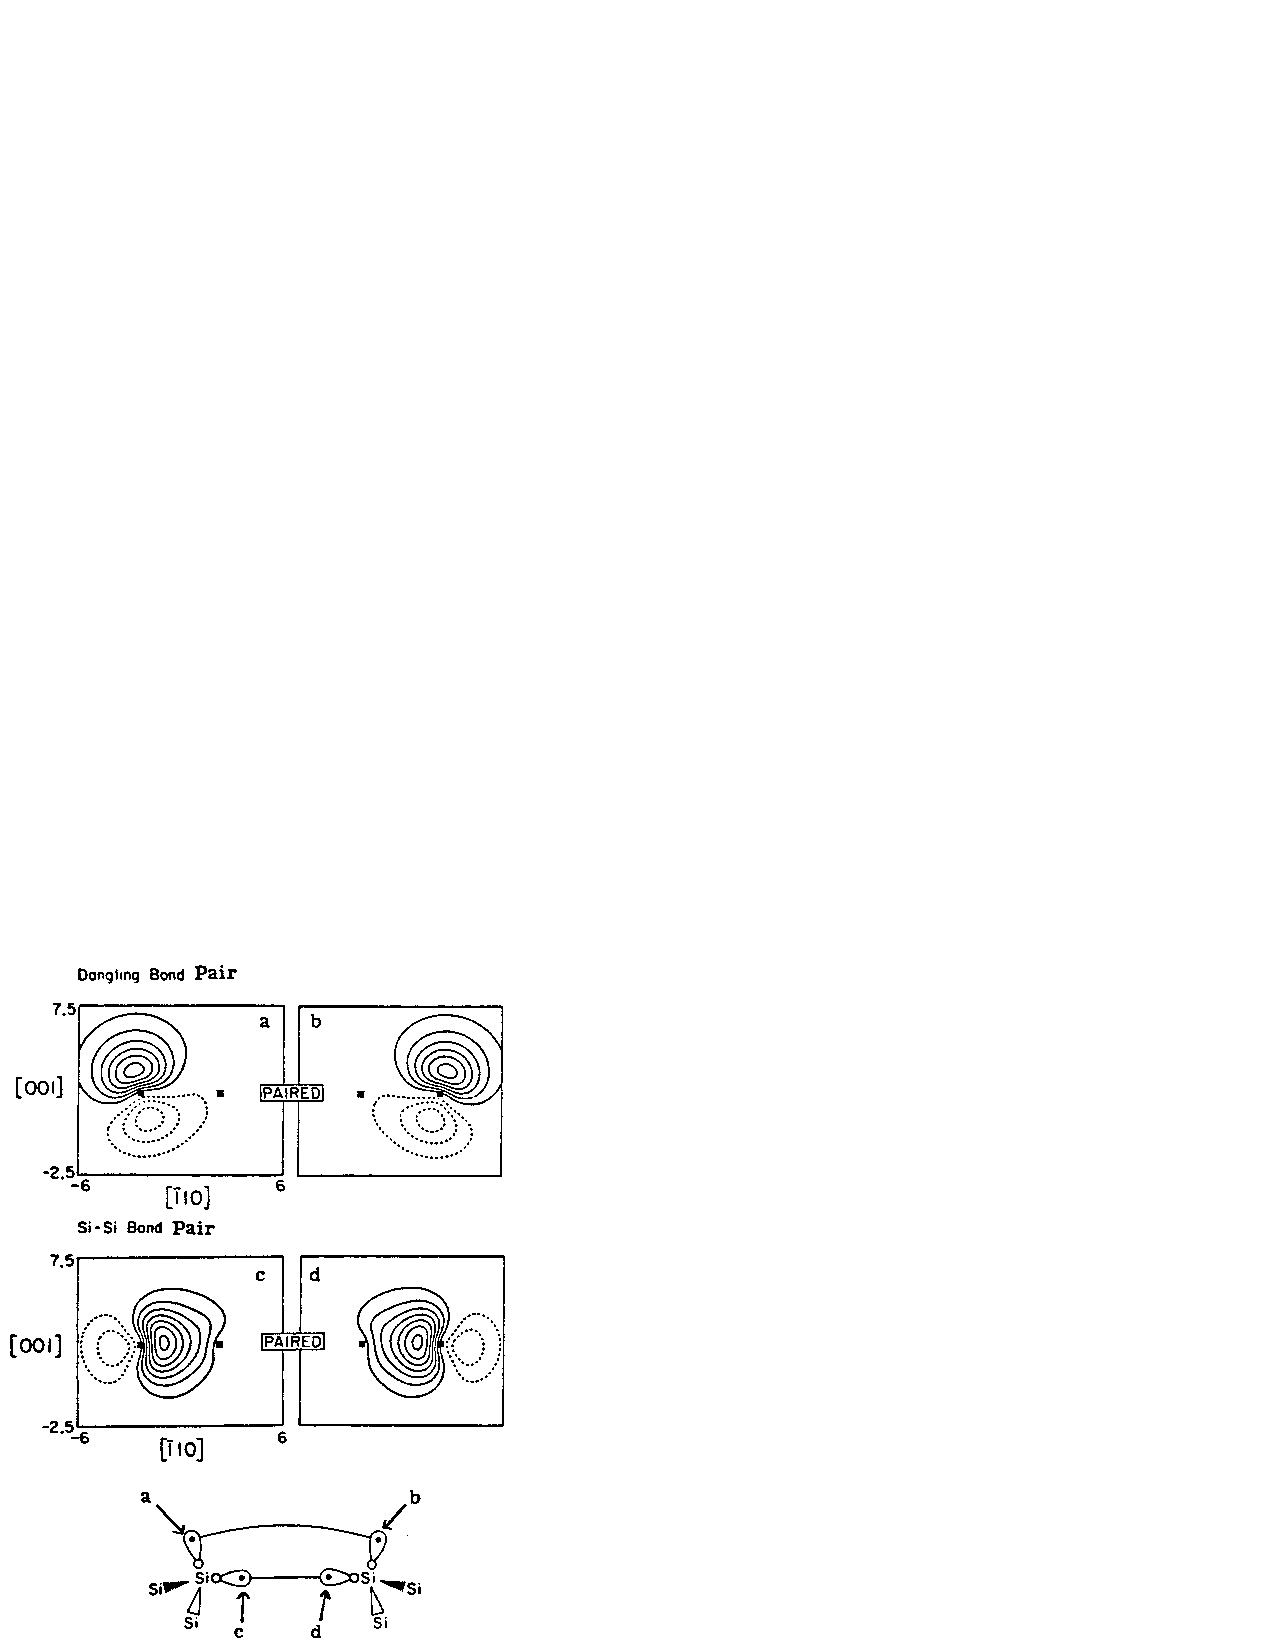
\includegraphics[scale=0.75]{fg8-21}
\end{center}
\caption{The GVB orbitals for one surface dimer of Si (100) surface,
singlet state: (a) the dangling bond pair, (b)the Si-Si bond pair
\cite{chap8-ref1}.}
\label{chap8-fig21}
\end{figure}

Thus, along the line of surface atoms corresponding to View B in
Figure \ref{chap8-fig18}, we expect the surface atoms to pair up or
dimerize as in Figure \ref{chap8-fig20}. This does not specify how the
pairing in one such row should be related to that in adjacent
rows. There are two simple possibilities, as indicated in Figure
\ref{chap8-fig22}.  First, the $P(2 \times 1)$ reconstruction of
Figure \ref{chap8-fig22}(a) and the $C(2 \times 2)$ reconstruction of
Figure \ref{chap8-fig22}(b).  Here the $P(2 \times 1)$ means that the
unit cell is twice as long as the $P(1 \times 1)$ cell in the x
direction, but the same length in the y direction.  The $C(2 \times
2)$ means that the unit cell is twice as big as the original $P(1
\times x 1)$ cell in both directions but that there are equivalent
atoms in both the corners and the center of the unit cell.

\begin{figure}
\begin{center}
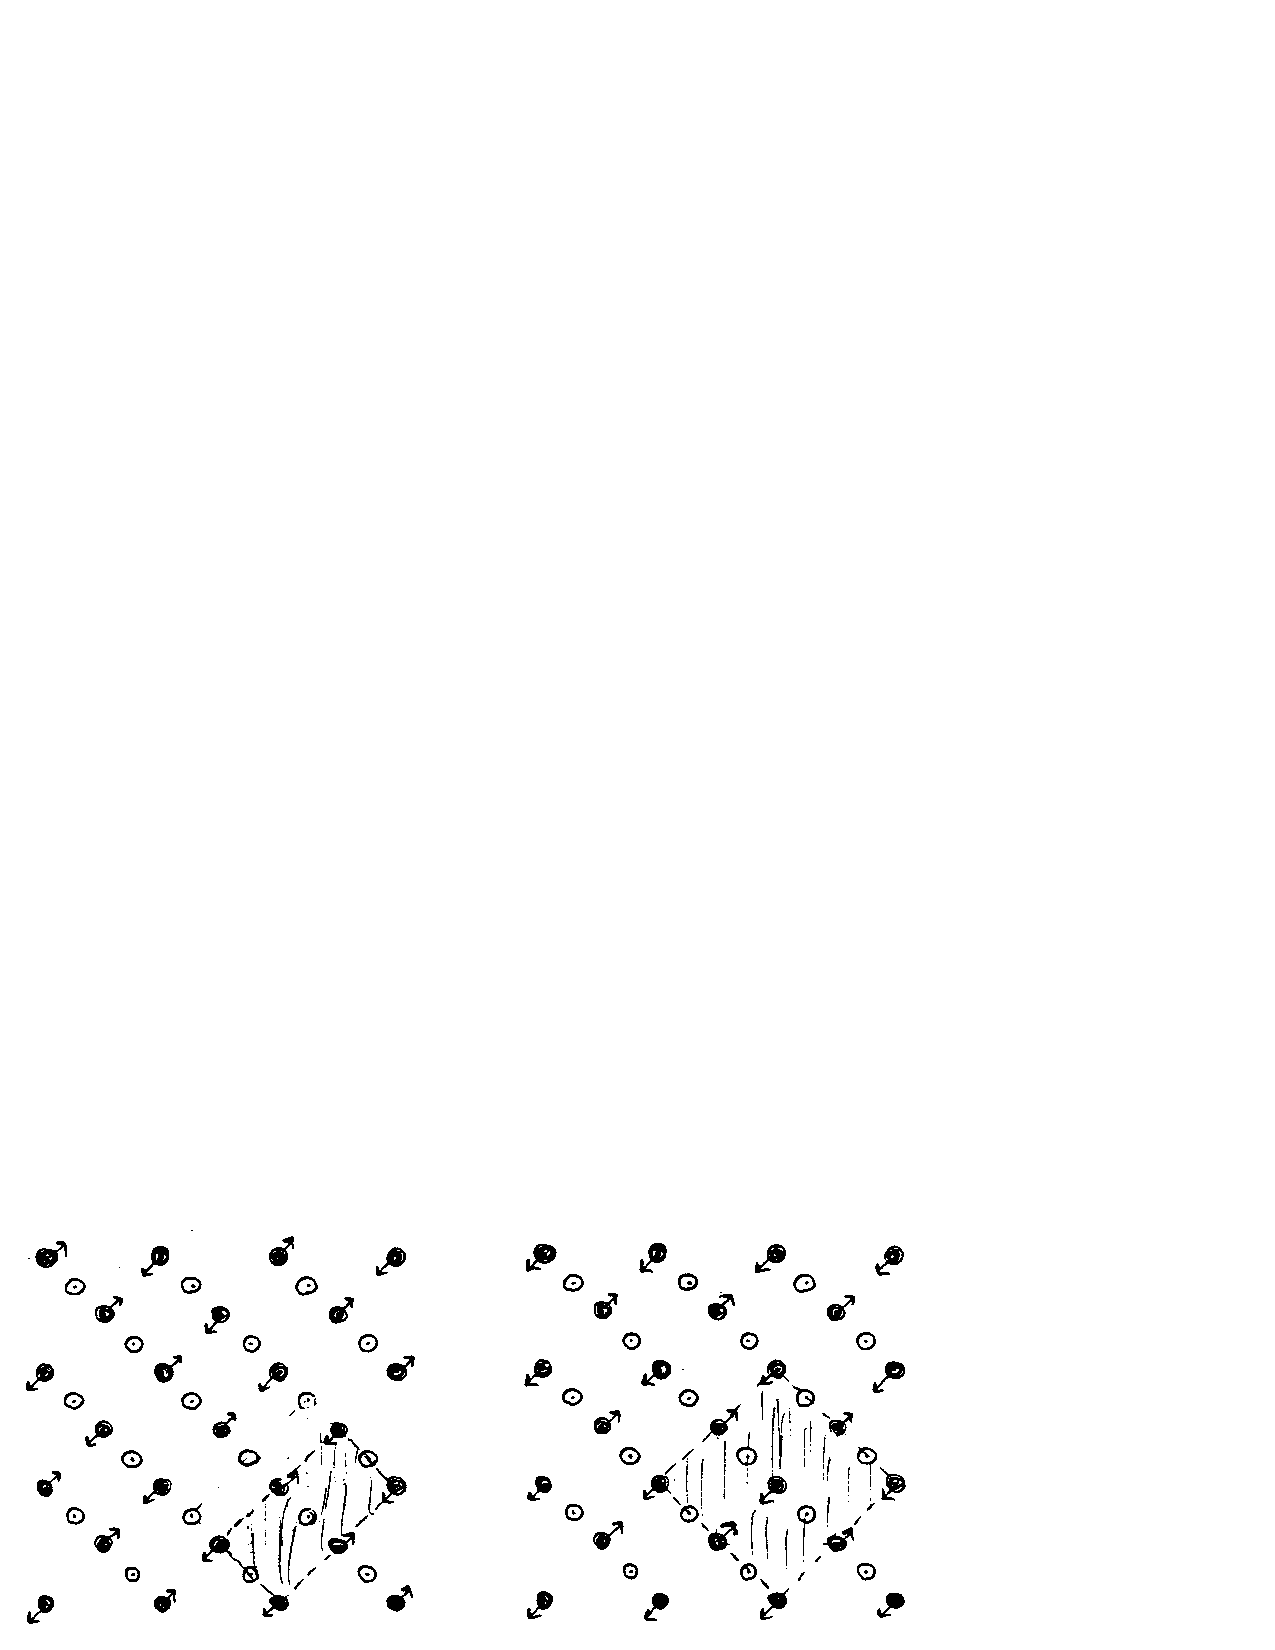
\includegraphics[scale=0.75]{fg8-22}
\end{center}
\caption{(a) $P(2 \times 1)$ reconstruction  of Si (100) surface. (b)
$C(2 \times 2)$ reconstruction of Si (100) surface.} 
\label{chap8-fig22}
\end{figure}

The theoretical calculations 
indicate that $C(2 \times 2)$ is not as favorable as $P(2 \times 1)$, 
due to the concerted motion of the subsurface atoms in the
latter case, and low energy electron diffraction, LEED, supports the 
$P(2 \times 1)$ structure.  He atom diffraction suggests that more 
complicated structures may also be 
present.

The (100) surface of Si is the technologically important one used in most 
semiconductor applications, it leads to growth of a very good oxide layer, 
i.e., no electron traps.

\subsubsection{Si(110) Surface}

A second interesting surface of Si is obtained by cutting the cubic
unit cell of Figure \ref{chap8-fig6} along one diagonal, leading to
Figure \ref{chap8-fig23}, called the (110) surface.  In Figure
\ref{chap8-fig23}, the outline of the original cubic unit cell is
shown by dashed lines.  Here we see that each surface atom is bonded
to two other surface atoms plus one below the surface.  Thus, there is
one nonbonding electron left in a dangling bond orbital hybridized
away at an angle to the surface, as indicated in Figure
\ref{chap8-fig24}.

\begin{figure}
\begin{center}
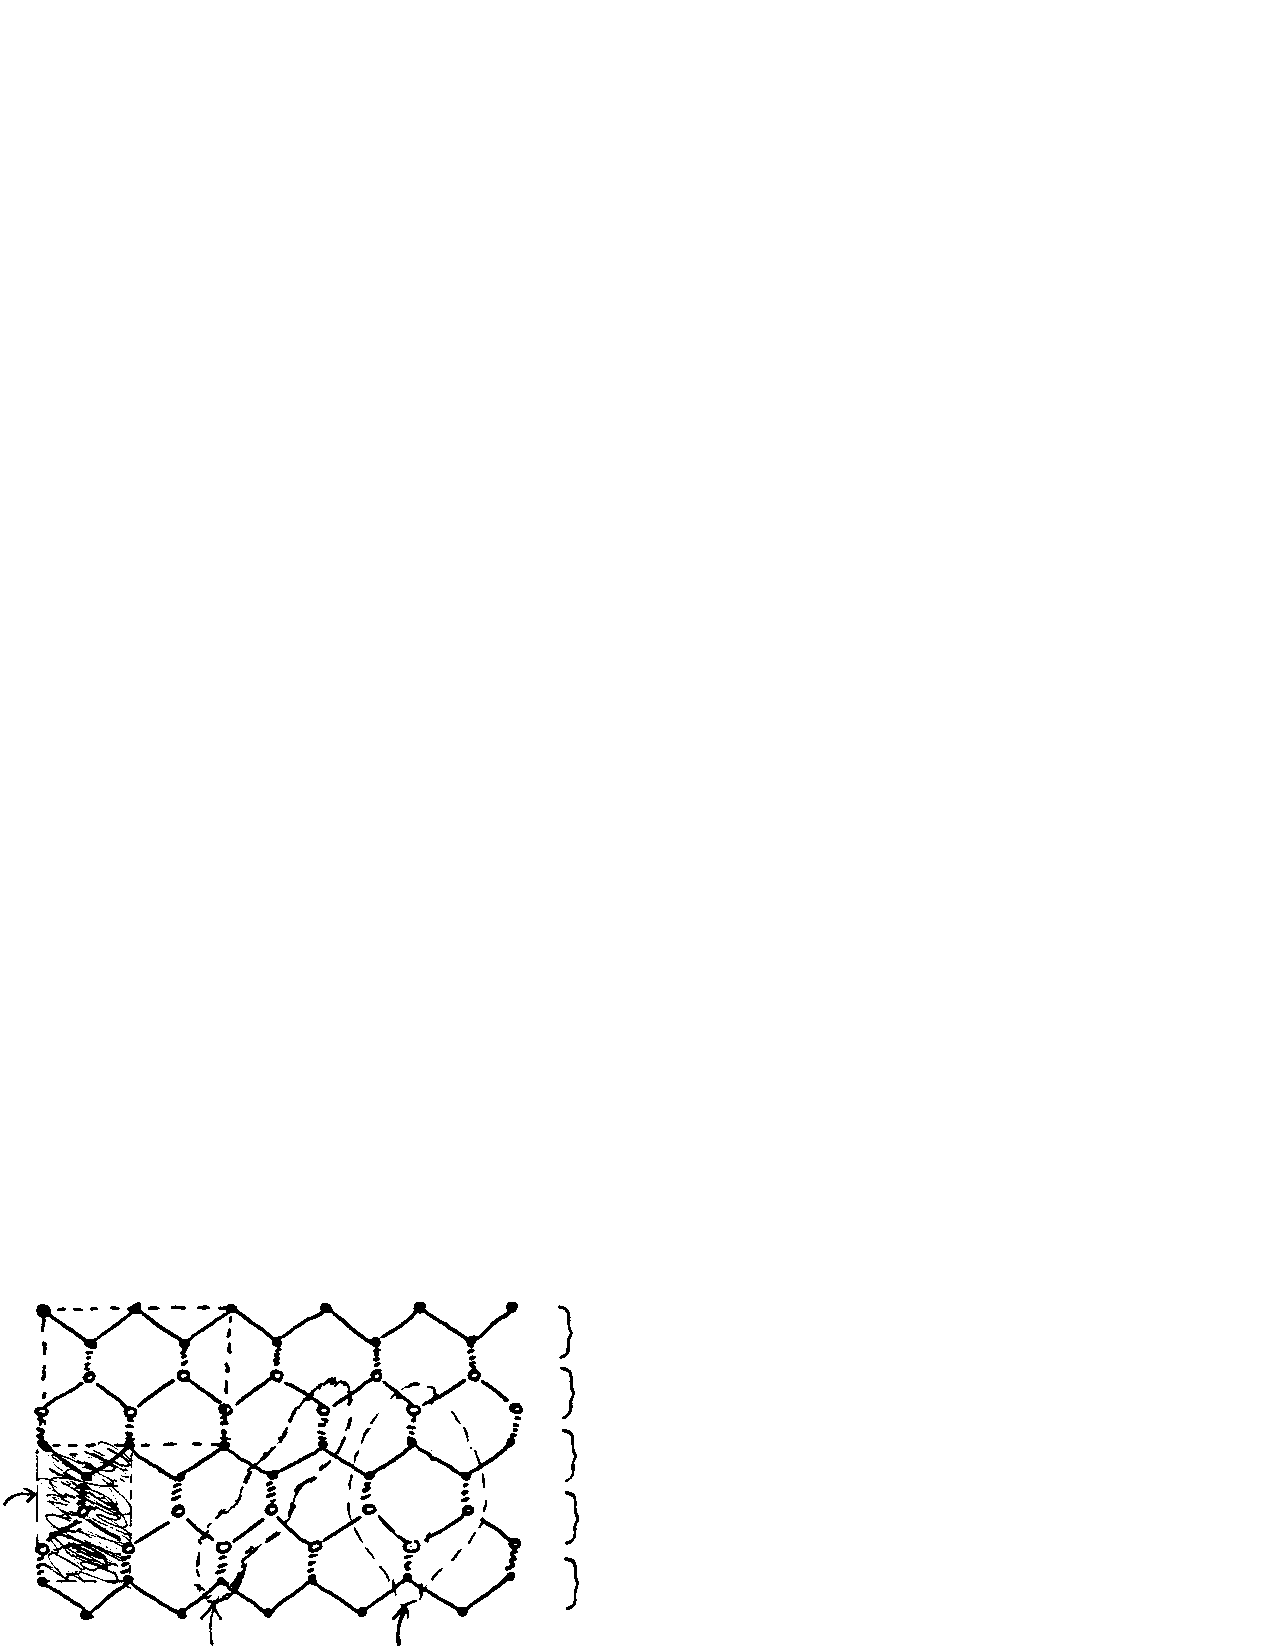
\includegraphics[scale=0.75]{fg8-23}
\end{center}
\caption{The Si (110) surface. The outline of the original cubic unit
cell is shown by dashed lines.}
\label{chap8-fig23}
\end{figure}

\begin{figure}
\begin{center}
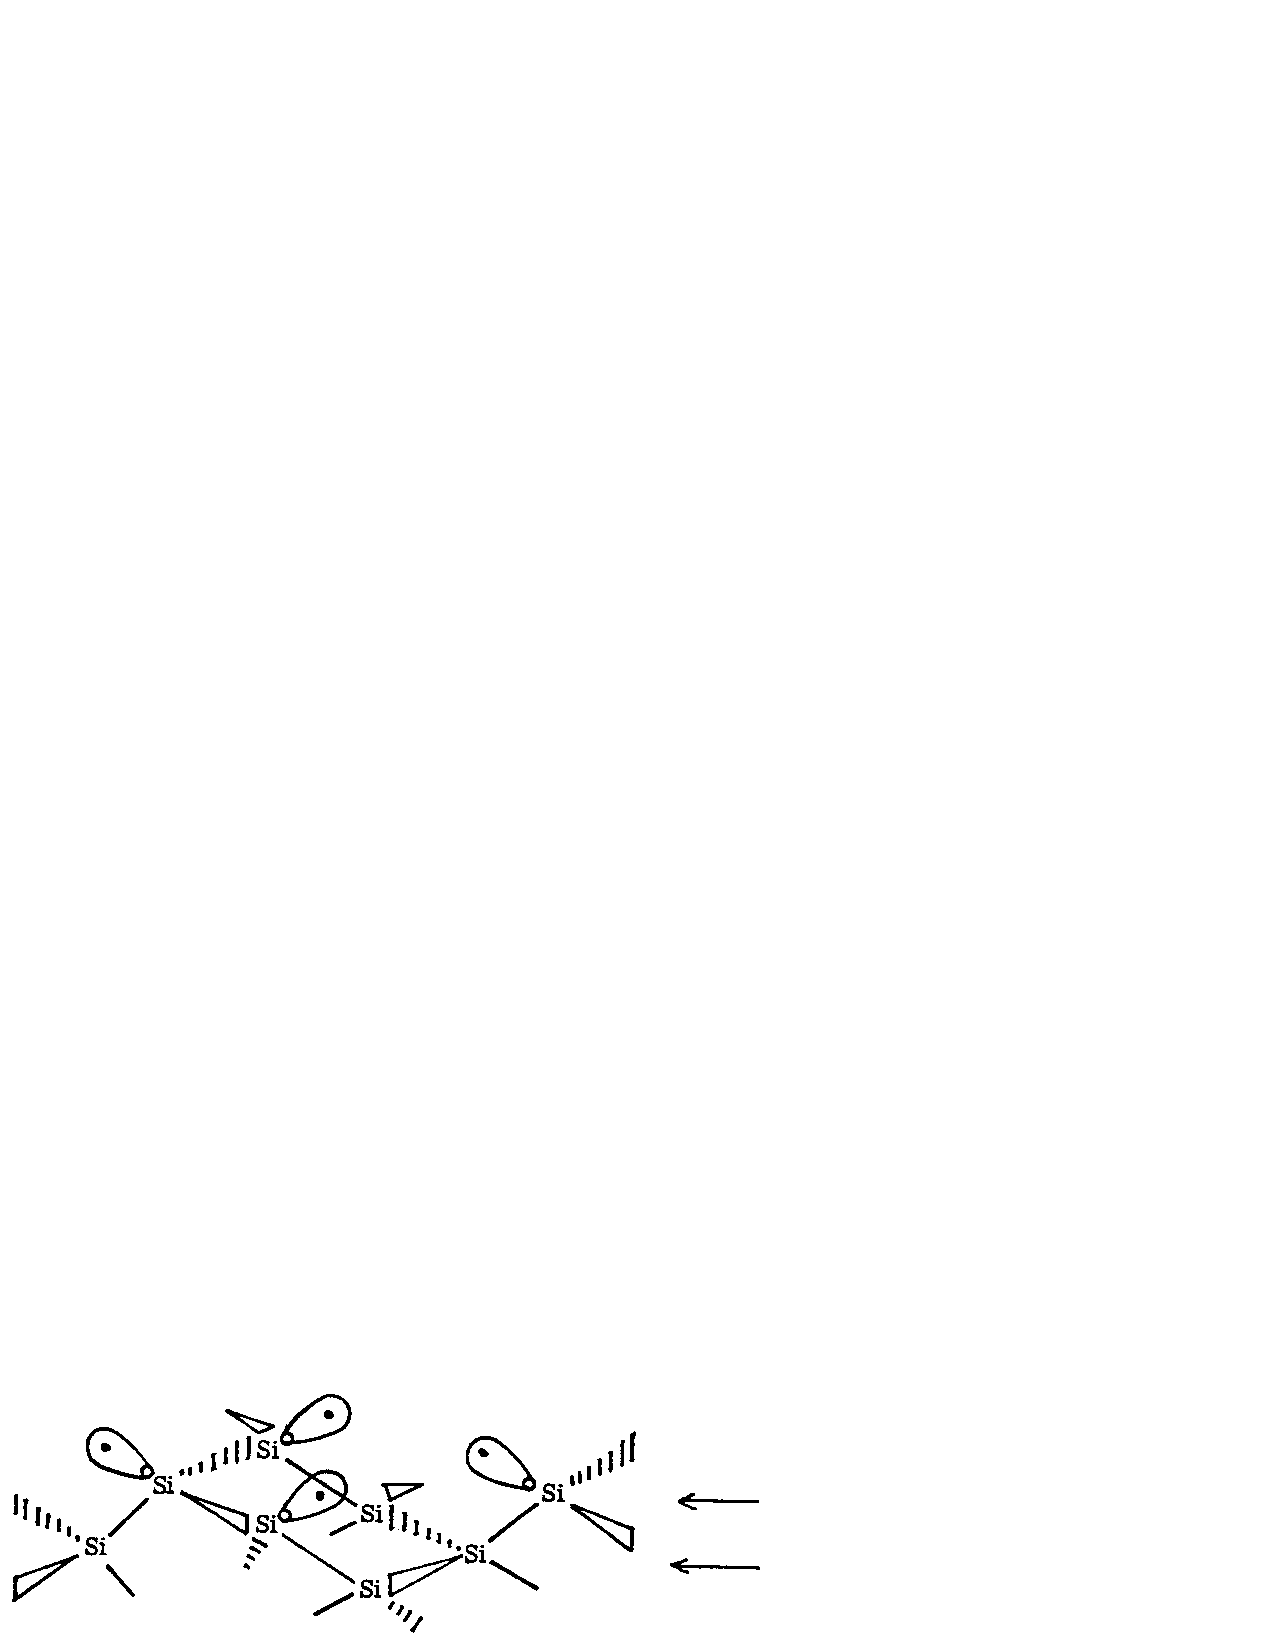
\includegraphics[scale=0.75]{fg8-24}
\end{center}
\caption{}
\label{chap8-fig24}
\end{figure}

As one proceeds along the sequence of atoms in Figure
\ref{chap8-fig25}, one sees a sequence of dangling bond orbitals.

\begin{figure}
\begin{center}
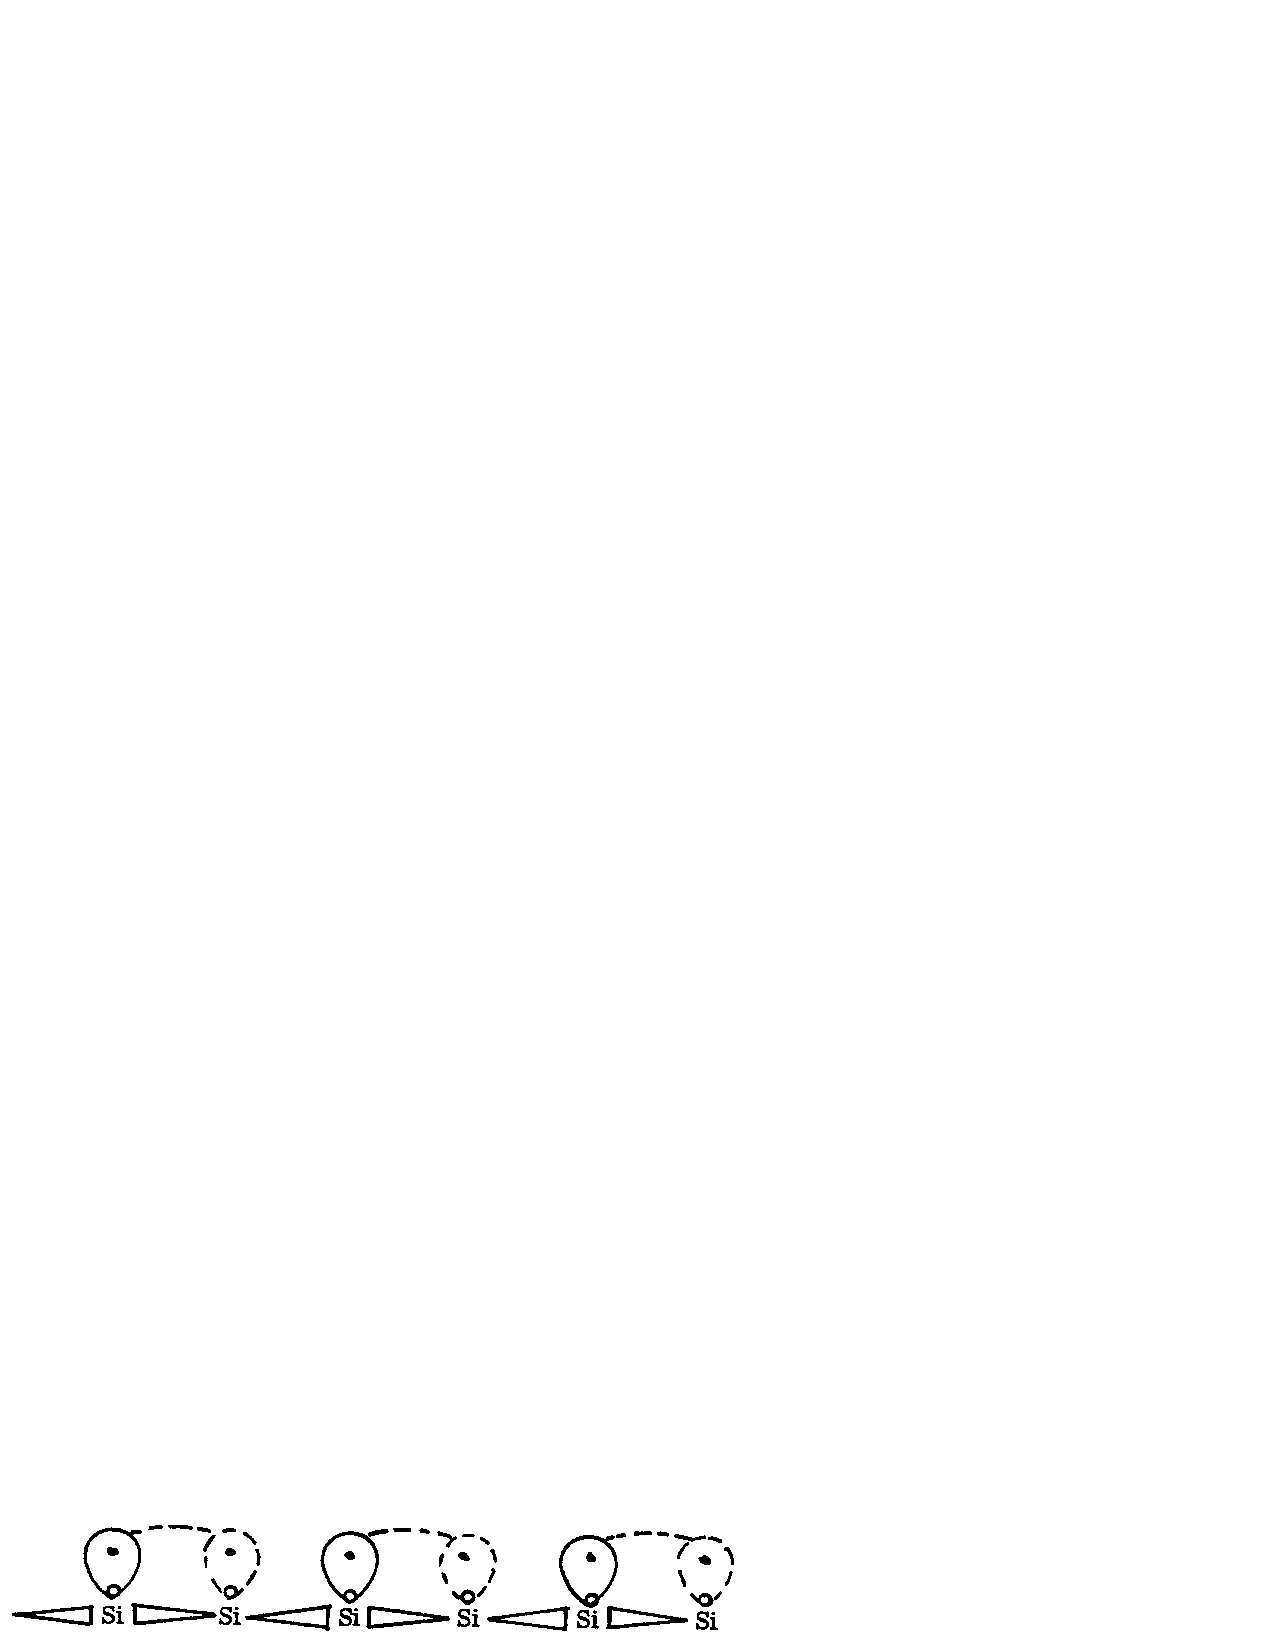
\includegraphics[scale=0.75]{fg8-25}
\end{center}
\caption{Side view of the Si (110) structure.}
\label{chap8-fig25}
\end{figure}

The atoms of such a state would be expected to reconstruct so as to
get an alternating sequence of pi bonds, as indicated in Figure
\ref{chap8-fig25}.  This would lead to a $P(2 \times 1)$ surface
structure corresponding to the dashed outline in Figure \ref{chap8-fig25}.

\subsubsection{Si (111) Surface}

The third interesting surface of Si is sketched in Figure
\ref{chap8-fig26}.  Here the $P(1 \times 1)$ unit cell is shaded.
This is obtained by cutting Figure \ref{chap8-fig2} perpendicular to a
body diagonal.

\begin{figure}
\begin{center}
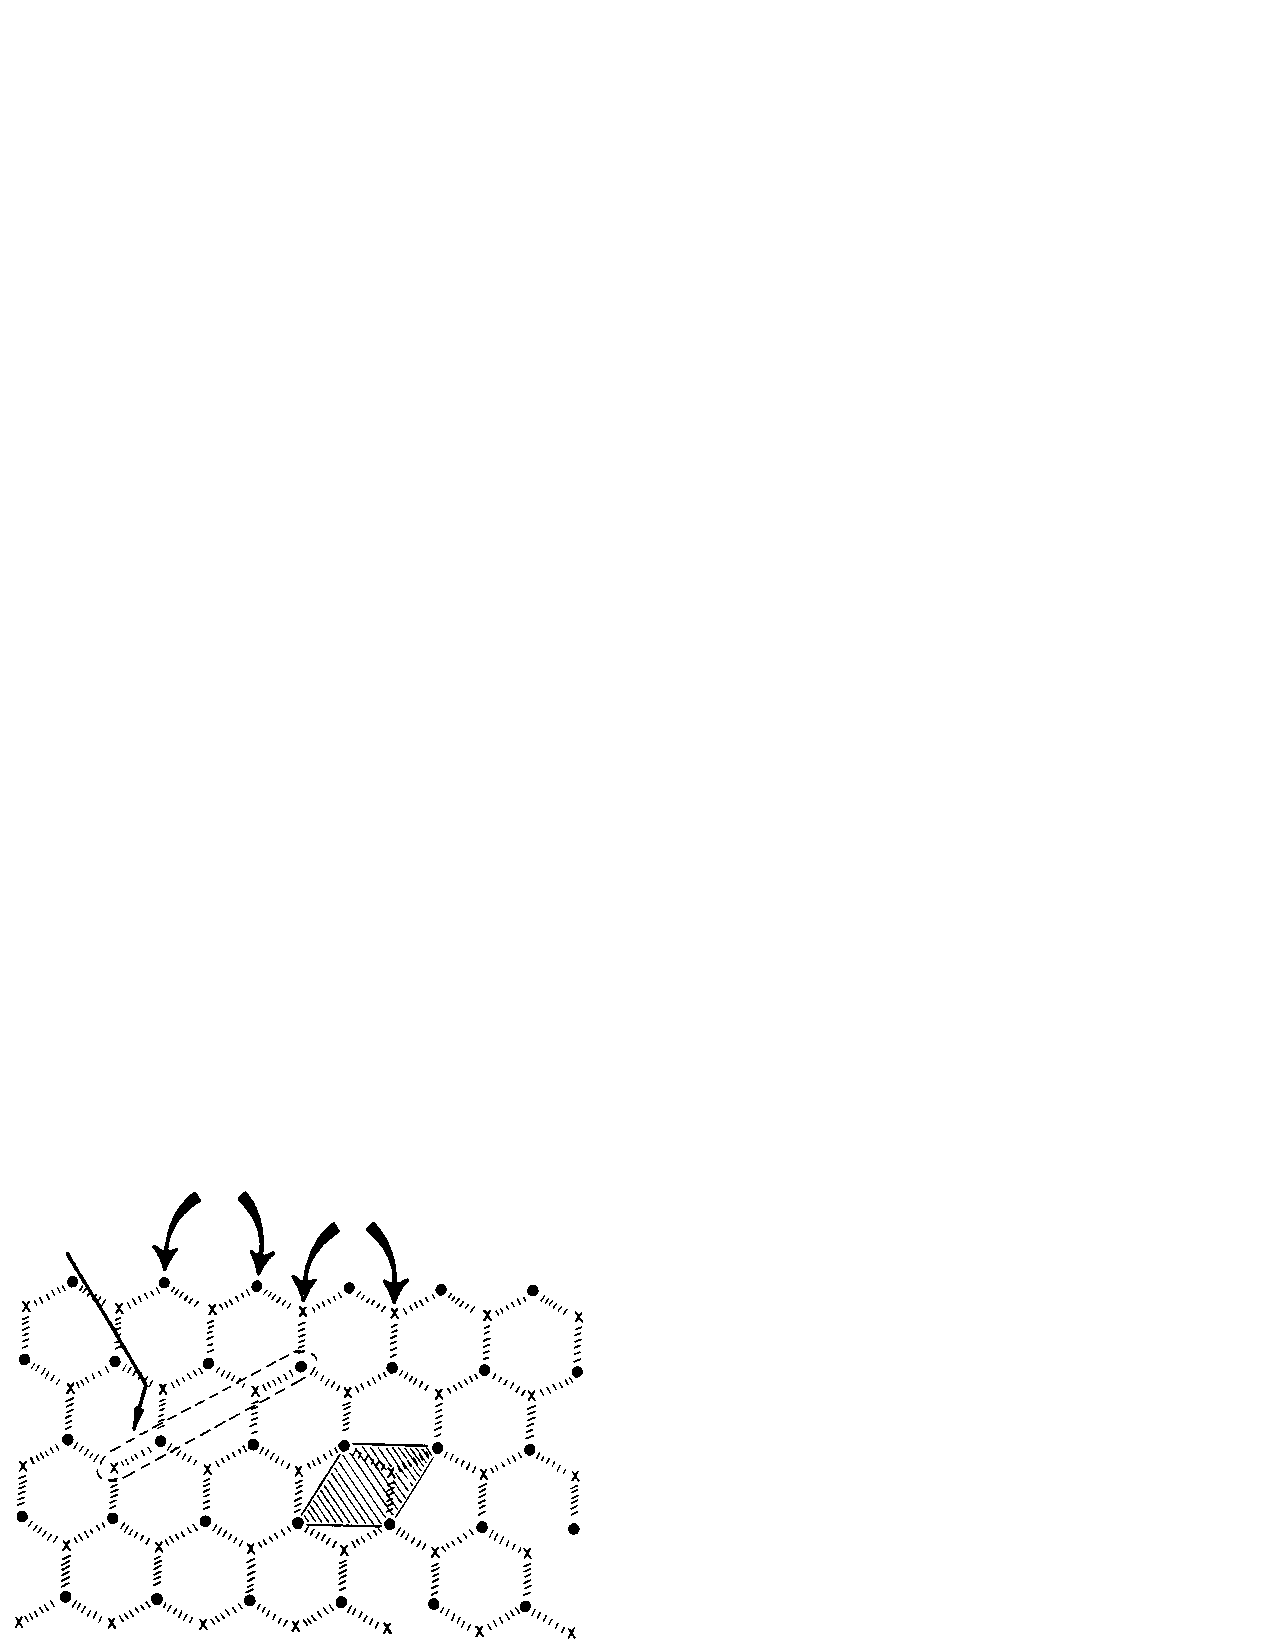
\includegraphics[scale=0.75]{fg8-26}
\end{center}
\caption{The Si (111) surface. The $P(2\times 1)$ unit cell is shaded.}
\label{chap8-fig26}
\end{figure}

Here each surface atom is bonded to three subsurface atoms, as
indicated in the cross section given in Figure \ref{chap8-fig27},
corresponding to View A in Figure \ref{chap8-fig26}.

\begin{figure}
\begin{center}
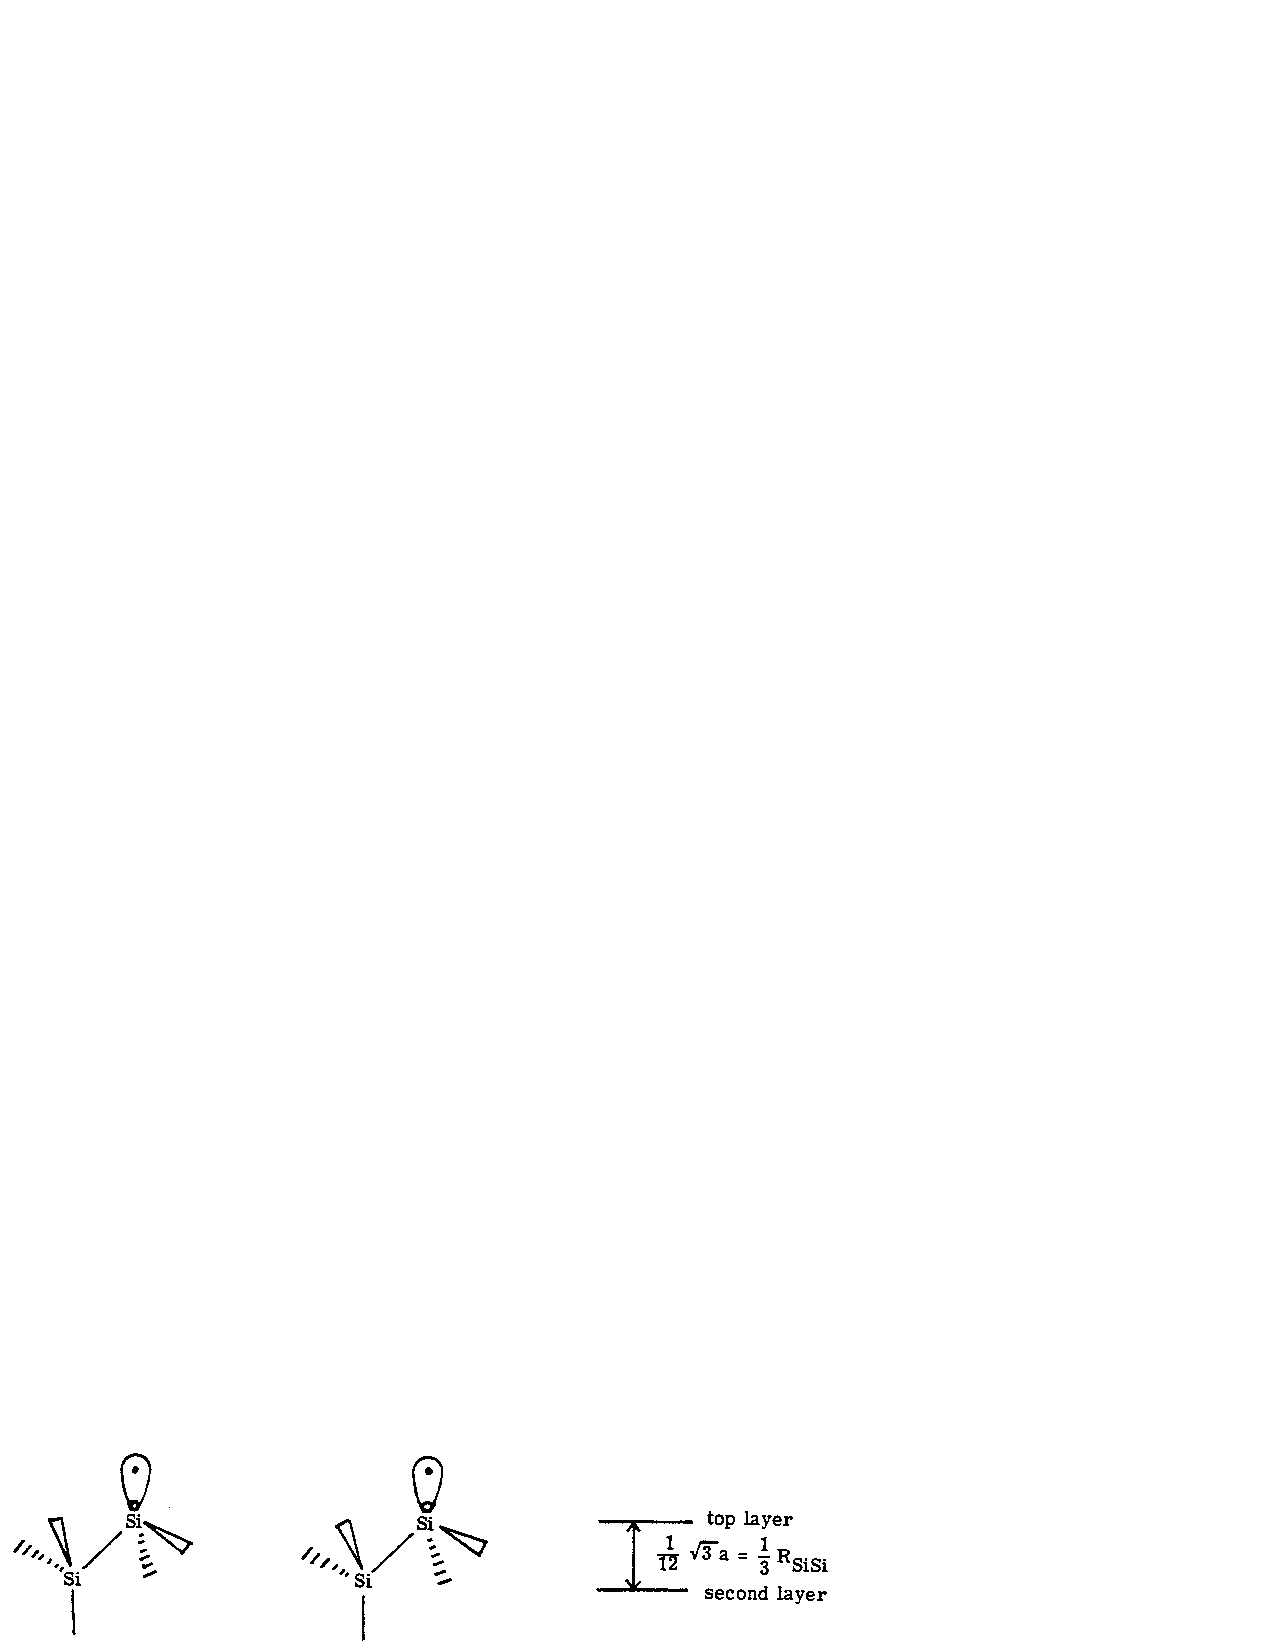
\includegraphics[scale=0.75]{fg8-27}
\end{center}
\caption{}
\label{chap8-fig27}
\end{figure}

The (111) surface is obtained by cleaving the crystal of Si.  Thus, this is 
probably the lowest energy surface.  An estimate of the surface energy is 
given in the next section.

Each surface Si in Figure \ref{chap8-fig26} is bonded symmetrically to
three subsurface Si atoms and hence there is not much freedom of
movement.  Indeed, both theory and experiment indicate that the
surface Si relaxes by 0.14 \AA\ away from the vacuum.  This is 18
\% of the original distance between the top two layers, ${1 \over
3} R_{SiSi} = 0.78$\AA.  Only a small relaxation is expected since
SiH$_3$ adopts a pyramidal geometry with `angle' HSiH 110$^{\circ}$.
The fact that this angle is larger than tetrahedral, 109.5$^{\circ}$,
suggests that the surface Si would move away from vacuum, as observed.

For the (111) surface of diamond, much larger distortions would be
expected since CH$_3$ prefers to be planar.  Of course, this desired
planar geometry could also be achieved by moving the second layer C
toward the vacuum. Indeed, if the first two layers of Figure
\ref{chap8-fig26} are moved toward each other to be in the same plane,
the result is the hexagonal plane of graphite in which each C can make
pi bonds to the adjacent atoms. This peeling off of the top two layers
to form graphite would leave behind the original third layer, which
would now appear just as in Figures \ref{chap8-fig26} and
\ref{chap8-fig27}.  This in turn could peel off a second layer of
graphite. There is evidence that this effect does occur and that
stabilization of the (111) cleavage surface of diamond requires
binding of H to the dangling bond orbitals of the surface atoms, as
indicated in Figure \ref{chap8-fig28}.

\begin{figure}
\begin{center}
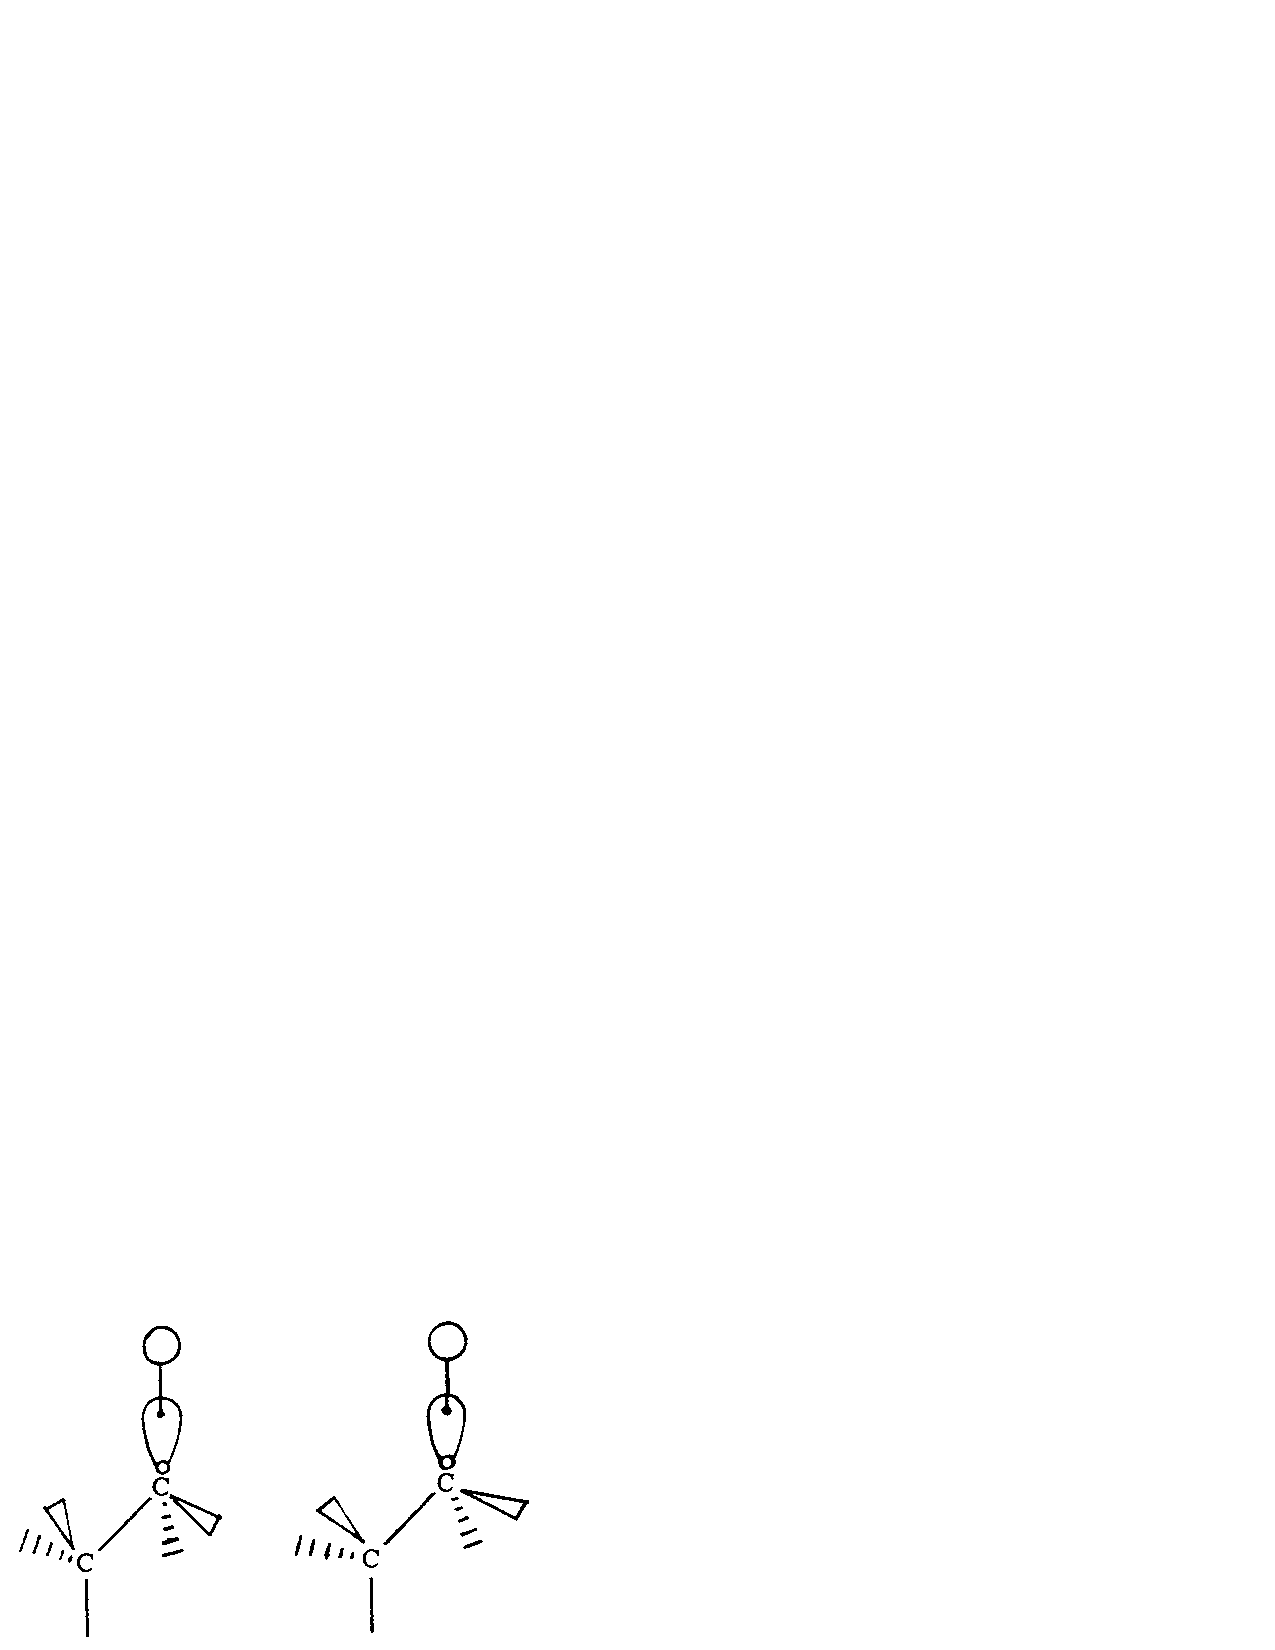
\includegraphics[scale=0.75]{fg8-28}
\end{center}
\caption{Stabilization of diamond (111) surface using H atoms.}
\label{chap8-fig28}
\end{figure}

Thus, our description of Si(111) has an infinite array of singly-occupied 
dangling bond orbitals at the surface well separated, 3.8 \AA. from each other. 
Experimentally it is known that freshly cleaved Si leads to a $P(2 
\times 1)$ structure, if $T < 350^{\circ}$C; however, numerous
experimental attempts have failed to establish the structure for this
reconstructed surface.  Theorists have filled the void and there are
currently two popular models, as indicated in Figures
\ref{chap8-fig29} and \ref{chap8-fig30}.


\begin{figure}
\begin{center}
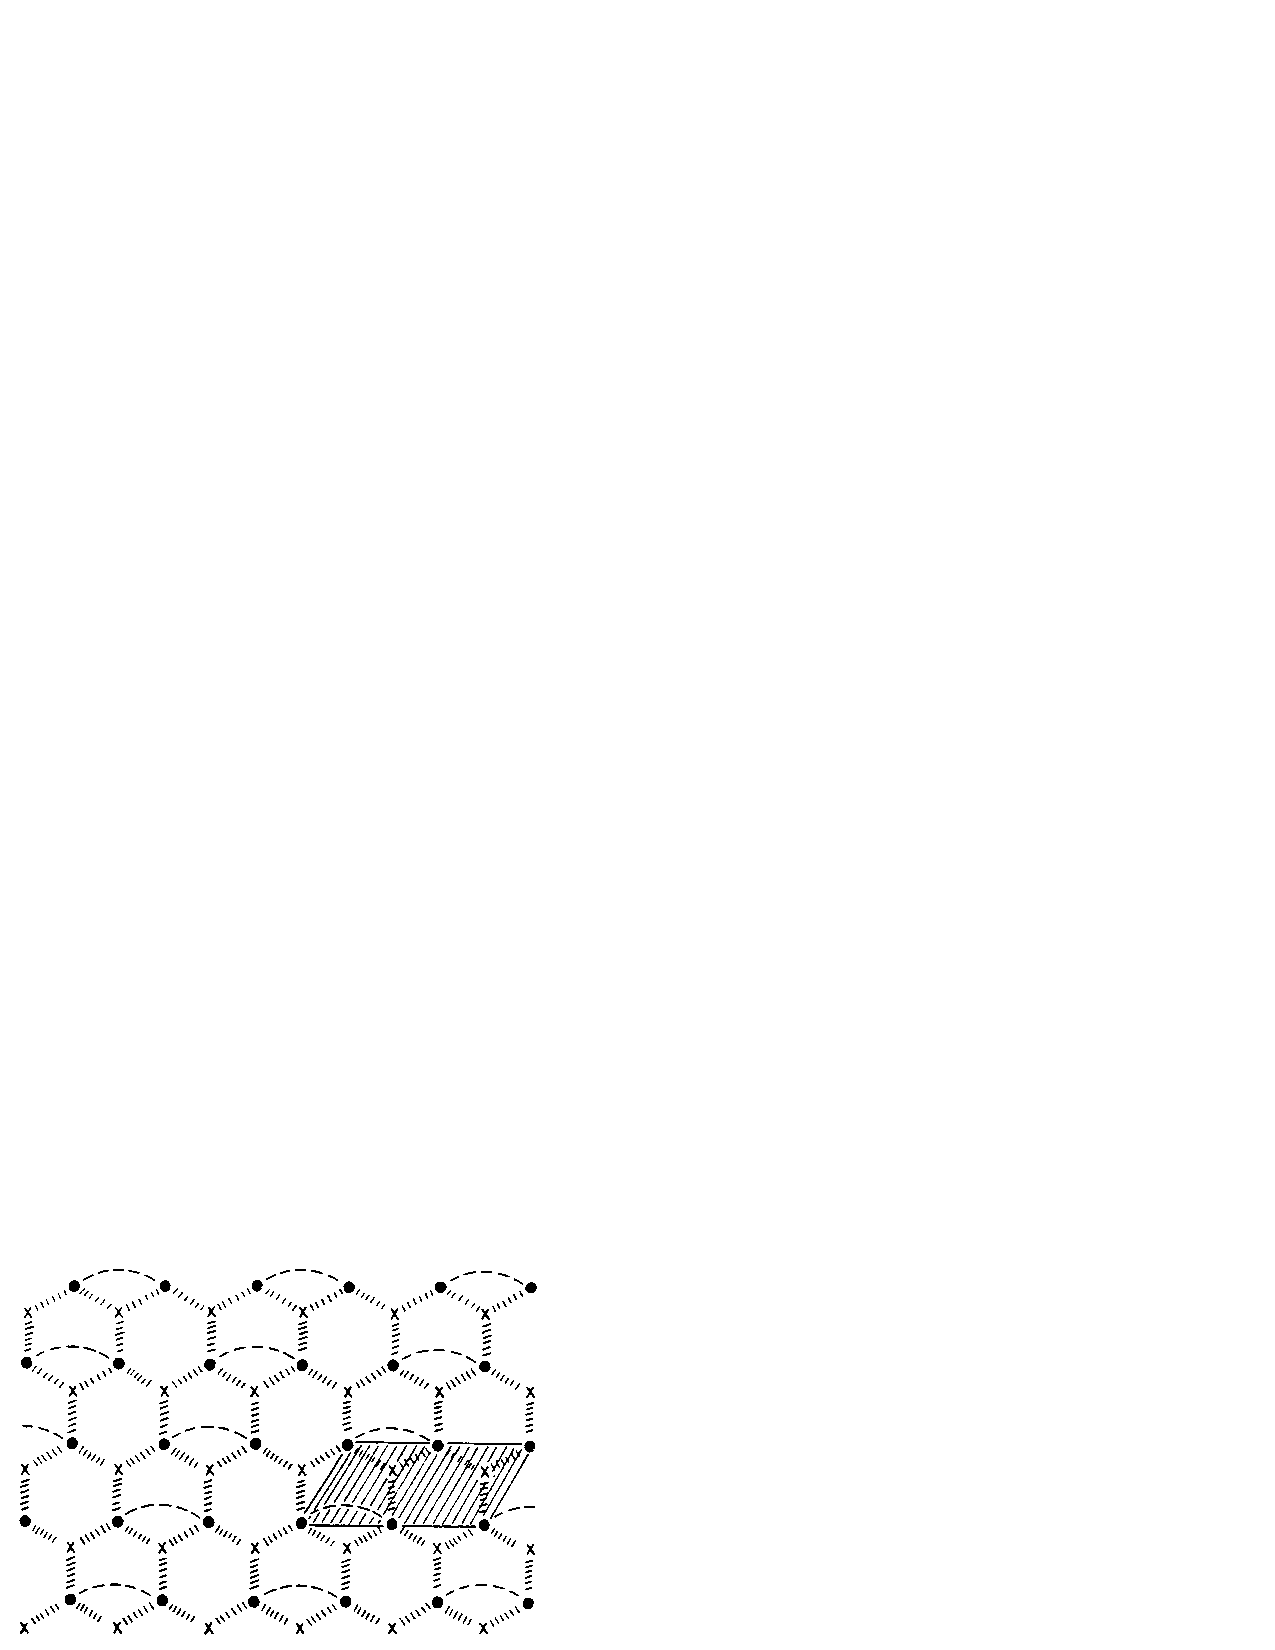
\includegraphics[scale=0.75]{fg8-29}
\end{center}
\caption{The valence bond pairing model of the $P(2 \times 1)$
reconstruction of Si(111).  The unit cell is shaded.} 
\label{chap8-fig29}
\end{figure}

In Figure \ref{chap8-fig29}, we assume that although the dangling bond
orbitals interact but weakly, they are ${2 \over 3} \sqrt{6} R_{SiSi}
= 1.633 R_{SiSi} = 3.84$\AA\ apart, there is some stabilization
resulting from spin pairing of adjacent pairs.  This pairing would
lead to slight distortion and, hence, to a lower symmetry, as
indicated in Figure \ref{chap8-fig29}, this is referred to as the VB model.

Another model that has been suggested is the pi-bonded model in Figure 
\ref{chap8-fig30}.  Here we add in a new layer of atoms in zig-zag
chains that bond to the old surface atoms.

\begin{figure}
\begin{center}
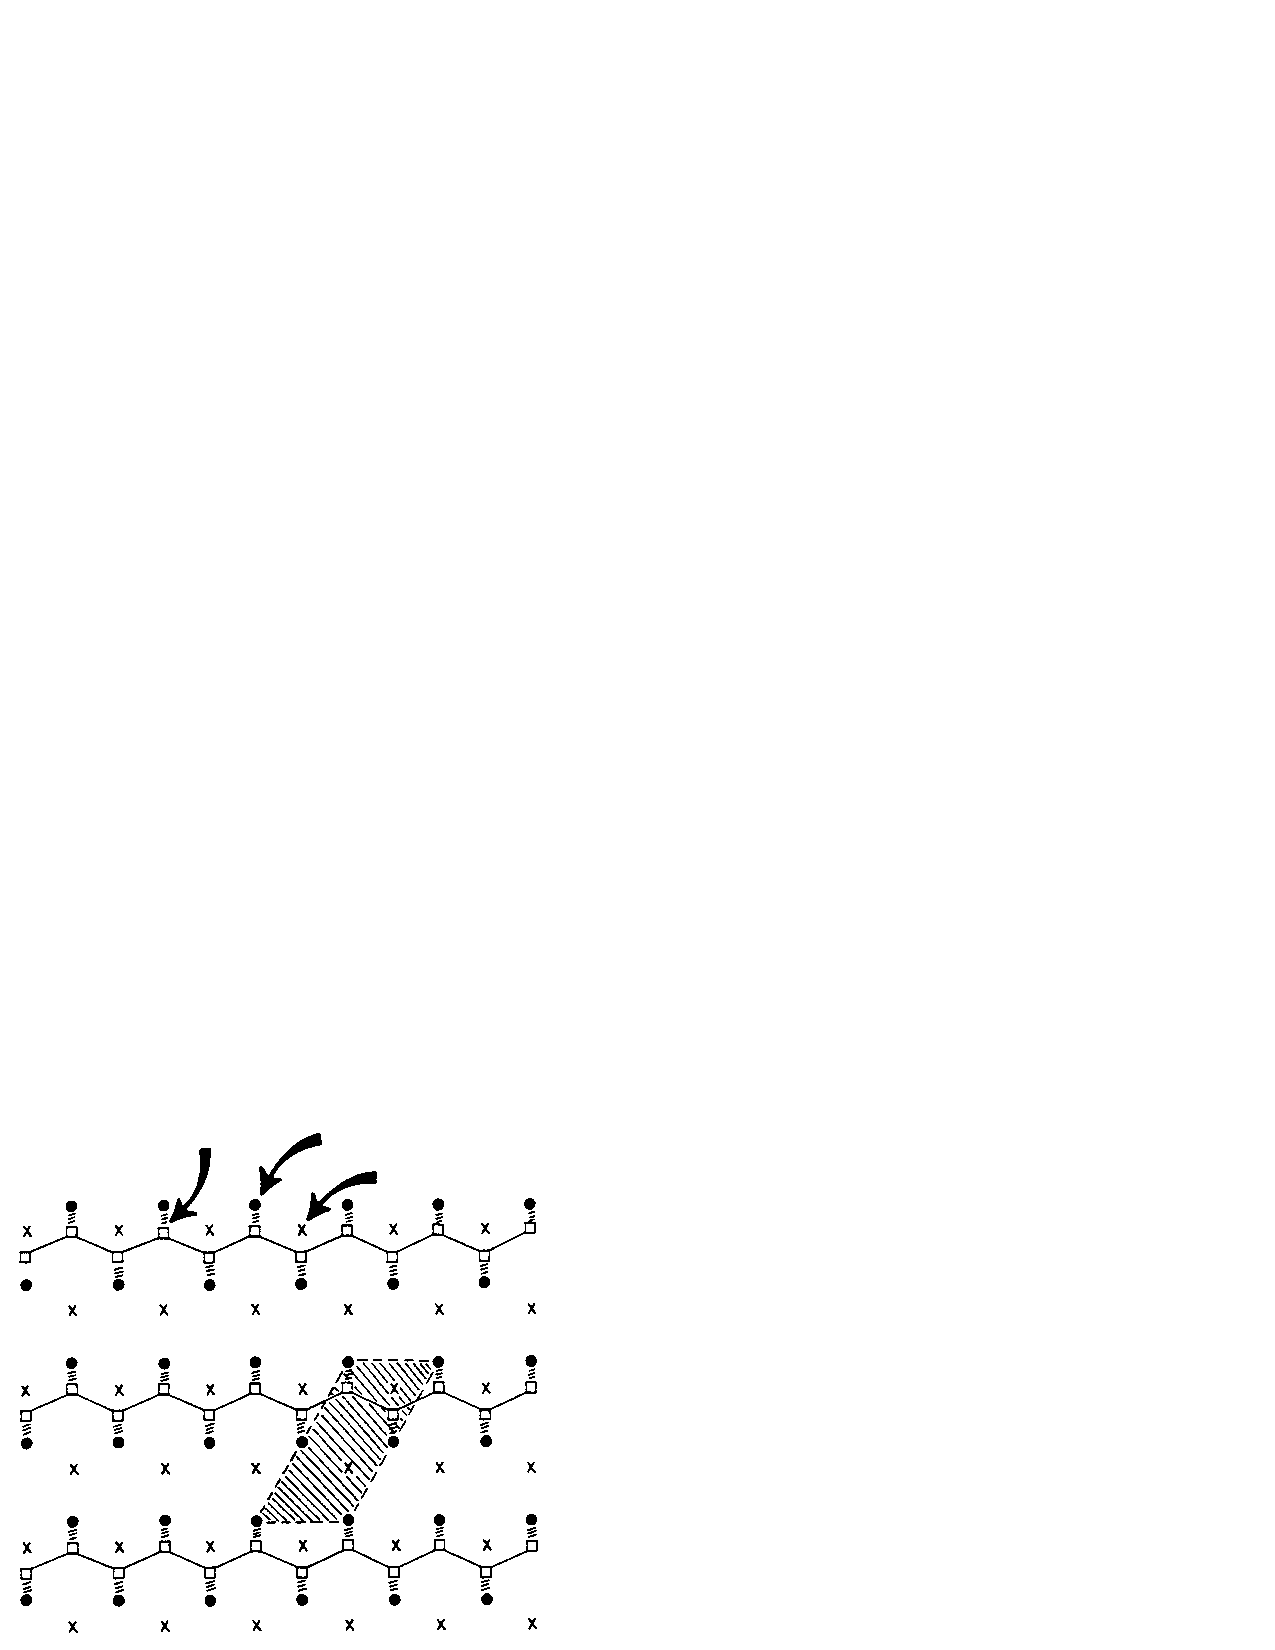
\includegraphics[scale=0.75]{fg8-30}
\end{center}
\caption{The $\pi$-bonded model of the $P(2 \times 1)$ 
reconstruction of Si (111).  The unit cell is shaded.  }
\label{chap8-fig30}
\end{figure}

Both the VB and $\pi$-bonded models explain current experimental data,
but most physicists are tending toward the $\pi$-bonded model.

Most confusing about the Si(111) surface is that heating to 
500$^{\circ}$K leads to the irreversible conversion to a structure 
that has a $7 \times 7$ unit cell.  Thus, there may be 49 
inequivalent surface Si atoms in the unit cell of the stable surface! 
Despite numerous experimental and theoretical
studies over the last 20 years, there is no convincing structural 
information about this surface.  At
1170$^{\circ}$K, there is a reversible transformation to a $(1 \times 
1)$ structure, and one can retain this $(1 \times 1)$
structure by rapid quenching.  In these cases, it is not known for sure 
whether the surface really has the $(1 \times 1)$ structure or whether 
it is completely disordered, with the structure being that of
the sublayer.

\subsubsection{The Surface Energy}

The problem is to stimate which of the surfaces should be most stable for Si, 
(100), (110), and/or (111).  The answer is, first,
determine how many bonds must be broken per unit area, and then 
consider how important is each of the various types of broken bonds.
The surface areas will be related back to the cubic lattice 
parameter $\alpha$.

\begin{enumerate}
\item Si (100) surface.  In the dashed region, area = 
$\alpha^2$, of Figure \ref{chap8-fig18}(a), there are two surface Si
atoms, each representing two broken bonds. Therefore,
\begin{equation}
N_{(100)} = 2 \times {2 \over \alpha^2} = {4 \over \alpha^2}
\end{equation}

\item Si (110) surface.  In the dashed region, area = 
$\sqrt{2}\alpha^2$, of Figure \ref{chap8-fig23}, there are four
surface atoms, each representing one broken bond. Therefore,
\begin{equation}
N_{(100)} = {4 \over \sqrt{2}\alpha^2} = {2 \sqrt{2} \over 
\alpha^2} = {2.82 \over \alpha^2}.
\end{equation}

\item Si (111) surface.  For the (111) surface, a fast way 
to obtain the surface area is to note that for a diamond structure the
second nearest neighbors are ${\alpha \over \sqrt{2}}$ apart, see
Figure \ref{chap8-fig2}, so that the area of the unit cell in Figure
\ref{chap8-fig26} is
\begin{equation}
{\alpha \over \sqrt{2}} \left[ {\sqrt{2} \over 2} {\alpha \over 
\sqrt{2}} \right] = {1 \over 4} \sqrt{3} \alpha^2 .
\end{equation}
There is one bond broken in this area so that
\begin{equation}
N_{111} = {4 \over \sqrt{3}\alpha^2} = {2.31 \over \alpha^2}
\end{equation} 
Thus, ignoring any differences in bond energies and neglecting 
reconstruction, we expect that the (111) surface is most stable.
\end{enumerate}


\begin{figure}
\begin{center}
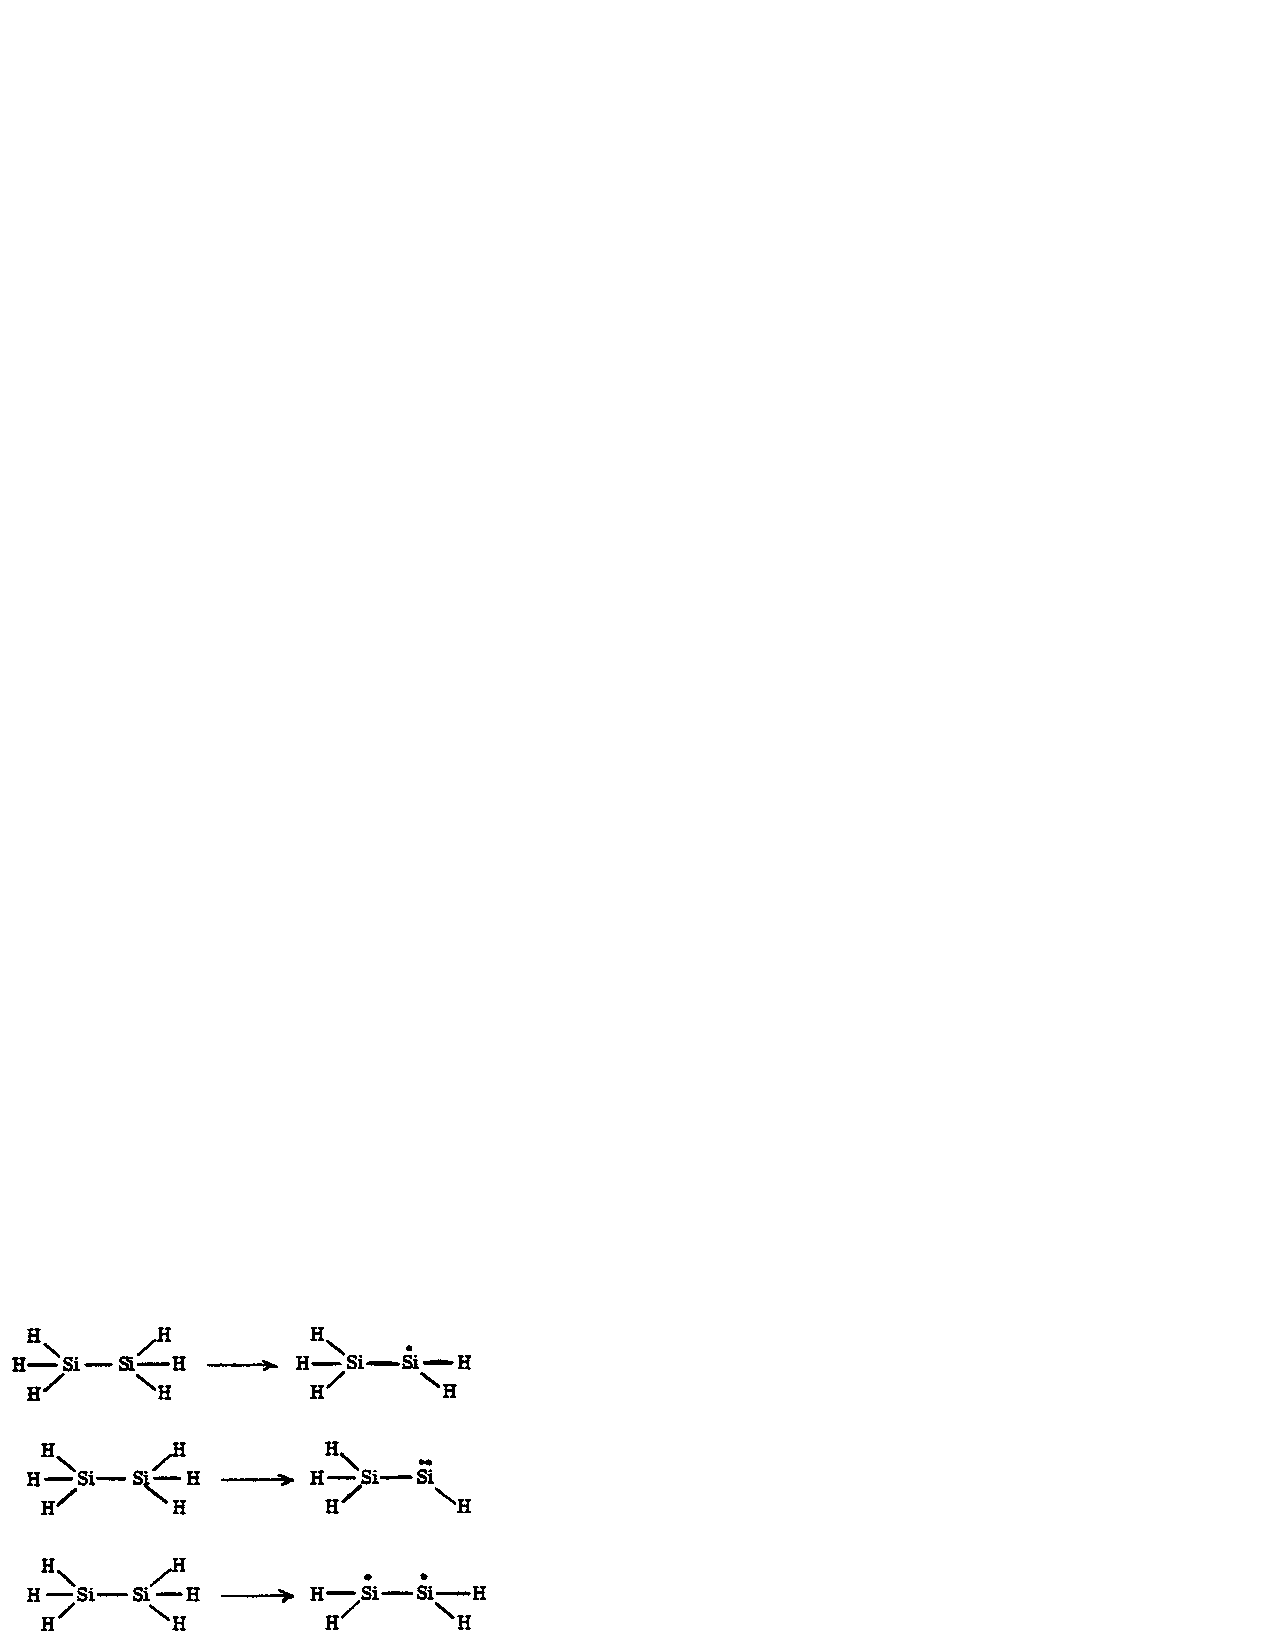
\includegraphics[scale=0.75]{fg8-31}
\end{center}
\caption{(a) $\Delta H = 86$ kcal (74); (b)$\Delta H = 160$ kcal
(136); (c) $\Delta H = 154$ kcal (130).}
\label{chap8-fig31}
\end{figure}

In order to get some handle on the differences in bonding, consider
the thermochernistry for Si systems shown in Figure \ref{chap8-fig31}.
Although these bond energies refer to Si-H rather than Si-Si bonds,
the relative magnitudes may apply to the Si-Si case. Since
\begin{equation} 
H_3 Si - Si H_3 \rightarrow H_3 Si + Si H_3 ~~~ \Delta H = 74 {\rm 
kcal}
\end{equation} 
we will use the reduced energies in parentheses, leading to
\begin{eqnarray}
\Delta H_{111} &=& {2.31 \over \alpha^2} \times 74 = {171 \over 
\alpha^2} {\rm kcal}\cr
\Delta H_{110} &=& {2.82 \over \alpha^2} \times {130 \over 2} = {183 
\over \alpha^2}\cr
\Delta H_{100} &=& {4 \over \alpha^2} {136 \over 2} = {272 \over 
\alpha^2}.
\end{eqnarray}
Thus, the (111) surface is again expected to be most stable.

Next we must consider reconstruction. The biggest change is for (100) where 
a new Si-Si bond is formed.  However, calculations indicate that this energy 
stabilization is less than 20 kcal. Thus, our conclusion is that for 
Si the (111) surface is most stable.


